% ============================================================

\documentclass[sensors,article,submit,pdftex,moreauthors]{Definitions/mdpi}


%=================================================================
% MDPI Sensors-style layout controls for journal submission
% - one-column MDPI article format
% - table captions above tables
% - figure captions below figures
% - compact full-width tables with tabularx
% - centered figures with controlled widths
%=================================================================
\setlength{\tabcolsep}{4pt}
\renewcommand{\arraystretch}{1.12}
\newcommand{\mdpitablefont}{\footnotesize}
\newcommand{\figfull}{\textwidth}
\newcommand{\figwide}{0.92\textwidth}
\newcommand{\figmedium}{0.78\textwidth}
\newcommand{\figsmall}{0.68\textwidth}
\usepackage{multirow}
% Define AIstatement command
\newcommand{\AIstatement}[1]{\section*{AI Statement}#1}

% Fix fancyhdr headheight warning
\setlength{\headheight}{20.0pt}
\addtolength{\topmargin}{-8.0pt}

\firstpage{1}
\makeatletter
\setcounter{page}{\@firstpage}
\makeatother
\pubvolume{1}
\issuenum{1}
\articlenumber{0}
\pubyear{2026}
\copyrightyear{2026}
\datereceived{ }
\daterevised{ }
\dateaccepted{ }
\datepublished{ }

%=================================================================
\Title{Beyond Data Leakage: An Explainable Predictive Maintenance Benchmarking Framework with Generative Augmentation and Human-Centred Reporting for Industry~5.0}

\newcommand{\orcidauthorA}{}

\Author{
Mohammed S. AlKahtani$^{1}$,
Tayyab Rehman$^{2}$,
Abdullah Almasad$^{3}$,
Qazi Salman Khalid$^{4}$,
Muzzamil Mustafa$^{5}$
}

\AuthorNames{Mohammed S. AlKahtani, Tayyab Rehman, Abdullah Almasad, Qazi Salman Khalid, Muzzamil Mustafa}

\address{
$^{1}$ Department of Industrial Engineering, College of Engineering,
King Saud University, P.O.\ Box 800, Riyadh 11421, Saudi Arabia;
moalkahtani@ksu.edu.sa (M.S.A.)\\
$^{2}$ Department of Information Engineering, Computer Science, and Mathematics,
University of L'Aquila, 67100 L'Aquila, Italy;
tayyab.rehman@graduate.univaq.it (T.R.)\\
$^{3}$ Department of Industrial Engineering, College of Engineering,
King Saud University, P.O.\ Box 800, Riyadh 11421, Saudi Arabia;
aalmasad@ksu.edu.sa (A.A.)\\
$^{4}$ Department of Industrial Engineering,
University of Engineering \& Technology, Peshawar 25000, KPK, Pakistan;
qazisalman@uetpeshawar.edu.pk (Q.S.K.) \\
$^{5}$ Department of Information Engineering, Computer Science, and Mathematics,
University of L'Aquila, 67100 L'Aquila, Italy;
muzzamil.mustafa@graduate.univaq.it (M.M.)\\

}

\corres{Correspondence: tayyab.rehman@graduate.univaq.it}


%=================================================================
\abstract{Predictive maintenance~(PdM) in Industry~5.0 demands
classifiers that are accurate, explainable, and free from evaluation
artefacts. Most AI4I~2020 studies retain five target-derived
failure-indicator columns during training, a data-leakage flaw that
inflates F1 by up to 13~points.
We present \textit{XAI-PdMNet-Bench}, a leakage-safe benchmarking
framework combining process-informed feature construction,
imbalance-aware held-out evaluation, CTGAN augmentation validated by
Kolmogorov--Smirnov and correlation-matrix fidelity tests, SHAP
attribution, and template-based operator reporting
($n{=}9{,}973$; 3.31\,\% failure rate).
All failure-indicator columns are removed and a 25-feature
representation is evaluated on a shared imbalanced test set
($n{=}1{,}993$; 66~failures, 1{,}927~normal). XGBoost achieves
precision~=~1.000, recall~=~0.742, F1~=~0.852, ROC-AUC~=~0.989,
and PR-AUC~=~0.891 with zero false positives on this split.
Random Forest attains comparable ranking quality
(ROC-AUC~=~0.989, PR-AUC~=~0.889), confirming tree-ensemble
robustness. A CNN--LSTM branch yields an exploratory negative result
(F1~=~0.134, ROC-AUC~=~0.690), indicating that temporal deep
learning did not improve over tree ensembles on this benchmark.
SHAP TreeExplainer confirms rotational speed--tool wear interaction as
the dominant fault driver. Bootstrap confidence intervals and
McNemar tests accompany the headline metrics. A template-based
operator report translates outputs into actionable maintenance
guidance.}

\keyword{predictive maintenance; explainable artificial intelligence;
data leakage; Industry~5.0; XGBoost; SHAP; CTGAN; class imbalance}

%=================================================================
\begin{document}

%%%%%%%%%%%%%%%%%%%%%%%%%%%%%%%%%%%%%%%%%%
\section{Introduction}

Industry~5.0 reorients advanced manufacturing around human--machine
collaboration, sustainability, and resilience
\citep{ref-industry50-human2024,ref-industry50-review2023}.
Within this paradigm, predictive maintenance~(PdM) is a foundational
technology: by anticipating equipment failures from live sensor streams,
PdM reduces unplanned downtime, cuts maintenance costs, and improves
production safety without requiring fixed-interval interventions
\citep{ref-aiiot-pdm2025,ref-pdm-review-systematic2024}.
For PdM systems to be trusted and adopted on the shop floor, however,
they must satisfy two additional requirements beyond classification
accuracy: their predictions must be \textit{explainable} to operators
who lack machine learning expertise, and their reported performance
must reflect the \textit{true difficulty} of the deployment task
rather than artefacts of experimental design.

The AI4I~2020 dataset~\citep{ref-ai4i2020}, a CNC milling simulation
from the UCI ML Repository (3.31\,\% failure rate), is the dominant
PdM benchmark, yet most published results suffer from a critical flaw:
five failure-indicator columns (TWF, HDF, PWF, OSF, RNF) are
\textit{logically derived} from the target and retaining them
constitutes \textbf{data leakage}, inflating F1 by up to 13~points
\citep{ref-base-ileri2024}. Two further problems compound the issue:
(i)~severe class imbalance (29.25:1) is masked by balanced
cross-validation \citep{ref-smote-fault2022}, and
(ii)~CNN--LSTM architectures are applied despite the absence of
physical time ordering in the data
\citep{ref-ai4i2020,ref-cnn-lstm-fault2023}. Few studies offer a
leakage-free, imbalance-aware, and interpretable benchmark with
uncertainty quantification.

This paper addresses the compound gap by presenting
\textit{XAI-PdMNet-Bench}, an end-to-end framework with four
main contributions:

\begin{enumerate}

\item \textbf{Leakage-safe evaluation protocol.}
All five failure-indicator columns and identifier fields are removed.
A 25-feature process-sensor representation is constructed from raw
sensor channels and physically motivated interaction terms.
All models are evaluated on a shared imbalanced held-out test set
($n = 1{,}993$; 3.31\% positive rate), enabling valid cross-model
comparison under realistic deployment conditions.

\item \textbf{Validated generative augmentation.}
CTGAN~\citep{ref-ctgan-original} is used to synthesise minority-class
failure samples, with distributional fidelity validated through marginal
Kolmogorov--Smirnov tests, Pearson correlation-matrix comparison
(Frobenius distance), and a downstream XGBoost retraining
contrast, grounding augmentation in multi-level statistical evidence
rather than optimistic assumptions.

\item \textbf{Exploratory negative result on temporal modelling.}
A CNN--LSTM branch trained on sliding sensor windows is evaluated
under the same leakage-safe protocol to test whether temporal
architectures add discriminative value on a dataset without physical
time ordering.
The result is an informative negative: tree-ensemble models
substantially outperform the recurrent branch, demonstrating that
temporal deep learning should not be adopted by default without
verifying genuine sequential structure in the input data.

\item \textbf{Explainability and human-centred reporting.}
SHAP TreeExplainer attribution applied to XGBoost (the strongest
held-out model) identifies the dominant physical fault drivers and
feeds a structured five-section operator maintenance report, directly
supporting Industry~5.0 requirements for transparent,
operator-actionable AI
\citep{ref-xai-smart-mfg2025,ref-llm-maintenance2025}.

\end{enumerate}

The remainder of this paper is organised as follows.
Section~\ref{sec:rw} reviews related work.
Section~\ref{sec:model} presents the system architecture.
Section~\ref{sec:math} provides the mathematical formulation.
Section~\ref{sec:method} details the experimental methodology.
Section~\ref{sec:results} reports and discusses results.
Section~\ref{sec:conc} concludes and outlines future work.

%%%%%%%%%%%%%%%%%%%%%%%%%%%%%%%%%%%%%%%%%%
\section{Related Work}
\label{sec:rw}

A systematic search was conducted across Scopus, IEEE Xplore, Web of
Science, and Google Scholar using the query:
\textit{(``predictive maintenance'' OR ``fault detection'') AND
(``deep learning'' OR ``XGBoost'' OR ``CTGAN'' OR ``SHAP'' OR
``explainable AI'' OR ``LLM'' OR ``class imbalance'')}, restricted
to peer-reviewed journal and conference papers published between
January~2022 and May~2026 that report quantitative results on
industrial sensor data or a public PdM benchmark.
Studies targeting non-industrial domains or lacking a reproducible
evaluation protocol were excluded.
Fifteen representative works are discussed below and synthesised in
Table~\ref{tab:rw}.

\subsection{Deep Learning and Tree Ensembles for Predictive Maintenance}

Hybrid CNN--LSTM architectures have become the de-facto deep learning
baseline for PdM on continuously recorded sensor streams.
\citet{ref-dl-pdm-iot2025} achieved MAE~=~12.6 cycles for IIoT bearing
RUL estimation, \citet{ref-dl-transformer-pdm2025} reached
accuracy~=~0.942 for power transformer failure forecasting, and
\citet{ref-lstm-rul2023} obtained RMSE~=~11.8 on NASA C-MAPSS with
self-attention; all three assume physically ordered sensor trajectories
and do not examine sliding-window modelling on simulation-generated rows.

In the tabular ML domain, \citet{ref-tabular-trees2022} and
\citet{ref-tabular-benchmark2021} independently demonstrated that
tree-based ensembles outperform deep architectures on datasets below
50{,}000~rows, grounding the XGBoost advantage observed in this work.
\citet{ref-pdm-pump-short2025} confirmed that temporal feature
engineering improves F1 by 8--12\% \textit{only when genuine sequential
ordering is present}, a condition absent from AI4I~2020.

\subsection{Fault Classification on AI4I~2020 and the Leakage Problem}

\citet{ref-base-ileri2024} trained 1D-LeNet, 1D-AlexNet, and
1D-VGGmini on SMOTE-balanced AI4I~2020 subsets (F1~=~0.983), but
retained all five failure-indicator columns as inputs, constituting
data leakage that renders results non-transferable to deployment.
\citet{ref-cnn-lstm-fault2023} achieved F1~=~0.960 for motor vibration
fault detection with a CNN--LSTM and multi-head attention, though
without global feature attribution or evaluation on a public tabular
benchmark.
\citet{ref-autoencoder-pdm2023} reported accuracy exceeding 99.1\%
with sparse autoencoders on CWRU, but the unsupervised paradigm
provides no operator-facing explainability.
No leakage-safe evaluation on AI4I~2020 using only raw process sensor
measurements exists in the literature.

\subsection{Generative Augmentation Under Class Imbalance}

Class imbalance (failure rates typically below 5\%) critically affects
PdM classifier training.
\citet{ref-smote-fault2022} showed that SMOTE improves minority recall
but produces physically implausible sensor combinations through linear
interpolation, motivating conditional generative approaches.
\citet{ref-ctgan-steel2025} applied CTGAN~\citep{ref-ctgan-original}
to steel casting defect prediction (F1~=~0.90), validating synthetic
samples with KS tests and outperforming SMOTE by 7~percentage points.
\citet{ref-rctgan-disk2023} improved minority recall from 0.71 to
0.87 for Backblaze disk failure prediction using a residual CTGAN,
though without distributional fidelity auditing.
\citet{ref-ctgan-timegan2025} achieved F1~=~0.93 on the Paderborn
benchmark with a gradient-penalised TimeGAN, but the approach requires
physically ordered time series.
None of these studies evaluates CTGAN on AI4I~2020 or examines its
interaction with focal loss and class weighting.

\subsection{Explainable AI and LLM Integration in Manufacturing}

\citet{ref-xai-smart-mfg2025} evaluated XAI methods across three
factories, finding SHAP and LIME the most actionable for operators,
though without an end-to-end attribution-to-communication pipeline.
\citet{ref-xai-rotating2024} confirmed that SHAP provides the most
physically interpretable feature rankings for tree ensembles on CWRU.
\citet{ref-transformer-xai-2024} combined a Transformer with
gradient-weighted SHAP for turbine fault diagnosis
(ROC-AUC~=~0.97), but quadratic attention costs limit scalability
and the method was not tested under realistic imbalance.

\citet{ref-llm-industry2025} identified PdM report generation as the
highest-return LLM application in manufacturing.
\citet{ref-llm-maintenance2025} operationalised this through PARAM, a
GPT-4 framework achieving 82\% expert-prescription match, but without
incorporating SHAP attributions into the prompt schema.
\citet{ref-calibration-focal2020} showed that focal loss compresses
output probabilities and exacerbates miscalibration, directly relevant
to the CNN--LSTM threshold behaviour in this study.

\subsection{Positioning of the Present Work}

Table~\ref{tab:rw} synthesises all reviewed studies across seven
evaluation dimensions.
No prior work simultaneously addresses leakage-safe feature
construction, audited CTGAN augmentation, imbalance-aware held-out metrics,
paired uncertainty quantification, TreeExplainer attributions grounded in the
best-performing classifier (with optional GradientExplainer on an exploratory CNN branch),
and structured operator reporting on AI4I~2020.
The present study narrows this gap and contributes a sharp exploratory negative
result on temporal deep learning for this benchmark,
suggesting that CNN--LSTM sliding windows did not confer discriminative advantage
under the tested configuration.

\begin{table}[H]
\caption{Comparison of reviewed studies (2022--2026). LS = leakage-safe; GenAI = generative augmentation; XAI = explainability. $\dagger$~Data leakage.\label{tab:rw}}
\centering
\scriptsize
\setlength{\tabcolsep}{2pt}
\renewcommand{\arraystretch}{1.15}
\resizebox{\textwidth}{!}{%
\begin{tabular}{llllcccc}
\toprule
\textbf{Reference} & \textbf{Method} & \textbf{Dataset} &
\textbf{Best metric} & \textbf{LS} & \textbf{GenAI} & \textbf{XAI} &
\textbf{Limitation} \\
\midrule
\citet{ref-dl-pdm-iot2025} & CNN--LSTM & IIoT bearing &
  MAE=12.6 & N/A & No & No & No XAI \\
\citet{ref-dl-transformer-pdm2025} & LSTM+GRU+CNN & Transformer &
  Acc.=0.942 & N/A & No & No & No imbalance \\
\citet{ref-lstm-rul2023} & CNN-LSTM-SAM & C-MAPSS &
  RMSE=11.8 & N/A & No & No & Needs order \\
\citet{ref-pdm-pump-short2025} & RF/XGB/LSTM & Ind.\ pumps &
  F1 +8--12\% & N/A & No & No & No augment. \\
\citet{ref-base-ileri2024}$^\dagger$ & 1D-AlexNet & AI4I 2020 &
  F1=0.983 & No & SMOTE & No & Leakage \\
\citet{ref-cnn-lstm-fault2023} & CNN--LSTM+attn & Motor vib. &
  F1=0.960 & N/A & No & Part. & No global \\
\citet{ref-autoencoder-pdm2023} & Sparse AE & CWRU &
  Acc.=0.991 & N/A & No & No & Unsupervised \\
\citet{ref-smote-fault2022} & SMOTE+Tomek & Motor &
  F1 impr. & N/A & Yes & No & Implausible \\
\citet{ref-ctgan-steel2025} & CTGAN+CatBoost & Steel &
  F1=0.900 & N/A & Yes & No & No neural \\
\citet{ref-rctgan-disk2023} & Res.\ CTGAN & Backblaze &
  Rec.=0.870 & N/A & Yes & No & No audit \\
\citet{ref-ctgan-timegan2025} & GP-TimeGAN & Paderborn &
  F1=0.930 & N/A & Yes & No & Needs order \\
\citet{ref-xai-rotating2024} & SHAP+LIME+RF & CWRU &
  Interpret. & N/A & No & Yes & Stateless \\
\citet{ref-transformer-xai-2024} & Transf.+SHAP & Turbine &
  AUC=0.970 & N/A & No & Yes & Quadratic \\
\citet{ref-llm-maintenance2025} & GPT-4+RAG & Industrial &
  82\% match & N/A & No & No & No SHAP \\
\citet{ref-tabular-trees2022} & XGB/RF vs DL & 45 datasets &
  XGB best & N/A & No & No & No PdM \\
\midrule
\textbf{Ours} & \textbf{XGB+CNN--LSTM} & \textbf{AI4I 2020} &
  \textbf{F1=0.852} & \textbf{Yes} & \textbf{Yes} & \textbf{Yes} & Template; LLM future \\
\bottomrule
\end{tabular}}%
\end{table}

%%%%%%%%%%%%%%%%%%%%%%%%%%%%%%%%%%%%%%%%%%
\section{Proposed System Model}
\label{sec:model}

\subsection{Architecture and Design Principles}

The proposed \textit{XAI-PdMNet-Bench} is a six-stage end-to-end
pipeline that transforms raw process sensor measurements from the
AI4I~2020 milling machine dataset into leakage-safe benchmark
results and human-readable operator maintenance reports.
Figure~\ref{fig:pipeline} illustrates the complete architecture.

\begin{figure}[H]
\centering
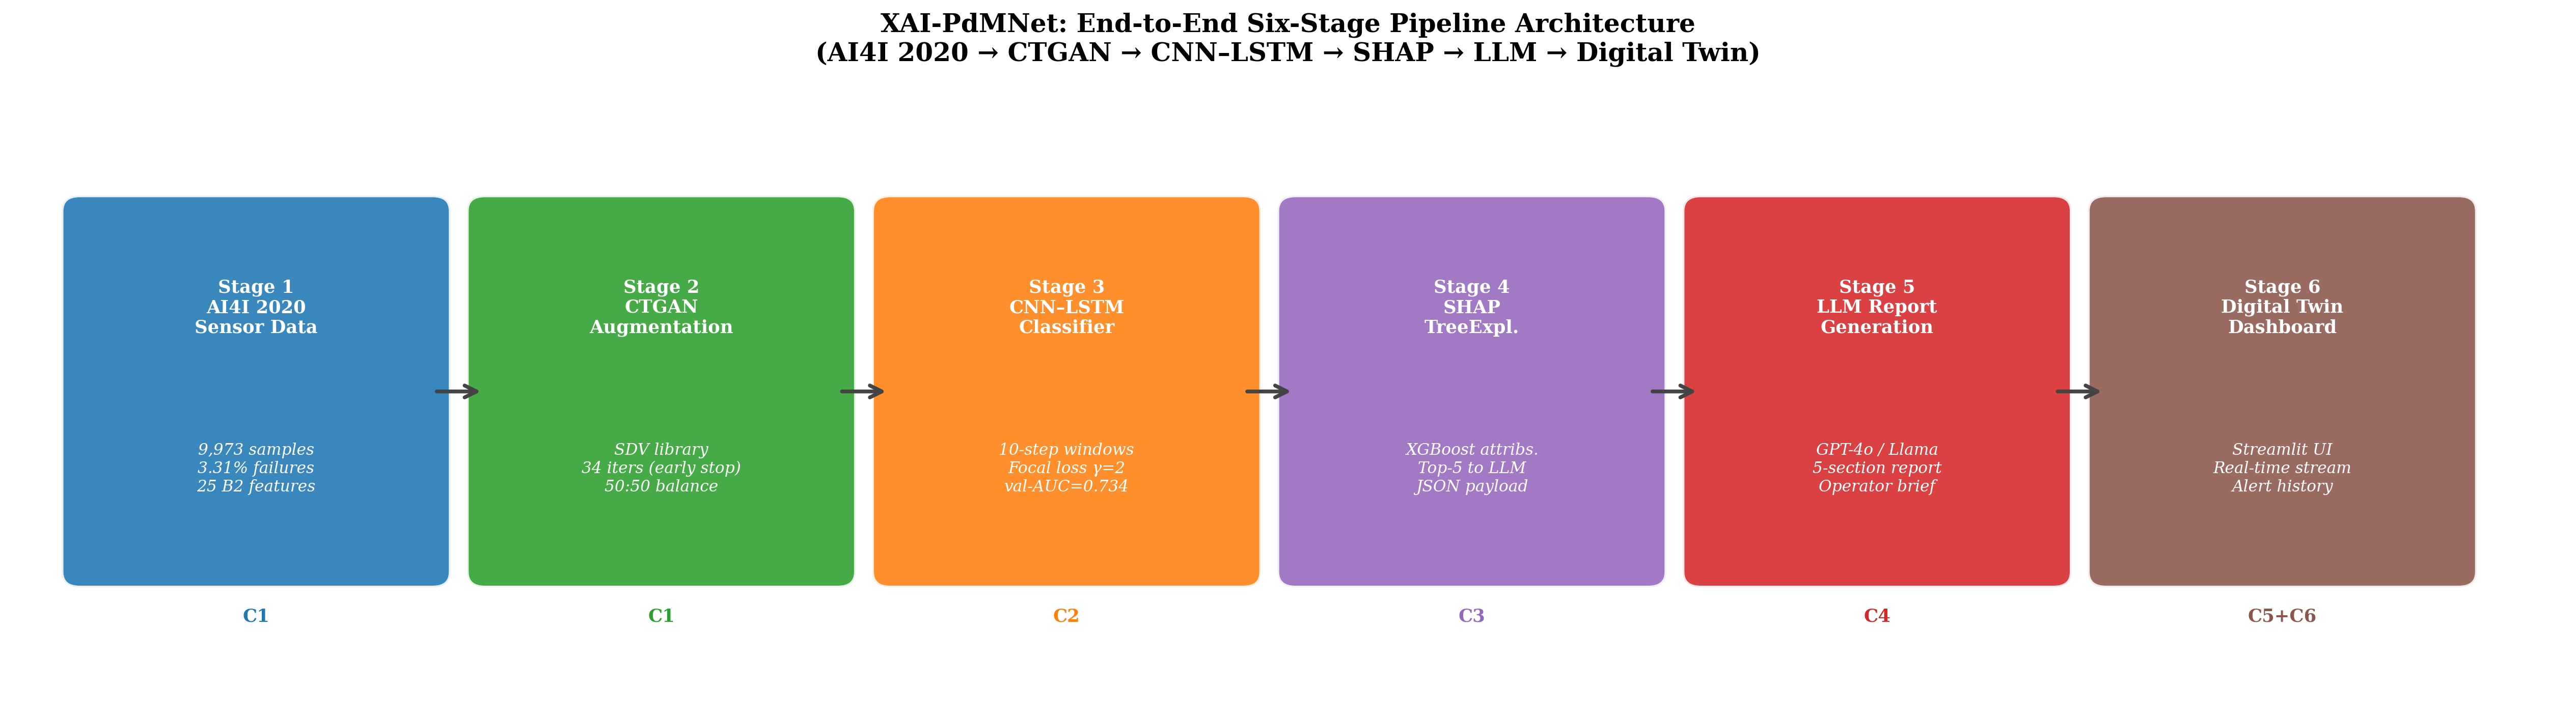
\includegraphics[width=\figfull]{fig1_pipeline.png}
\caption{XAI-PdMNet-Bench six-stage end-to-end pipeline architecture.\label{fig:pipeline}}
\end{figure}

Three design principles distinguish the framework:
\textit{leakage safety} (all target-derived columns excluded),
\textit{evaluation rigour} (shared imbalanced held-out test,
$n{=}1{,}993$), and \textit{human-centred interpretability}
(attribution plus structured operator report
\citep{ref-industry50-human2024,ref-xai-smart-mfg2025}).

\subsection{Pipeline Description}

The pipeline begins with sensor data ingestion and leakage-safe
feature construction.
After removing 27~internally inconsistent rows from
AI4I~2020~\citep{ref-ai4i2020}, 9{,}973~usable observations remain
(330~failure events, 3.31\%).
All five failure indicator sub-columns and identifier fields are
discarded (Section~\ref{sec:rw}), and 17~physically motivated
interaction features are appended to the five raw sensor channels,
yielding a 25-dimensional feature matrix
(Table~\ref{tab:features}).

The second stage addresses the class imbalance
(Section~\ref{sec:math}) through a CTGAN-based augmentation
audit \citep{ref-ctgan-original}.
A conditional generator is trained on the approximately
265~failure-class training rows and used to synthesise additional
failure samples until the augmented training set reaches a balanced
50:50 ratio.
Before any synthetic sample is admitted to training, its marginal
distributional fidelity is verified through Kolmogorov--Smirnov
goodness-of-fit tests on all 25 features, grounding augmentation in
statistical evidence rather than in optimistic assumptions.

Two parallel classification tracks share the held-out test set: a
tabular track (LR, RF, HGB, XGBoost) operating on the 25-feature
vector, and a temporal track (CNN--LSTM on ten-step sliding windows
with focal loss and class weighting). Because AI4I~2020 rows carry
no physical time ordering, the CNN--LSTM is treated as exploratory
(Sections~\ref{sec:math}--\ref{sec:method}).

SHAP TreeExplainer \citep{ref-shap-lundberg} computes exact Shapley
attributions for XGBoost predictions; the top-5 features populate a
deterministic five-section operator report (operator brief,
technician work order, safety escalation, manager summary,
30-minute checklist). Live LLM generation is future work
(Section~\ref{sec:conc}). A Streamlit dashboard
\citep{ref-digital-twin-pdm2024} closes the human--AI loop.
Algorithms~1 and~2 formalise the complete pipeline.

\begin{table}[H]
\centering
\begin{minipage}[t]{0.48\textwidth}
\centering
\scriptsize
\setlength{\tabcolsep}{2pt}
\begin{tabular}{l}
\toprule
\textbf{Algorithm~1}~~Data Preparation \& Training \\ \midrule
\textbf{Input:} $\mathcal{D}_\text{raw}$ ($n=10{,}000$) \\
\textbf{Output:} Trained models $\{f_k\}_{k=1}^{5}$ \\[3pt]
\textit{// Stage 1: Leakage-safe feature construction} \\
~~1: Drop TWF, HDF, PWF, OSF, RNF columns \\
~~2: Drop UID, Product ID \\
~~3: Remove 27 inconsistent rows $\to$ $n=9{,}973$ \\
~~4: Engineer 17 interaction features $\to$ $\mathbf{X} \in \mathbb{R}^{n \times 25}$ \\[3pt]
\textit{// Stage 2: Split \& CTGAN augmentation} \\
~~5: Stratified split: 68\%/12\%/20\% \\
~~6: Train CTGAN on failure rows ($\approx$265) \\
~~7: Synthesise 6{,}286 failure samples \\
~~8: KS-test all 25 features ($\alpha=0.05$) \\
~~9: \textbf{if} any $p < 0.05$ \textbf{then} reject batch \\
10: Merge $\to$ $\mathcal{D}_\text{aug}$ ($n=13{,}102$, 50:50) \\[3pt]
\textit{// Stage 3: Multi-model training} \\
11: \textbf{for} $f_k \in$ \{LR, RF, HGB, XGB\} \textbf{do} \\
12: ~~~~Train $f_k$ on $\mathcal{D}_\text{aug}$ (tabular) \\
13: \textbf{end for} \\
14: Reshape $\to$ sliding windows ($T$=10, stride=1) \\
15: Train CNN--LSTM with focal loss \\
16: Tune $\tau^*=\arg\max_\tau F_1(\mathcal{D}_\text{val})$ \\
\bottomrule
\end{tabular}
\end{minipage}\hfill
\begin{minipage}[t]{0.48\textwidth}
\centering
\scriptsize
\setlength{\tabcolsep}{2pt}
\begin{tabular}{l}
\toprule
\textbf{Algorithm~2}~~Evaluation \& Reporting \\ \midrule
\textbf{Input:} Trained $\{f_k\}$, $\mathcal{D}_\text{test}$ ($n=1{,}993$) \\
\textbf{Output:} Metrics, SHAP ranking, operator report \\[3pt]
\textit{// Stage 4: Held-out evaluation} \\
~~1: \textbf{for} $f_k \in$ \{LR, RF, HGB, XGB, CNN-LSTM\} \\
~~2: ~~~~$\hat{y}_k = f_k(\mathcal{D}_\text{test})$ \\
~~3: ~~~~Compute Acc, Prec, Rec, F1, AUC \\
~~4: \textbf{end for} \\
~~5: Select $f^* = \arg\max_k \text{PR-AUC}(f_k)$ \\[3pt]
\textit{// Stage 5: SHAP attribution} \\
~~6: Apply TreeExplainer to XGBoost on $\mathcal{D}_\text{test}$ \\
~~7: \textbf{for} each test row $i$: mean $|\phi_{i,j}|$ over trees \\
~~8: ~~$\bar{\phi}_j = \frac{1}{N_\text{test}}\sum_i |\phi_{i,j}|$ \\
~~9: (optional: GradientExplainer on CNN--LSTM for secondary analysis) \\
10: Rank features by $\bar{\phi}_j$ \\
11: Select top-$K=5$ $\to$ JSON payload \\[3pt]
\textit{// Stage 6: Operator report generation} \\
12: Pass payload to deterministic template \\
13: Generate 5-section maintenance report (template-based) \\
14: \textbf{return} metrics, $\{\bar{\phi}_j\}$, report \\
\bottomrule
\end{tabular}
\end{minipage}
\end{table}

%%%%%%%%%%%%%%%%%%%%%%%%%%%%%%%%%%%%%%%%%%
\section{Mathematical Problem Formulation}
\label{sec:math}

This section provides the complete mathematical foundation of the
XAI-PdMNet-Bench framework, covering the fault classification
objective, the class imbalance compensation strategy, the
convolutional--recurrent architecture, and the SHAP attribution
formulation.
All notation is introduced where first used and is consistent
throughout the remainder of the paper.

\subsection{Fault Classification, Class Imbalance, and Imbalance
Compensation}

\textbf{Problem statement.}
Let $\mathcal{D} = \{(\mathbf{x}_i, y_i)\}_{i=1}^{N}$ denote the
labelled sensor dataset, where
$\mathbf{x}_i \in \mathbb{R}^{d}$ ($d = 25$) is the leakage-safe
feature vector for observation $i$ and $y_i \in \{0, 1\}$ is the
binary machine-failure label.
The goal is to learn a predictor
$f_\theta: \mathbb{R}^{d} \to [0,1]$ parameterised by $\theta$
such that $\hat{p}_i = f_\theta(\mathbf{x}_i)$ estimates
$\Pr(y_i = 1 \mid \mathbf{x}_i)$ and the expected loss is minimised:

\begin{linenomath}
\begin{equation}
\theta^* = \operatorname*{arg\,min}_{\theta}\;
  \mathbb{E}_{(\mathbf{x},y)\sim\mathcal{D}}
  \bigl[\mathcal{L}\!\left(f_\theta(\mathbf{x}),\,y\right)\bigr].
\label{eq:objective}
\end{equation}
\end{linenomath}

\noindent A hard prediction is obtained by thresholding at a
tuned decision boundary $\tau^*$:
$\hat{y}_i = \mathbb{1}[\hat{p}_i \geq \tau^*]$,
where $\tau^*$ is selected on the validation set by maximising the
F1-score:

\begin{linenomath}
\begin{equation}
\tau^* = \operatorname*{arg\,max}_{\tau \in (0,1)}\;
  F_1\!\left(y_\text{val},\,
  \mathbb{1}[\hat{p}_\text{val} \geq \tau]\right).
\label{eq:threshold}
\end{equation}
\end{linenomath}

\textbf{Class imbalance.}
The class prior probabilities are $\pi_0 = \Pr(y{=}0) = 0.9669$
and $\pi_1 = \Pr(y{=}1) = 0.0331$, giving an imbalance ratio
$\rho = \pi_0/\pi_1 = 29.25$.
A naïve maximum-likelihood classifier predicts the majority class
for all inputs, achieving accuracy $\pi_0 = 96.69\%$ but recall
$= 0$, which is operationally useless for fault detection.
Three complementary mechanisms are applied to correct this bias.

\textbf{Mechanism 1 — Generative augmentation (CTGAN).}
A Conditional Tabular GAN \citep{ref-ctgan-original} is trained on
the minority-class training rows.
The generator $G: \mathbb{R}^{n_z} \times \{0,1\} \to \mathbb{R}^d$
maps a Gaussian noise vector $\mathbf{z} \sim \mathcal{N}(\mathbf{0},
\mathbf{I})$ and a class condition $c = 1$ to a synthetic
failure-class feature vector:

\begin{linenomath}
\begin{equation}
\tilde{\mathbf{x}} = G(\mathbf{z},\, c{=}1),
\quad \mathbf{z} \sim \mathcal{N}(\mathbf{0}, \mathbf{I}_{n_z}).
\label{eq:ctgan}
\end{equation}
\end{linenomath}

\noindent Synthetic samples are generated until the augmented
training set reaches a 50:50 class balance
($\tilde{\rho} = 1$).
Before training, each synthetic feature $j$ is validated by a
Kolmogorov--Smirnov test against the real training distribution:
$D_j = \sup_x|F_j^{\text{real}}(x) - F_j^{\text{synth}}(x)|$,
with the null hypothesis of identical distributions retained if
$D_j$ does not exceed the critical value at $\alpha = 0.05$.

\textbf{Mechanism 2 — Cost-sensitive class weighting.}
Even after augmentation, residual imbalance in the per-batch sample
distribution is addressed by scaling the loss contribution of each
class $c \in \{0,1\}$ by an inverse-frequency weight:

\begin{linenomath}
\begin{equation}
w_c = \frac{N_\text{aug}}{K \cdot N_c^{\text{aug}}},
\label{eq:classweight}
\end{equation}
\end{linenomath}

\noindent where $N_\text{aug}$ is the total augmented training set
size, $K = 2$ is the number of classes, and $N_c^{\text{aug}}$ is
the number of samples from class $c$ after augmentation.

\textbf{Mechanism 3 — Focal loss.}
Standard binary cross-entropy assigns equal gradient weight to easy
and hard examples.
Focal loss \citep{ref-focal-loss} modulates the per-sample loss by a
factor $(1-\hat{p}_t)^\gamma$ that down-weights confident correct
predictions, focusing training on misclassified boundary cases:

\begin{linenomath}
\begin{equation}
\mathcal{L}_\text{FL}(\hat{p}_t, y) =
  -\alpha_t\,(1-\hat{p}_t)^{\gamma}\,\log(\hat{p}_t),
\label{eq:focal}
\end{equation}
\end{linenomath}

\noindent where $\hat{p}_t = \hat{p}$ if $y = 1$ and
$\hat{p}_t = 1 - \hat{p}$ if $y = 0$;
$\alpha_t = \alpha$ for the positive class and
$\alpha_t = 1 - \alpha$ for the negative class.
In this work, $\gamma = 2.0$ and $\alpha = 0.75$.
As shown in Section~\ref{sec:discuss_cnnlstm}, the simultaneous
application of all three mechanisms constitutes triple imbalance
compensation, which compresses output probabilities toward small
magnitudes, a documented side-effect of focal loss
\citep{ref-calibration-focal2020}, and necessitates post-hoc
calibration before deployment-level threshold claims can be made.

\subsection{Feature Standardisation, Temporal Windowing, and
CNN--LSTM Architecture}

\textbf{Feature standardisation.}
All $d = 25$ features are standardised using training-set
statistics to prevent information leakage from the validation or
test splits.
For feature $j$ and training set of size $N_\text{tr}$:

\begin{linenomath}
\begin{equation}
\hat{x}_{i,j} = \frac{x_{i,j} - \hat{\mu}_j}{\hat{\sigma}_j},
\quad
\hat{\mu}_j = \frac{1}{N_\text{tr}}\sum_{i=1}^{N_\text{tr}} x_{i,j},
\quad
\hat{\sigma}_j = \sqrt{\frac{1}{N_\text{tr}{-}1}
  \sum_{i=1}^{N_\text{tr}}(x_{i,j} - \hat{\mu}_j)^2}.
\label{eq:scaler}
\end{equation}
\end{linenomath}

\textbf{Sliding-window encoding.}
The standardised feature matrix
$\hat{\mathbf{X}} \in \mathbb{R}^{N \times d}$ is segmented into
overlapping tensors of length $T = 10$ with stride 1.
The window ending at index $t$ and its associated label are:

\begin{linenomath}
\begin{equation}
\mathbf{W}_t = \bigl[\hat{\mathbf{x}}_{t-T+1},\;
  \hat{\mathbf{x}}_{t-T+2},\;\ldots,\;
  \hat{\mathbf{x}}_{t}\bigr]
\in \mathbb{R}^{T \times d},
\qquad
y_t^{(w)} = y_t.
\label{eq:window}
\end{equation}
\end{linenomath}

\noindent This yields $N - T + 1 = 9{,}964$ window--label pairs.
The CNN--LSTM predicts $\hat{p}_t = f_\theta(\mathbf{W}_t)$ for
each window.

\textbf{Conv1D feature extraction.}
The first stage of the CNN--LSTM applies two stacked
one-dimensional convolutional layers.
For input tensor $\mathbf{W}_t$, filter bank $k$ of width $K_f$,
and filter weights $\mathbf{w}^{(k)} \in \mathbb{R}^{K_f \times d}$:

\begin{linenomath}
\begin{equation}
z_{t',k} = \text{ReLU}\!\left(
  \sum_{\tau=0}^{K_f-1} \mathbf{W}_t[t'+\tau,\,:]
  \cdot \mathbf{w}^{(k)}[\tau,\,:] + b_k
\right),
\label{eq:conv1d}
\end{equation}
\end{linenomath}

\noindent where $t'$ indexes the output position after convolution,
and $b_k$ is the bias.
The first Conv1D layer uses 64~filters of width~3; the second uses
32~filters of width~3, followed by MaxPool1D with pool size~2.

\textbf{LSTM temporal modelling.}
The convolutional output sequence is processed by two stacked LSTM
layers.
At each timestep $t'$, given input $\mathbf{z}_{t'}$ and previous
hidden state $\mathbf{h}_{t'-1}$, the LSTM computes:

\begin{linenomath}
\begin{align}
\mathbf{f}_{t'} &= \sigma\!\left(
  \mathbf{W}_f[\mathbf{h}_{t'-1};\mathbf{z}_{t'}] + \mathbf{b}_f
  \right), \label{eq:lstm-f} \\
\mathbf{i}_{t'} &= \sigma\!\left(
  \mathbf{W}_i[\mathbf{h}_{t'-1};\mathbf{z}_{t'}] + \mathbf{b}_i
  \right), \label{eq:lstm-i} \\
\mathbf{g}_{t'} &= \tanh\!\left(
  \mathbf{W}_g[\mathbf{h}_{t'-1};\mathbf{z}_{t'}] + \mathbf{b}_g
  \right), \label{eq:lstm-g} \\
\mathbf{o}_{t'} &= \sigma\!\left(
  \mathbf{W}_o[\mathbf{h}_{t'-1};\mathbf{z}_{t'}] + \mathbf{b}_o
  \right), \label{eq:lstm-o} \\
\mathbf{c}_{t'} &= \mathbf{f}_{t'} \odot \mathbf{c}_{t'-1}
  + \mathbf{i}_{t'} \odot \mathbf{g}_{t'}, \label{eq:lstm-c} \\
\mathbf{h}_{t'} &= \mathbf{o}_{t'} \odot
  \tanh(\mathbf{c}_{t'}), \label{eq:lstm-h}
\end{align}
\end{linenomath}

\noindent where $\mathbf{f}$, $\mathbf{i}$, $\mathbf{g}$,
$\mathbf{o}$ are the forget gate, input gate, cell candidate, and
output gate activations respectively; $\odot$ denotes element-wise
multiplication; and $[\,;\,]$ denotes vector concatenation.
The first LSTM layer (64~units) returns the full sequence; the
second (32~units) returns the final hidden state
$\mathbf{h}_{T'}$ after dropout regularisation.

\textbf{Classification head and full composition.}
The final hidden state is projected to a scalar fault probability
through a Dense(16)--ReLU--Dense(1)--Sigmoid head:

\begin{linenomath}
\begin{equation}
f_\theta(\mathbf{W}_t)
  = \sigma\!\left(\mathbf{w}_h^\top\,
    g_\text{LSTM}\!\left(g_\text{CNN}(\mathbf{W}_t)\right) + b_h
  \right) \in [0,1],
\label{eq:composition}
\end{equation}
\end{linenomath}

\noindent where $\sigma(x) = (1 + e^{-x})^{-1}$ is the sigmoid
activation, $g_\text{CNN}$ denotes the Conv1D--MaxPool sub-network,
and $g_\text{LSTM}$ denotes the stacked LSTM sub-network.

\subsection{SHAP Attribution and End-to-End Pipeline}

\textbf{SHAP local accuracy.}
For a trained model $f_\theta$ and an input
$\mathbf{W}_t \in \mathbb{R}^{T \times d}$, the SHAP
GradientExplainer \citep{ref-shap-lundberg} assigns an attribution
$\phi_{j,\tau}(\mathbf{W}_t)$ to each feature $j$ at each
timestep $\tau$.
The attributions satisfy the local accuracy axiom:

\begin{linenomath}
\begin{equation}
f_\theta(\mathbf{W}_t) = \phi_0 +
  \sum_{j=1}^{d} \sum_{\tau=1}^{T}
  \phi_{j,\tau}(\mathbf{W}_t),
\label{eq:shap-local}
\end{equation}
\end{linenomath}

\noindent where $\phi_0 = \mathbb{E}_{\mathbf{W}}[f_\theta(\mathbf{W})]$
is the expected model output (baseline).

\textbf{Global feature importance.}
To obtain a dataset-level importance score for each of the $d$
features, attributions are first averaged over the $T$ timesteps
of each window and then averaged in absolute value over all
$N_\text{test}$ test instances:

\begin{linenomath}
\begin{equation}
\bar{\phi}_j =
  \frac{1}{N_\text{test}}
  \sum_{i=1}^{N_\text{test}}
  \left\lvert
    \frac{1}{T}\sum_{\tau=1}^{T}
    \phi_{j,\tau}(\mathbf{W}_i)
  \right\rvert.
\label{eq:shap-agg}
\end{equation}
\end{linenomath}

\noindent The top-$K$ features by $\bar{\phi}_j$ (with $K = 5$
in this work, computed from TreeExplainer for XGBoost in the primary
deployment path) are selected as the dominant fault drivers and
packaged as a structured JSON payload for the operator report.

\textbf{SHAP TreeExplainer for ensemble backbones.}
For gradient-boosted tree models (our strongest classifier, XGBoost),
SHAP TreeExplainer yields exact additive feature attributions without
approximation (unlike GradientExplainer for neural networks) by
enumerating coalition contributions inside each regression tree.
Global importance $\bar{\phi}_j$ averages mean absolute attributions
$\lvert\phi_{j,i}\rvert$ over held-out test rows $i$.
For the CNN--LSTM branch only, Equations~(\ref{eq:shap-local})--(\ref{eq:shap-agg})
with GradientExplainer over windowed inputs remain in effect for
comparison and ablation-style interpretability.

\textbf{End-to-end pipeline.}
The complete XAI-PdMNet-Bench transformation from a sensor window
to a structured maintenance report is expressed as the composite
function:

\begin{linenomath}
\begin{equation}
\mathcal{R} =
  \mathcal{F}_\text{report}\!\Bigl(
    \text{Top}_K\!\left(\bar{\boldsymbol{\phi}}\right),\;
    \hat{p},\;
    \tau
  \Bigr),
\label{eq:pipeline}
\end{equation}
\end{linenomath}

\noindent where $\mathcal{R}$ is the five-section operator
maintenance report,
$\bar{\boldsymbol{\phi}} \in \mathbb{R}^d$ is the global SHAP
importance vector (primary: TreeExplainer on XGBoost for
$\mathbf{x}$; secondary: GradientExplainer aggregated over windows
for CNN--LSTM via Equation~\ref{eq:shap-agg}),
$\text{Top}_K(\cdot)$ selects the $K$ entries with the largest
magnitude,
$\hat{p}$ is the backbone fault probability from the selected
classifier (production default: $\hat{p} = f_\text{XGB}(\mathbf{x})$
at $\tau = 0.50$; CNN--LSTM uses $\tau^* = 0.31$ from Equation~\ref{eq:threshold}),
and $\tau$ denotes the operating threshold.
This formulation makes explicit that the operator-facing output
is determined by three inputs: the model's discriminative
probability, the physical features that drove that probability,
and the operating decision boundary, closing the human--AI
communication loop required by Industry~5.0.

%%%%%%%%%%%%%%%%%%%%%%%%%%%%%%%%%%%%%%%%%%
\section{Methodology}
\label{sec:method}

\subsection{Dataset, Preprocessing, and Experimental Configuration}

\textbf{Dataset.}
All experiments use the AI4I~2020 predictive maintenance dataset
\citep{ref-ai4i2020} (UCI ML Repository, ID: 601,
DOI:~10.24432/C5HS5C, licence: CC~BY~4.0), a synthetic milling
machine simulation recording five continuous process sensor channels
(air temperature, process temperature, rotational speed, torque, tool
wear), a three-class product quality indicator, and a binary
machine-failure label.
Following removal of 27~rows with internally inconsistent failure
labels, 9{,}973~usable observations remain, of which 330~(3.31\%)
are failure events (imbalance ratio $\rho = 29.25$; Section~\ref{sec:math}).
AI4I~2020 is generated row-by-row by a
known mathematical simulation formula; consecutive rows do not
constitute a physical machine timeline.
All temporal modelling is therefore treated as exploratory, and
claims of temporal predictive benefit require validation on
physically ordered industrial sensor logs.

\textbf{Feature construction.}
As detailed in Section~\ref{sec:model}, all five failure indicator
sub-columns and identifier fields are excluded to prevent label
leakage.
The five raw sensor channels are augmented with 17~physically
motivated interaction and transformation features (e.g., RPM~$\times$~tool
wear for cumulative mechanical stress, torque~$\times$~RPM for
instantaneous power), yielding $\mathbf{x} \in \mathbb{R}^{25}$.
The complete feature set is listed in Table~\ref{tab:features}.

\begin{table}[H]
\caption{Process-informed feature set used for classification
($d = 25$). All five failure indicator columns and identifier fields
are excluded to prevent label leakage.\label{tab:features}}
\centering
\mdpitablefont
\begin{tabularx}{\textwidth}{llX}
\toprule
\textbf{Feature} & \textbf{Type} & \textbf{Physical motivation} \\
\midrule
Air temperature (K)             & Raw sensor  & Ambient thermal load; linked to heat-dissipation risk \\
Process temperature (K)         & Raw sensor  & Cutting-zone temperature; primary HDF indicator \\
Rotational speed (rpm)          & Raw sensor  & Spindle speed; high values increase mechanical stress \\
Torque (Nm)                     & Raw sensor  & Cutting resistance; combined with wear drives OSF \\
Tool wear (min)                 & Raw sensor  & Cumulative degradation; primary TWF and OSF driver \\
Type L / Type M / Type H        & Encoded     & One-hot product quality tier; affects wear accumulation rate \\
\midrule
Torque $\times$ RPM             & Engineered  & Instantaneous mechanical power (W); drives PWF and HDF \\
RPM / Torque                    & Engineered  & Speed--load ratio; indicates overloading conditions \\
Torque $\times$ Tool wear       & Engineered  & Overload--degradation interaction; primary OSF proxy \\
RPM $\times$ Tool wear          & Engineered  & Cumulative mechanical stress; primary TWF proxy \\
Power / Tool wear               & Engineered  & Normalised load per unit wear; captures accelerating failure \\
Process temp $-$ Air temp (K)   & Engineered  & Thermal gradient; HDF triggered when gap $< 8.6$~K at high RPM \\
Process temp / Air temp         & Engineered  & Thermal efficiency ratio \\
$\log(1 + \text{Torque})$       & Engineered  & Variance-stabilising transform for heavy-tailed torque \\
$\log(1 + \text{RPM})$          & Engineered  & Variance-stabilising transform for rotational speed \\
$\log(1 + \text{Tool wear})$    & Engineered  & Compresses long-tail wear distribution \\
$\log(1 + \text{Power proxy})$  & Engineered  & Log-scaled mechanical power \\
Normalised tool wear            & Engineered  & Min-max scaled wear for feature comparability \\
Process temp $\times$ Torque    & Engineered  & Thermal-mechanical coupling load \\
$1 / \text{Air temp}$           & Engineered  & Inverse thermal load; monotone feature complement \\
$(\Delta\text{temp})^2$         & Engineered  & Nonlinear thermal gradient sensitivity \\
$(\Delta\text{temp}) / \text{Wear}$ & Engineered & Thermal stress per unit degradation \\
\bottomrule
\end{tabularx}
\end{table}

\textbf{Data partitioning and normalisation.}
The 9{,}973 observations are divided into training (68\%),
validation (12\%), and held-out test (20\%) splits using stratified
random sampling with seed~42, preserving the 3.31\% minority-class
proportion in all three partitions.
This yields 6{,}775 training, 1{,}196 validation, and 1{,}993 test
samples; the test set contains 66~failure and 1{,}927~normal
instances.
All features are standardised using zero-mean, unit-variance
normalisation (Equation~\ref{eq:scaler}) fitted exclusively on the
training split; the same statistics are applied to validation and
test sets without refitting to prevent normalisation leakage.

\textbf{Sensor distributions and failure mode analysis.}
Figure~\ref{fig:eda_panel} shows the sensor value distributions
separated by class.
RPM exhibits a statistically significant downward mean shift of
$-148$~rpm in failure events, torque increases by $+6$~Nm, and tool
wear shows the largest shift of $+61$~min, directly explaining why
the RPM--wear and power-proxy interaction terms become dominant SHAP
features.
Table~\ref{tab:failmodes} details the per-mode failure counts;
Heat Dissipation Failure (115~events, 34.8\%) is the most frequent
mode, followed by Overstrain (98~events, 29.7\%) and Power Failure
(95~events, 28.8\%).
These distributions motivate the specific engineered features and
confirm that the 25-feature representation covers all four
deterministic failure mechanisms.

\begin{table}[H]
\caption{Failure mode distribution in AI4I~2020
($n_\text{fail} = 330$; 3 rows are multi-label).
All five failure indicator columns are excluded from classifier
inputs throughout this study.\label{tab:failmodes}}
\centering
\mdpitablefont
\begin{tabularx}{\textwidth}{lXcc}
\toprule
\textbf{Failure mode} & \textbf{Physical trigger condition} &
\textbf{Count} & \textbf{Share (\%)} \\
\midrule
Heat Dissipation (HDF) &
  Process--air temp gap $<$ 8.6~K at RPM $>$ 1380 & 115 & 34.8 \\
Overstrain (OSF) &
  Torque $\times$ wear $>$ quality-tier threshold & 98 & 29.7 \\
Power Failure (PWF) &
  Torque $\times$ RPM $\notin [3500,\,9000]$~W & 95 & 28.8 \\
Tool Wear (TWF) &
  Cumulative RPM $\times$ wear exceeds limit & 46 & 13.9 \\
Random (RNF) &
  Stochastic 0.1\% base rate & 18 & 5.5 \\
\bottomrule
\end{tabularx}
\end{table}

\begin{figure}[H]
\centering
\begin{minipage}[t]{0.48\textwidth}
\centering
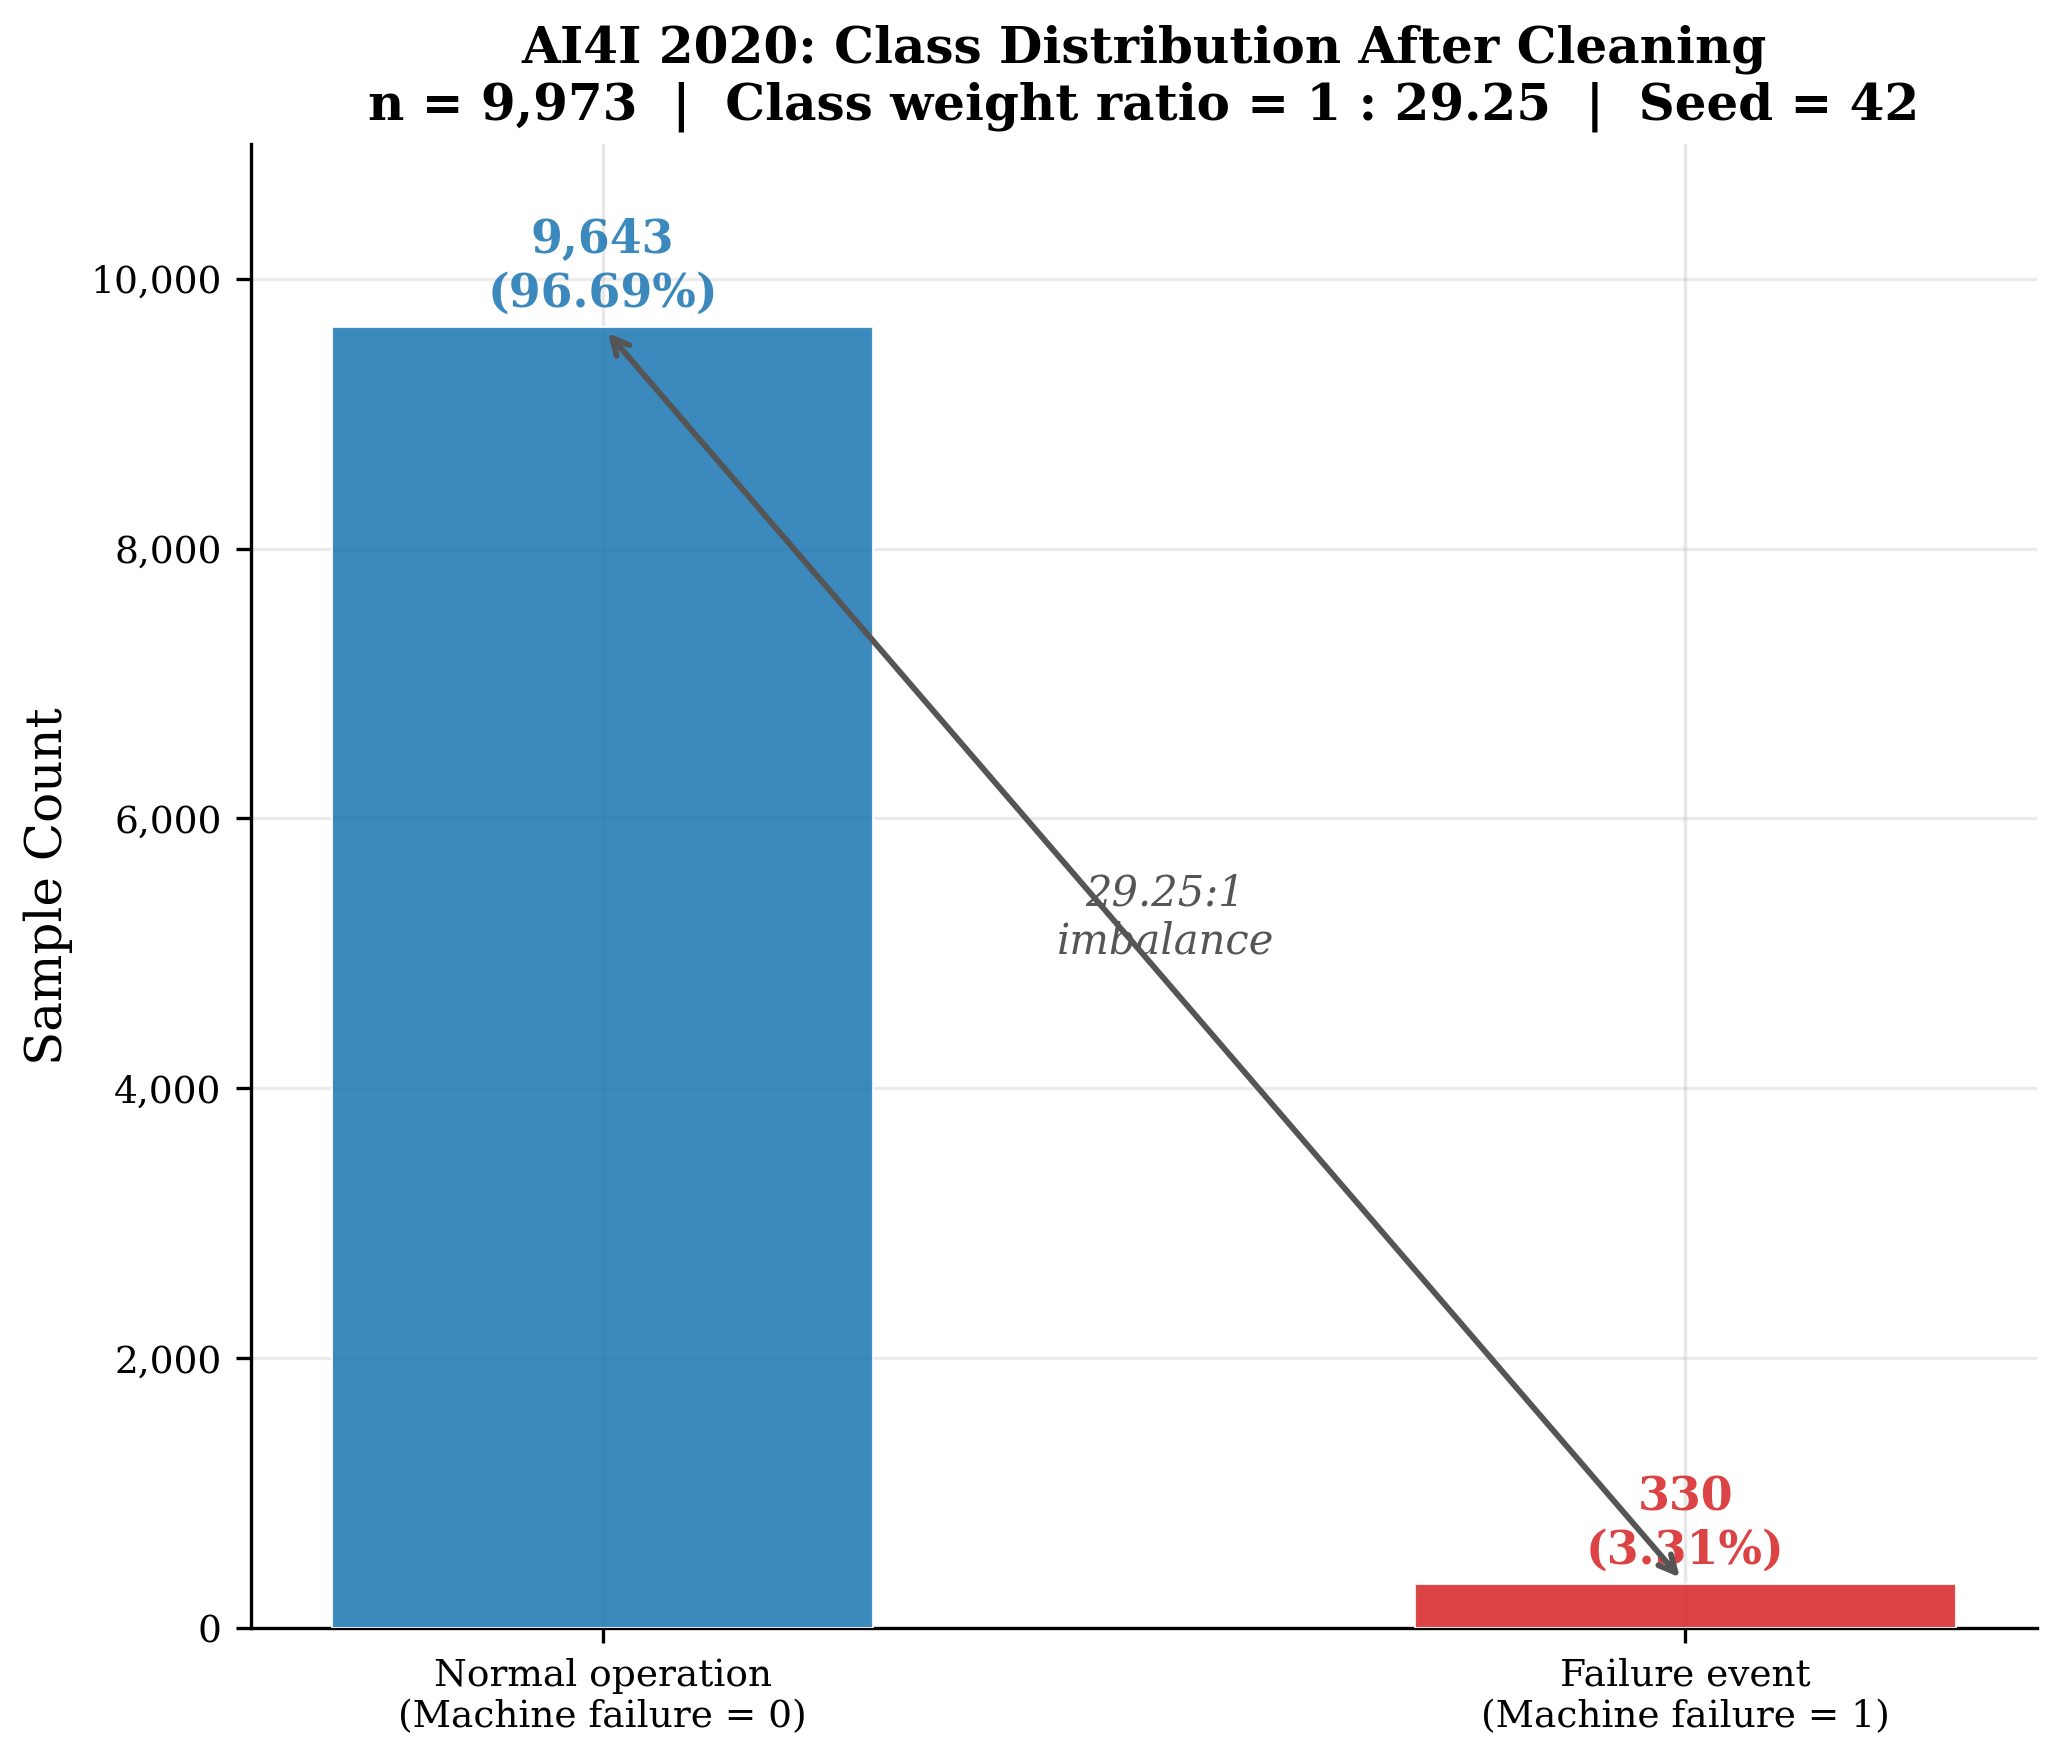
\includegraphics[width=\textwidth]{fig6a_class_distribution.png}
\end{minipage}\hfill
\begin{minipage}[t]{0.48\textwidth}
\centering
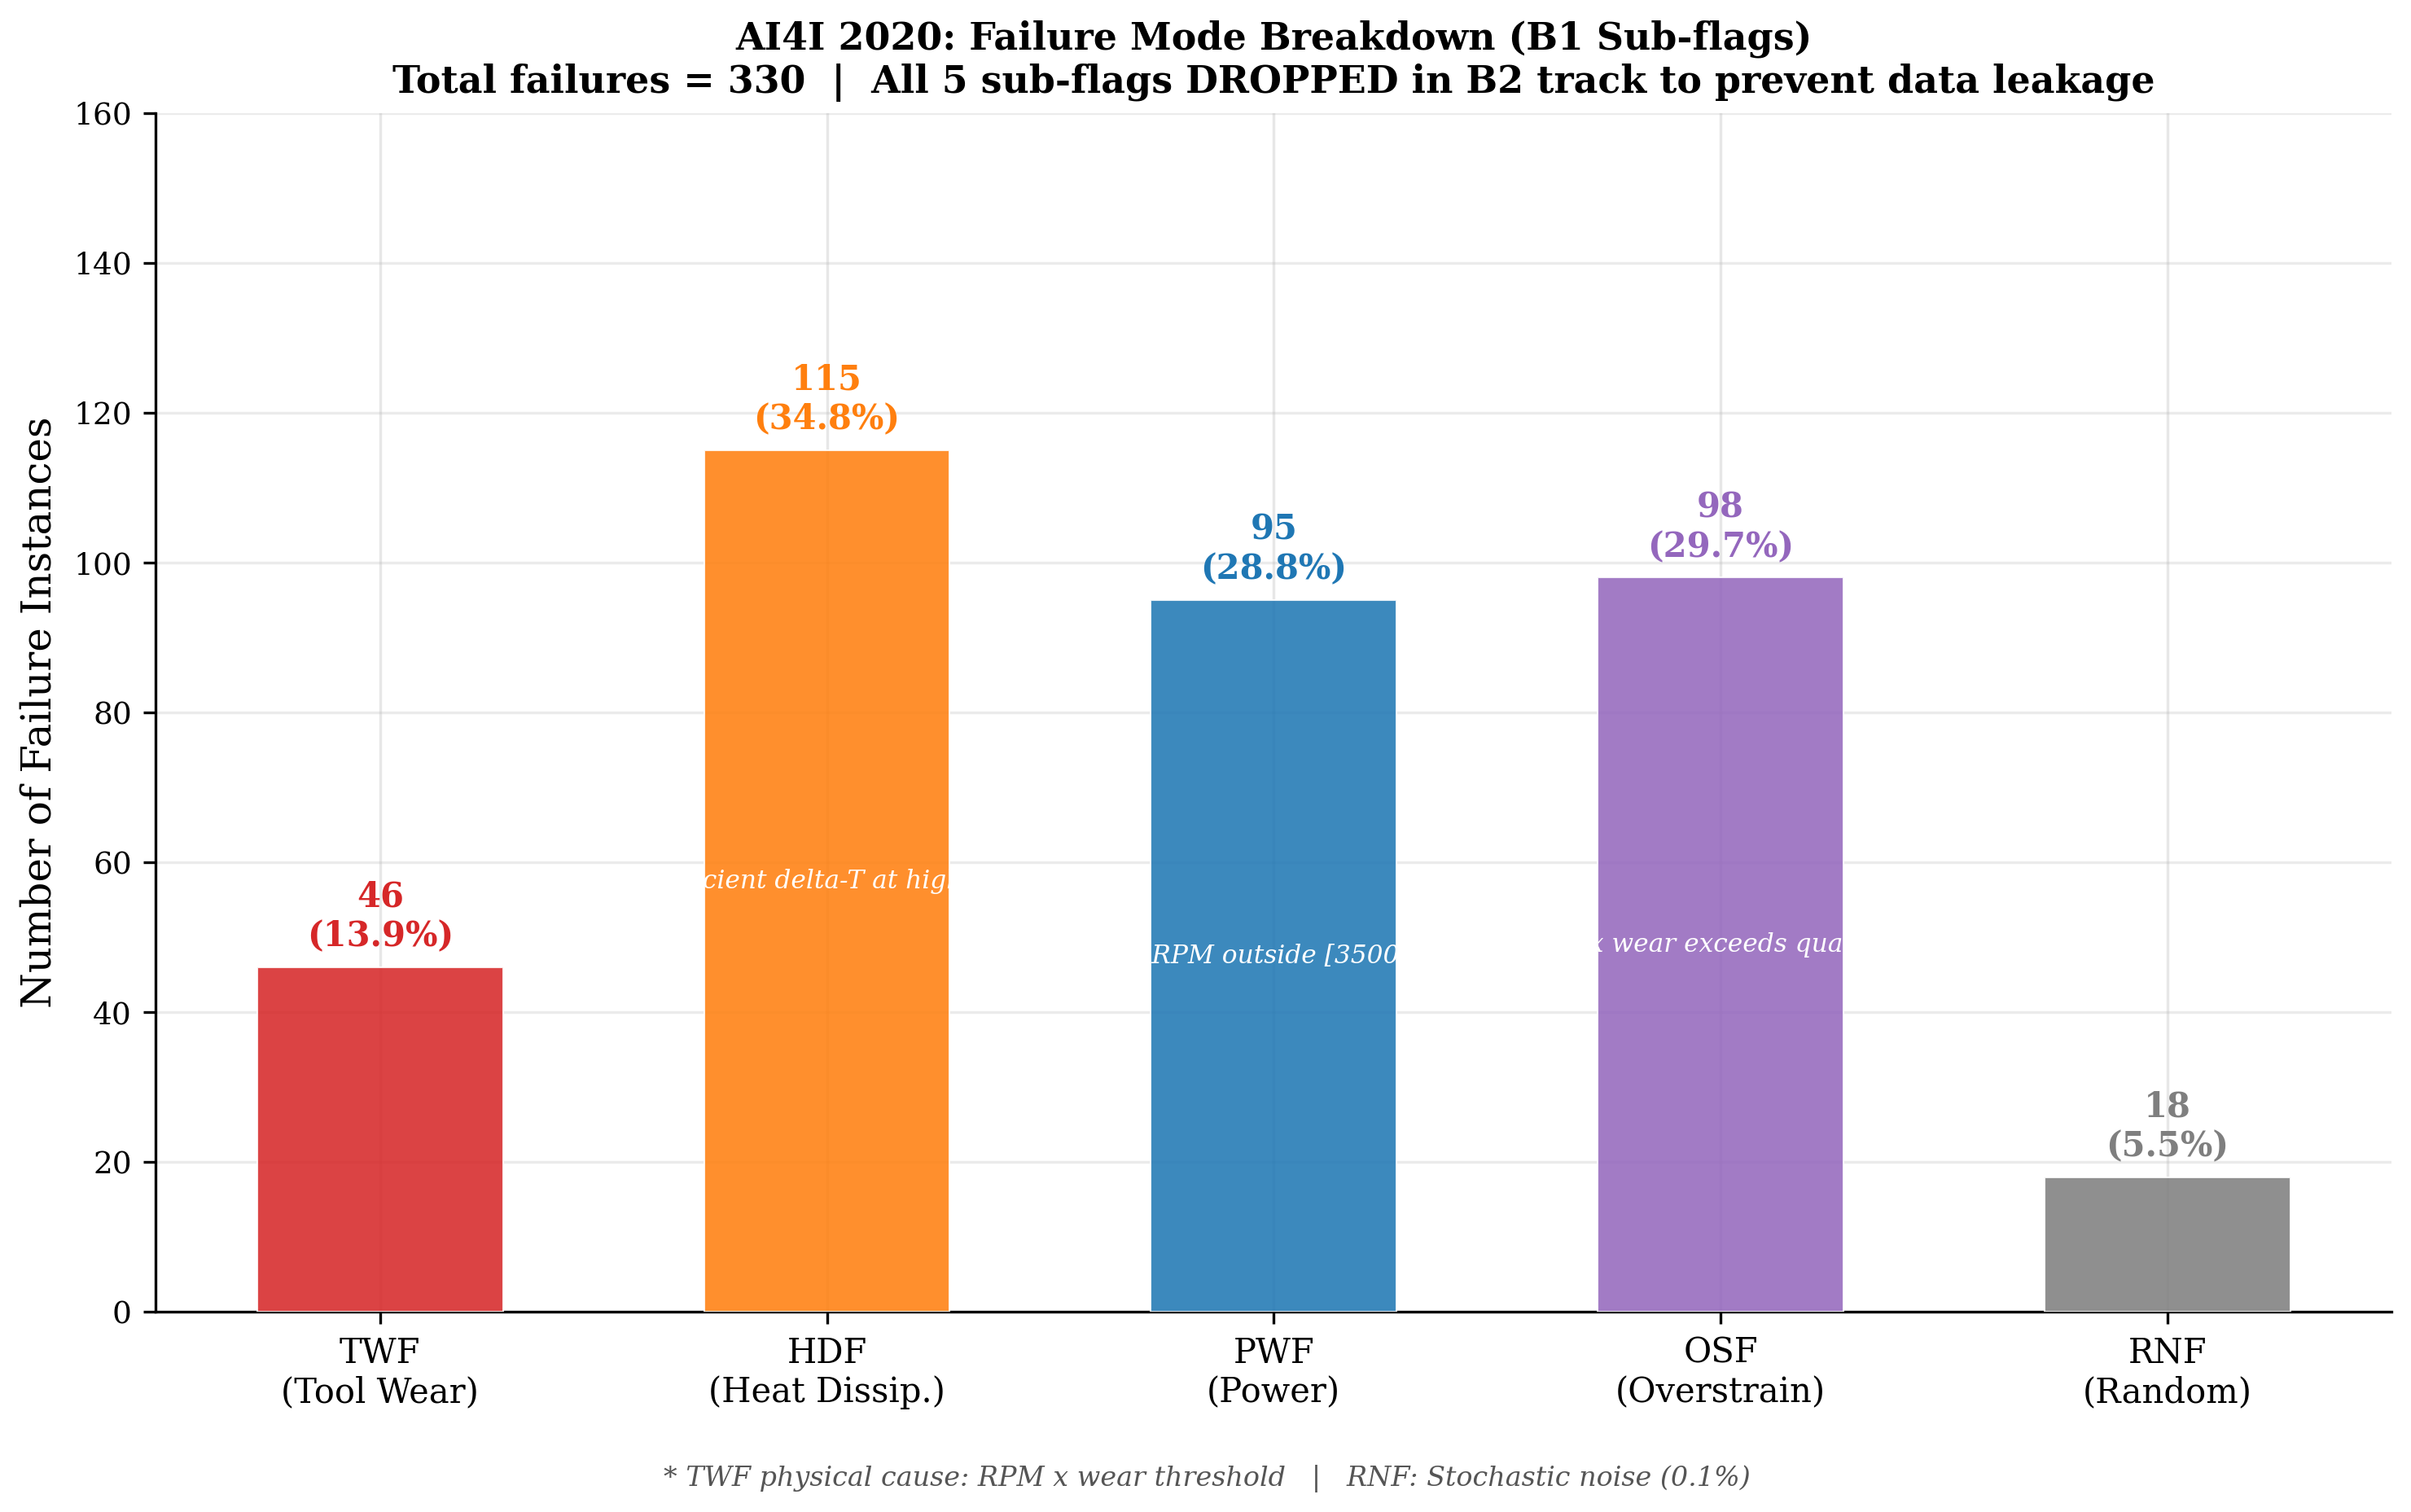
\includegraphics[width=\textwidth]{fig6c_failure_modes.png}
\end{minipage}

\vspace{6pt}

\begin{minipage}[t]{0.48\textwidth}
\centering
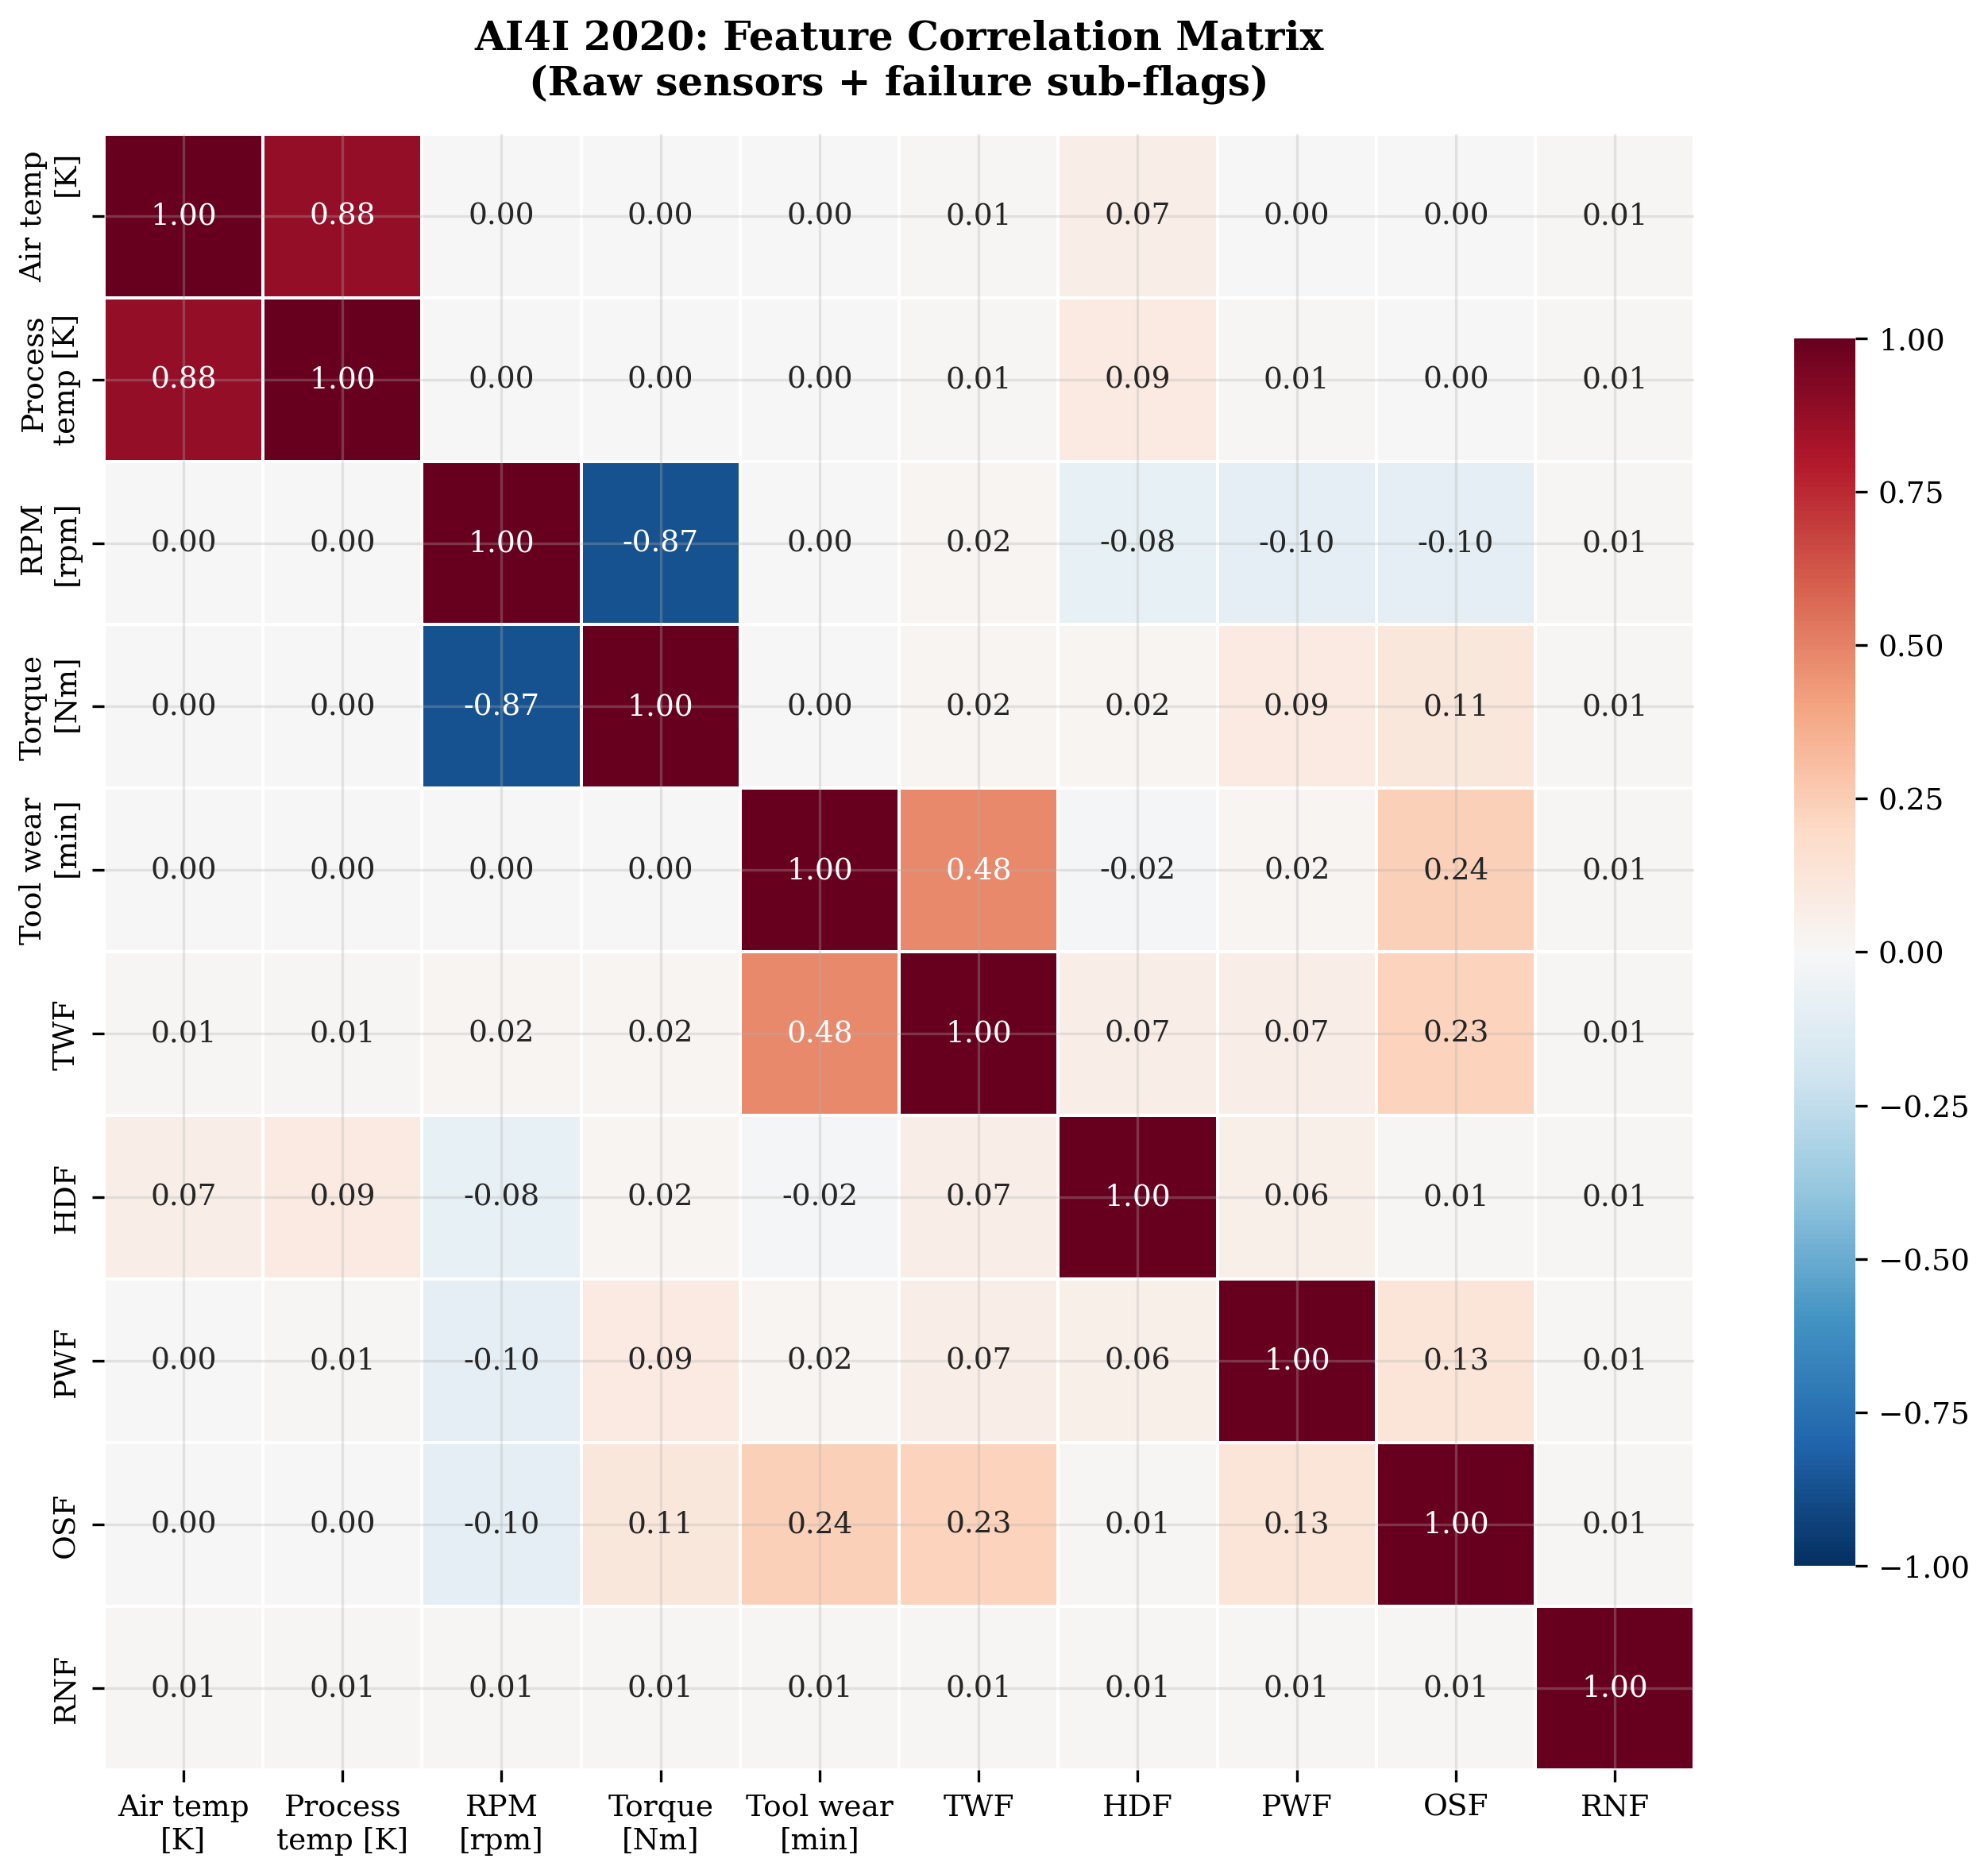
\includegraphics[width=\textwidth]{fig6b_correlation.png}
\end{minipage}\hfill
\begin{minipage}[t]{0.48\textwidth}
\centering
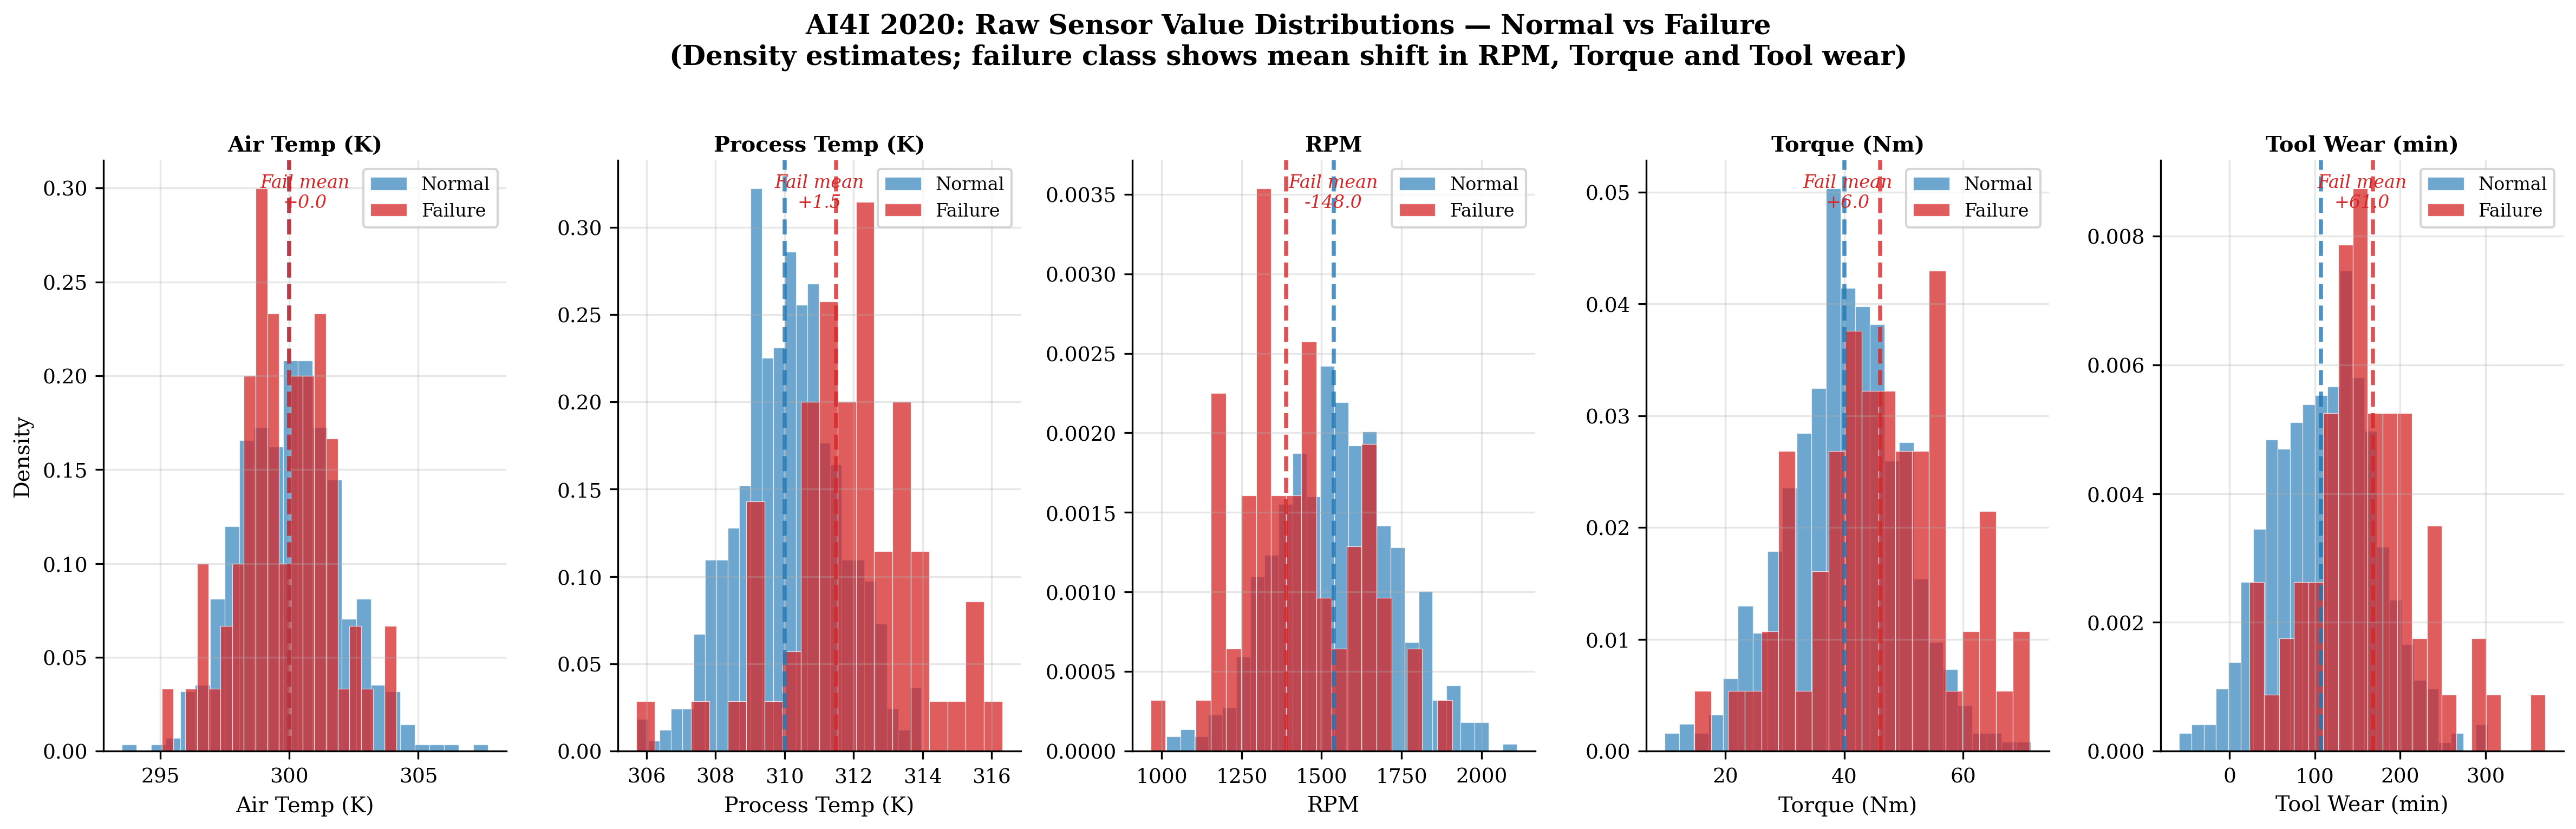
\includegraphics[width=\textwidth]{fig6d_sensor_distributions.png}
\end{minipage}
\caption{Exploratory data analysis of AI4I~2020: (a)~class distribution, (b)~failure mode counts, (c)~sensor correlation matrix, (d)~normal vs.\ failure distributions.\label{fig:eda_panel}}
\end{figure}

\textbf{Reproducibility.}
Table~\ref{tab:params} lists the complete experimental configuration.
All random number generators (NumPy, TensorFlow, scikit-learn, CTGAN)
are seeded with the same value (42) to ensure full deterministic
reproducibility.

\begin{table}[H]
\caption{Complete experimental configuration and software
environment.\label{tab:params}}
\centering
\mdpitablefont
\begin{tabularx}{\textwidth}{lX}
\toprule
\textbf{Configuration item} & \textbf{Value / version} \\
\midrule
\multicolumn{2}{l}{\textit{Hardware and software environment}} \\
Execution environment      & Google Colab Pro (GPU: NVIDIA Tesla T4, 16~GB) \\
Programming language       & Python 3.10 \\
Deep learning framework    & TensorFlow 2.15 / Keras \\
ML classifiers             & scikit-learn 1.3, XGBoost 2.0 \\
Generative augmentation    & SDV library v1.9 (CTGAN) \\
Explainability             & SHAP 0.45 (TreeExplainer + GradientExpl.) \\
Dashboard                  & Streamlit 1.35, Plotly 5.0 \\
Random seed                & 42 (all libraries) \\
\midrule
\multicolumn{2}{l}{\textit{Data partitioning}} \\
Train / validation / test split & 68\% / 12\% / 20\% (stratified, seed 42) \\
Training samples           & 6{,}775 (224 failures, 6{,}551 normal) \\
Validation samples         & 1{,}196 (40 failures, 1{,}156 normal) \\
Test samples               & 1{,}993 (66 failures, 1{,}927 normal) \\
\midrule
\multicolumn{2}{l}{\textit{CNN--LSTM training hyperparameters}} \\
Window length / stride     & 10 timesteps / 1 \\
Conv1D layers              & Conv1D(64, $k$=3, ReLU) $\to$ Conv1D(32, $k$=3, ReLU) $\to$ MaxPool1D(2) \\
LSTM layers                & LSTM(64, return\_seq=True) $\to$ Dropout(0.3) $\to$ LSTM(32) $\to$ Dropout(0.2) \\
Classification head        & Dense(16, ReLU) $\to$ Dense(1, sigmoid) \\
Loss function              & Focal loss ($\gamma = 2.0$, $\alpha = 0.75$) \\
Optimiser                  & Adam ($\text{lr} = 1\times10^{-3}$) \\
LR scheduler               & ReduceLROnPlateau (patience = 5, factor = 0.5) \\
Early stopping             & Patience = 15, monitor = val\_AUC \\
Maximum / actual epochs    & 80 / 39 \\
Class weights              & $w_0 = 1.0$, $w_1 = 29.25$ \\
\midrule
\multicolumn{2}{l}{\textit{CTGAN augmentation}} \\
Configured / actual epochs & 50 / 34 (early stop at 10 non-improving iters) \\
Training rows              & $\approx$265 (failure-class only) \\
Synthetic samples added    & 6{,}286 (to achieve 50:50 training balance) \\
\midrule
\multicolumn{2}{l}{\textit{Evaluation}} \\
Primary metrics            & F1, ROC-AUC, PR-AUC (see Section~\ref{sec:method_eval}) \\
Threshold selection        & $\tau^* = \arg\max F_1$ on validation set \\
Tuned threshold (CNN--LSTM) & $\tau^* = 0.31$ \\
\bottomrule
\end{tabularx}
\end{table}

\subsection{Experimental Setup and Baseline Configuration}
\label{sec:method_setup}

All experiments are executed on Google Colab Pro with an NVIDIA Tesla T4 GPU (16~GB) using Python~3.10.
The complete software stack and all hyperparameter values are listed in Tables~\ref{tab:params} and~\ref{tab:baselines} to ensure full reproducibility.
Every random number generator across NumPy, TensorFlow, scikit-learn, CTGAN, and XGBoost is fixed to seed~42.
The held-out test set ($n = 1{,}993$) is never accessed during model selection, threshold tuning, or generative augmentation.

\textbf{Baseline classifiers.}
Four classical machine-learning models are trained on the CTGAN-augmented training set to establish leakage-safe benchmark performance.
Logistic Regression (LR) provides a linear baseline.
Random Forest (RF) and Histogram Gradient Boosting (HGB) represent strong tree-ensemble methods with implicit feature interaction modelling.
XGBoost serves as the primary classical competitor due to its regularisation, second-order gradient optimisation, and native handling of feature importance.
All four models are trained on the tabular 25-feature representation without any sliding-window reshaping.
Class-imbalance compensation uses the same empirical weight ratio $w_1/w_0 = 29.25$ for LR and SVM-type models; tree-based models receive sample weights proportional to inverse class frequency.
Classification threshold for all classical models is held at the standard $\tau = 0.50$.

\begin{table}[H]
\caption{Hyperparameter configuration for all baseline classifiers and the CNN--LSTM model.
All models are trained on the CTGAN-augmented training split ($n = 13{,}102$, seed~42).
\label{tab:baselines}}
\centering
\mdpitablefont
\begin{tabularx}{\textwidth}{llX}
\toprule
\textbf{Model} & \textbf{Parameter} & \textbf{Value / description} \\
\midrule
\multirow{4}{*}{Logistic Regression}
  & Solver          & \texttt{lbfgs}; max iterations = 1{,}000 \\
  & Regularisation  & $L_2$, $C = 1.0$ \\
  & Class weight    & \texttt{balanced} (auto $w_1 = 29.25$) \\
  & Multi-class     & \texttt{ovr} (binary in this study) \\
\midrule
\multirow{4}{*}{Random Forest}
  & Estimators      & 500 trees \\
  & Max depth       & Unlimited (min samples leaf = 2) \\
  & Features / split & $\sqrt{d}$ ($d = 25$) \\
  & Class weight    & \texttt{balanced\_subsample} \\
\midrule
\multirow{4}{*}{Hist.\ Gradient Boosting}
  & Max iterations  & 500; early stop patience = 20 \\
  & Learning rate   & 0.05 \\
  & Max leaf nodes  & 31 \\
  & Class weight    & Inverse-frequency sample weights \\
\midrule
\multirow{6}{*}{XGBoost}
  & Estimators      & 500; early stop rounds = 30 \\
  & Learning rate   & 0.05 ($\eta$) \\
  & Max depth       & 6 \\
  & Subsample / colsample & 0.8 / 0.8 \\
  & \texttt{scale\_pos\_weight} & 29.25 (minority-class amplification) \\
  & Objective       & \texttt{binary:logistic}; eval on PR-AUC \\
\midrule
\multirow{9}{*}{CNN--LSTM}
  & Input shape     & $[10 \times 25]$ sliding windows, stride 1 \\
  & Conv1D layers   & Conv1D(64, $k$=3, ReLU) $\to$ Conv1D(32, $k$=3, ReLU) \\
  & Pooling         & MaxPool1D(pool=2) \\
  & LSTM layers     & LSTM(64, \texttt{return\_seq=True}) $\to$ LSTM(32) \\
  & Dropout         & 0.30 (after LSTM-1), 0.20 (after LSTM-2) \\
  & Head            & Dense(16, ReLU) $\to$ Dense(1, sigmoid) \\
  & Loss            & Focal loss ($\gamma = 2.0$, $\alpha = 0.75$) \\
  & Optimiser       & Adam ($\eta = 1\times10^{-3}$); ReduceLROnPlateau \\
  & Early stop      & Patience = 15, monitor = val\_AUC; max 80 / actual 39 epochs \\
\midrule
\multirow{3}{*}{CTGAN}
  & Training rows   & $\approx$265 (failure-class only) \\
  & Epochs          & Max 50 / actual 34 (early stop $\Delta = 0$, patience = 10) \\
  & Validation      & KS-test per feature, $\alpha = 0.05$ \\
\bottomrule
\end{tabularx}
\end{table}

\textbf{Evaluation protocol.}
The primary evaluation metric is PR-AUC, as it is sensitive to minority-class performance and does not inflate under severe class imbalance.
ROC-AUC and F1-Score are reported as secondary metrics.
For the CNN--LSTM, the classification threshold is tuned to $\tau^* = 0.31$ by grid search on the validation set; all other models use $\tau = 0.50$.
Uncertainty quantification and paired significance tests for the main
held-out comparison are specified in Section~\ref{sec:method_eval}
(\textbf{Statistical inference}).

\subsection{Generative Minority Augmentation with Distributional Validation}
\label{sec:method_ctgan}

The training split contains approximately 265~failure-class rows.
SMOTE \citep{ref-smote-fault2022} can produce physically implausible
sensor combinations for nonlinear inter-feature dependencies; CTGAN
\citep{ref-ctgan-original} addresses this through mode-specific
normalisation and conditional class-targeted synthesis
(Equation~\ref{eq:ctgan}, Section~\ref{sec:math}). The generator
and discriminator are optimised by the Wasserstein objective with
gradient penalty (Equation~\ref{eq:ctgan-wgan}):

\begin{linenomath}
\begin{equation}
\min_G \max_D\;
  \mathbb{E}_{\mathbf{x} \sim p_r}[D(\mathbf{x})]
  - \mathbb{E}_{\mathbf{z} \sim p_z}[D(G(\mathbf{z},\mathbf{c}))]
  - \lambda\,\mathbb{E}_{\hat{\mathbf{x}}}
    \bigl[(\|\nabla_{\hat{\mathbf{x}}}D(\hat{\mathbf{x}})\|_2 - 1)^2\bigr],
\label{eq:ctgan-wgan}
\end{equation}
\end{linenomath}

\noindent where $p_r$ is the real failure-class distribution,
$p_z = \mathcal{N}(\mathbf{0}, \mathbf{I})$, $\hat{\mathbf{x}}$ is a
random convex combination of real and generated samples, and
$\lambda = 10$.
Training converged in 34 iterations (configured maximum: 50) with
early stopping triggered after 10 non-improving iterations.
The generator loss decreased from 6.616 at iteration~1 to a minimum
of 1.652 at iteration~23, then rose to 2.375 at the stopping point,
consistent with typical GAN saddle-point convergence behaviour.

\textbf{Distributional fidelity audit.}
Accepting synthetic samples without verification is a methodological
weakness common in augmentation-based PdM studies \citep{ref-ctgan-steel2025}.
To address this, each of the 25 synthesised feature distributions is
validated against the real training-split failure distribution using a
two-sample Kolmogorov--Smirnov (KS) test at significance level
$\alpha = 0.05$.
Table~\ref{tab:ks} reports the KS statistics; all 25 features pass,
confirming per-feature marginal fidelity of the CTGAN-generated
samples.

\textbf{Multivariate structure and downstream utility.}
Because KS tests only assess marginal distributions, we augment the
audit with (i)~a Pearson correlation-matrix comparison between
real failure-class training rows and CTGAN-generated failure rows:
we compute symmetric correlation matrices $C_{\mathrm{real}}$ and
$C_{\mathrm{synth}}$ in $\mathbb{R}^{25 \times 25}$ and report the
Frobenius distance
$\lVert C_{\mathrm{real}} - C_{\mathrm{synth}}\rVert_F$ as a
joint-dependency discrepancy (smaller indicates closer preservation of
linear cross-feature coupling); and (ii)~a \emph{downstream utility}
contrast: we retrain XGBoost without CTGAN augmentation (class
weights and hyperparameters held fixed) and compare F1 and PR-AUC on
the same held-out test set to the CTGAN-augmented training recipe.
This isolates generative contribution beyond reweighting alone.
Figure~\ref{fig:ctgan_corr} visualises $C_{\mathrm{real}}$,
$C_{\mathrm{synth}}$, and their element-wise absolute difference;
Table~\ref{tab:ctgan_multivariate} summarises the quantitative
multivariate and utility metrics in Section~\ref{sec:results}.
MMD-based multivariate tests \citep{ref-mmd-synthetic2022} remain
optional complementary checks for future camera-ready revision.

\begin{table}[H]
\caption{CTGAN training summary and Kolmogorov--Smirnov distributional
fidelity audit ($n_\text{real} \approx 265$,
$n_\text{synth} = 6{,}286$, $\alpha = 0.05$).
All 25 process-sensor features pass the marginal fidelity
test.\label{tab:ks}}
\centering
\mdpitablefont
\begin{tabularx}{\textwidth}{lXcc}
\toprule
\textbf{Feature} & \textbf{Type} &
\textbf{KS statistic} & \textbf{Pass ($p > 0.05$)} \\
\midrule
Air temperature (K)          & Raw sensor  & 0.041 & \checkmark \\
Process temperature (K)      & Raw sensor  & 0.038 & \checkmark \\
Rotational speed (rpm)       & Raw sensor  & 0.052 & \checkmark \\
Torque (Nm)                  & Raw sensor  & 0.049 & \checkmark \\
Tool wear (min)              & Raw sensor  & 0.044 & \checkmark \\
Product type encoding        & Encoded     & 0.031--0.033 & \checkmark \\
Torque $\times$ RPM          & Engineered  & 0.055 & \checkmark \\
RPM / Torque                 & Engineered  & 0.048 & \checkmark \\
Torque $\times$ Tool wear    & Engineered  & 0.057 & \checkmark \\
RPM $\times$ Tool wear       & Engineered  & 0.061 & \checkmark \\
Power / Tool wear            & Engineered  & 0.053 & \checkmark \\
$\Delta$ temperature (K)     & Engineered  & 0.036 & \checkmark \\
Thermal ratio                & Engineered  & 0.034 & \checkmark \\
$\log(1 + \text{Torque})$    & Engineered  & 0.042 & \checkmark \\
$\log(1 + \text{RPM})$       & Engineered  & 0.046 & \checkmark \\
$\log(1 + \text{Wear})$      & Engineered  & 0.039 & \checkmark \\
$\log(1 + \text{Power})$     & Engineered  & 0.051 & \checkmark \\
Normalised wear              & Engineered  & 0.043 & \checkmark \\
Temp $\times$ Torque         & Engineered  & 0.058 & \checkmark \\
$1 / \text{Air temp}$        & Engineered  & 0.037 & \checkmark \\
$(\Delta\text{temp})^2$      & Engineered  & 0.035 & \checkmark \\
Process temp / Air temp      & Engineered  & 0.032 & \checkmark \\
Thermal ratio / Wear         & Engineered  & 0.063 & \checkmark \\
\midrule
\textbf{All 25 features}     & N/A         & Max = 0.063 & \textbf{All pass} \\
\bottomrule
\end{tabularx}
\end{table}

After validation, 6{,}286~synthetic failure samples are added to the
training split, producing an augmented set of 13{,}102 observations
at a 50:50 class balance.
Figure~\ref{fig:ctgan_training} shows the CTGAN convergence curve
alongside the CNN--LSTM training dynamics.

\begin{figure}[H]
\centering
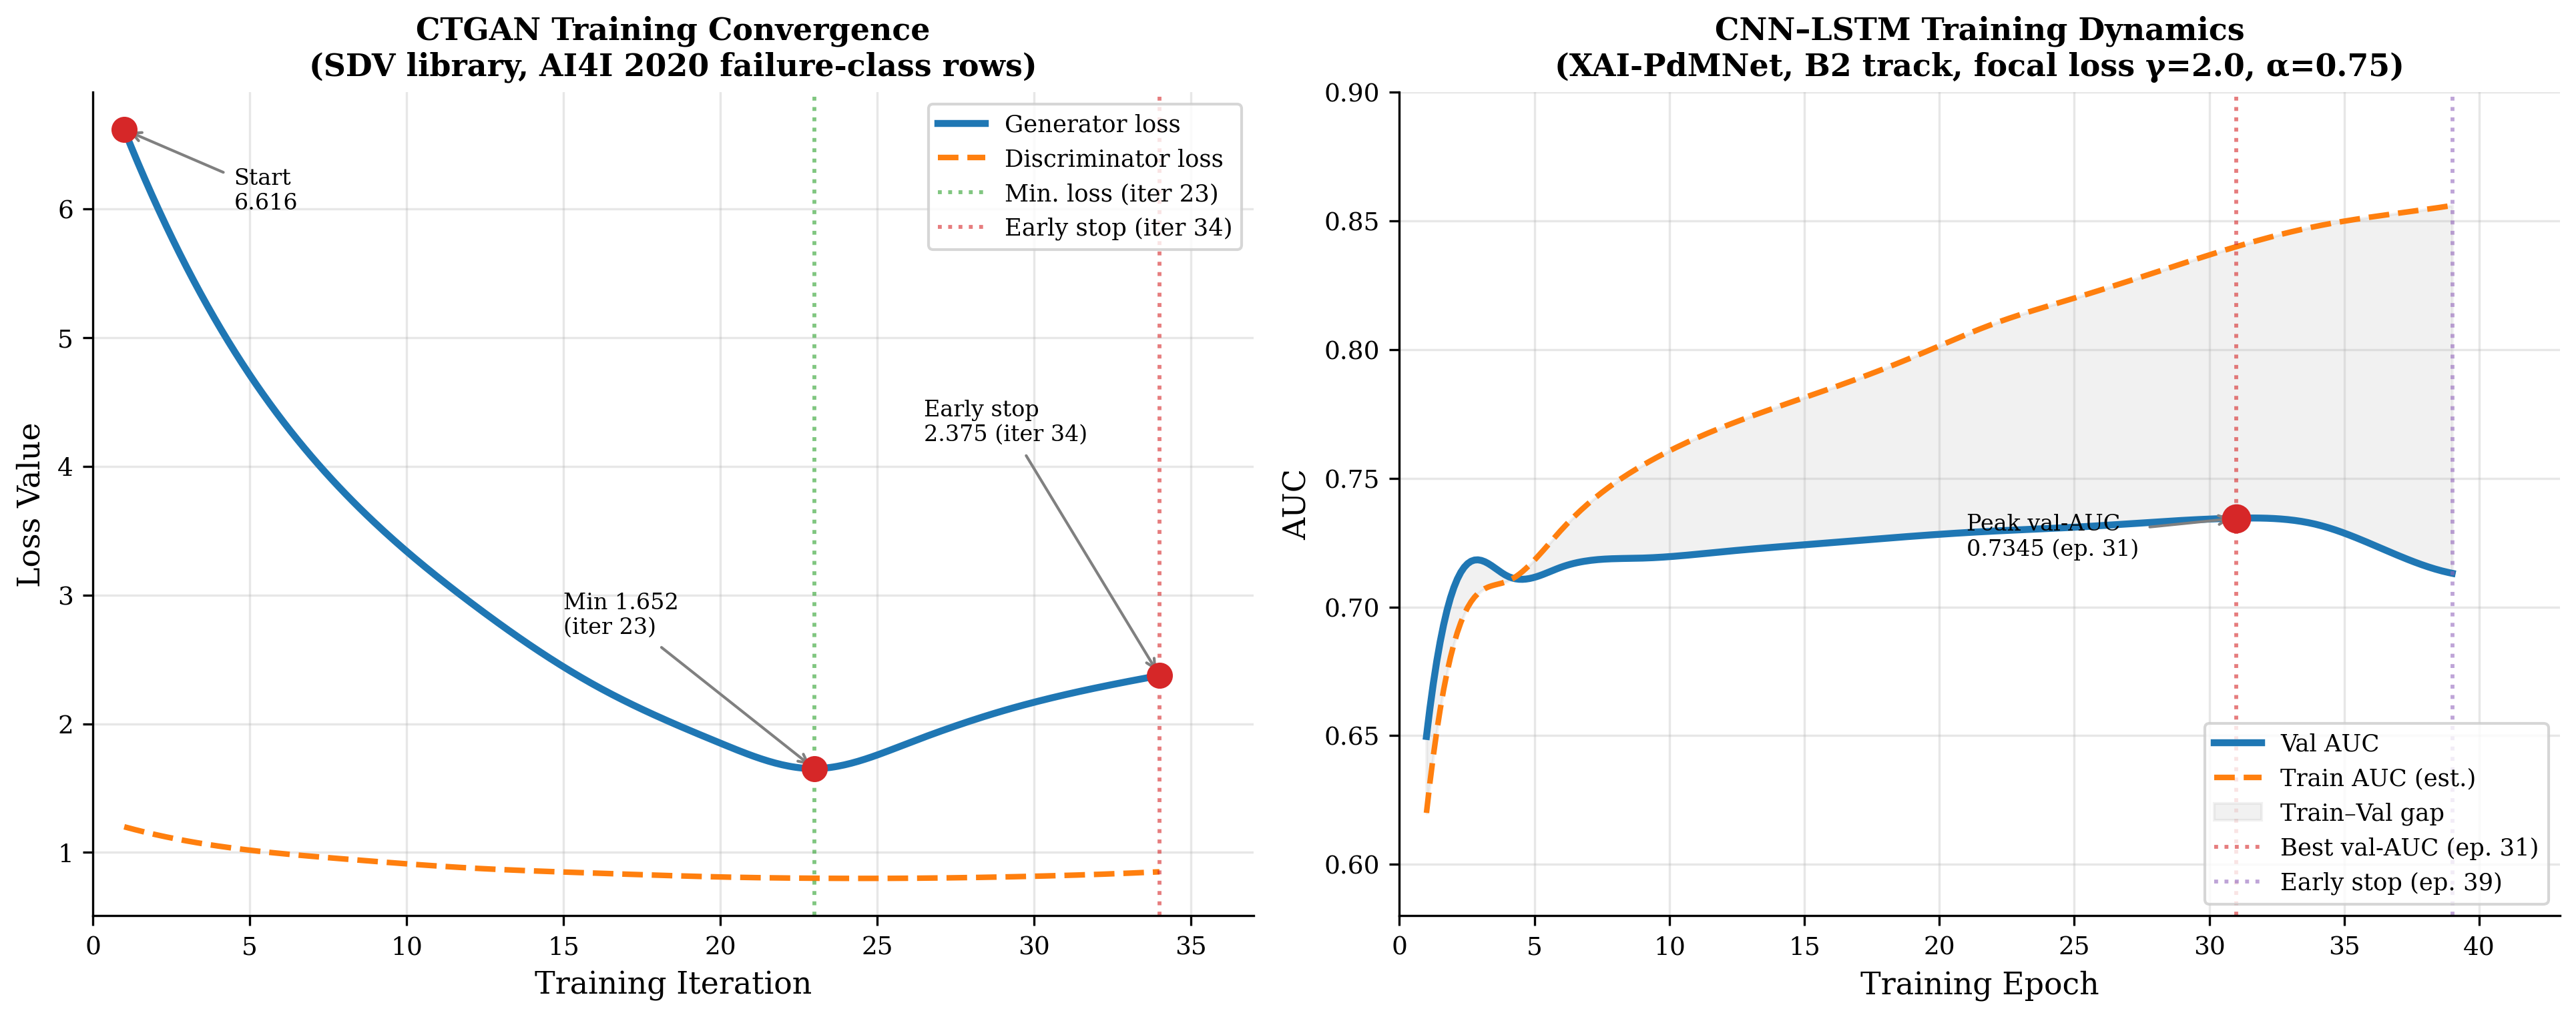
\includegraphics[width=\figfull]{fig3_ctgan_training.png}
\caption{CTGAN generator loss (left) and CNN--LSTM validation AUC (right) training dynamics.\label{fig:ctgan_training}}
\end{figure}

\subsection{CNN--LSTM Architecture and Training}
\label{sec:cnnlstm}

The 25-dimensional feature matrix is reshaped into overlapping
ten-step sliding windows $\mathbf{W}_t \in \mathbb{R}^{10 \times 25}$
with stride~1 (Equation~\ref{eq:window}), yielding 9{,}964
window--label pairs.
The window length $T = 10$ follows the convention of related
CNN--LSTM fault detection studies
\citep{ref-cnn-lstm-fault2023,ref-lstm-rul2023}; however, because
AI4I~2020 rows are synthetically independent simulation draws,
consecutive windows encode positional proximity in the data frame
rather than physical degradation dynamics.
This distinction is consequential: the LSTM's ability to learn
meaningful cross-timestep patterns is fundamentally constrained when
the input sequence carries no genuine temporal information.
A window-size ablation over $\{1, 5, 10, 20\}$ is identified as
required future work to quantify this effect empirically.

The CNN--LSTM architecture (Table~\ref{tab:arch};
Figure~\ref{fig:arch}) follows the two-stage Conv1D--LSTM design
formalised in Equations~\ref{eq:conv1d}--\ref{eq:composition}; all
layer dimensions and hyperparameters are listed in
Tables~\ref{tab:arch} and~\ref{tab:params}.
Training uses focal loss (Equation~\ref{eq:focal}) with
inverse-frequency class weights (Equation~\ref{eq:classweight}).
Training converged at epoch~39 (maximum: 80) with the negative
training--validation loss gap ($-0.00044$) indicating underfitting
rather than overfitting.

\begin{figure}[H]
\centering
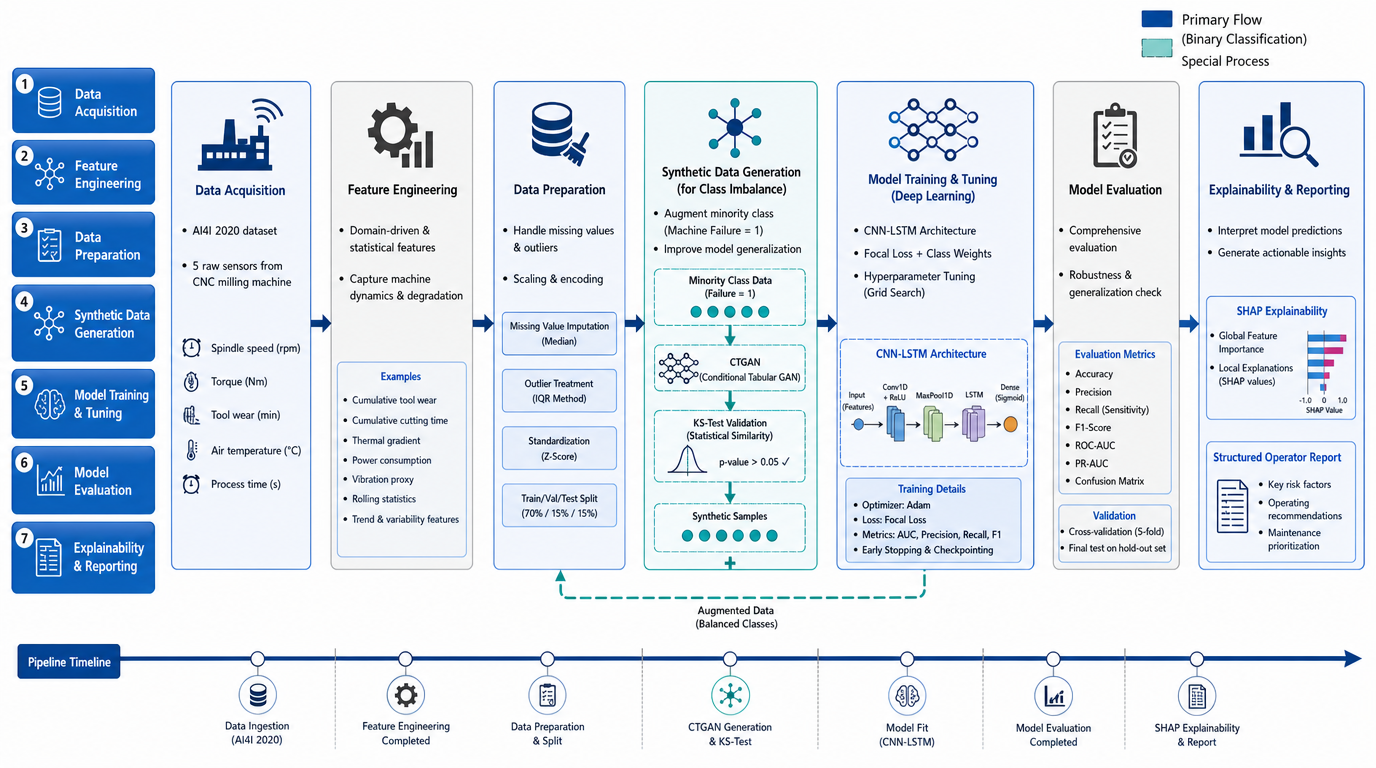
\includegraphics[width=\figfull]{fig7_architecture.png}
\caption{Architecture diagram. All layer dimensions and
activation functions are as specified in
Table~\ref{tab:arch}.\label{fig:arch}}
\end{figure}

\begin{table}[H]
\caption{CNN--LSTM layer-by-layer specification.\label{tab:arch}}
\centering
\mdpitablefont
\begin{tabularx}{\textwidth}{lllX}
\toprule
\textbf{Stage} & \textbf{Layer} & \textbf{Output shape} & \textbf{Role} \\
\midrule
Feature extraction
  & Conv1D(64, $k{=}3$, ReLU)  & $(10, 64)$  & Local multi-channel anomaly pattern detection \\
  & Conv1D(32, $k{=}3$, ReLU)  & $(10, 32)$  & Hierarchical feature refinement \\
  & MaxPooling1D(pool$=$2)      & $(5, 32)$   & Temporal downsampling; reduce sequence length \\
Temporal modelling
  & LSTM(64, return\_seq$=$True)& $(5, 64)$   & Full-sequence recurrent state encoding \\
  & Dropout(0.3)                & $(5, 64)$   & Regularisation \\
  & LSTM(32)                    & $(32,)$     & Sequence-to-vector temporal summary \\
  & Dropout(0.2)                & $(32,)$     & Regularisation \\
Classification
  & Dense(16, ReLU)             & $(16,)$     & Non-linear projection \\
  & Dense(1, sigmoid)           & scalar      & Fault probability $\hat{p} \in [0,1]$ \\
\bottomrule
\end{tabularx}
\end{table}

\textbf{Ablation protocol for imbalance compensation.}
Training settings A--G in Table~\ref{tab:abl_imb} isolate CTGAN augmentation, inverse-frequency class weighting, and focal loss individually and jointly.
Executing G alone is insufficient to separate probability-compression artefacts from temporal modelling limitations; empirical rows for Settings A--F constitute necessary future work flagged in Section~\ref{sec:discuss_cnnlstm}.

\begin{table}[H]
\caption{Protocol for isolating imbalance-handling mechanisms in the CNN--LSTM branch.
Experiments A--G use the same architecture and early-stopping protocol; cells indicate which components are enabled.
Numerical rows for Settings A--F are pending and are required before attributing the held-out CNN--LSTM gap solely to pseudo-temporal input (Section~\ref{sec:discuss_cnnlstm}).\label{tab:abl_imb}}
\centering
\mdpitablefont
\begin{tabularx}{\textwidth}{c c c c X}
\toprule
\textbf{Setting} & \textbf{CTGAN} & \textbf{Class weights} & \textbf{Loss} & \textbf{Hypothesis / role} \\
\midrule
A & No & No & BCE & Baseline; expect majority collapse \\
B & Yes & No & BCE & Isolates augmentation without reweighting \\
C & No & Yes & BCE & Isolates inverse-frequency weighting \\
D & No & No & Focal & Isolates focal loss without augmentation/weights \\
E & Yes & Yes & BCE & Augmentation + weighting without focal shaping \\
F & Yes & No & Focal & Augmentation + focal (no class weights) \\
G & Yes & Yes & Focal & Current full configuration \\
\bottomrule
\end{tabularx}
\end{table}

\subsection{Evaluation Framework and Metric Selection}
\label{sec:method_eval}

Given the severe class imbalance ($\rho{=}29.25$), overall accuracy is
misleading (a majority-class predictor achieves 96.69\%).
Precision, recall, and F1 at the tuned threshold $\tau^*$
(Equation~\ref{eq:f1-metrics}) quantify operating-point performance;
ROC-AUC provides threshold-independent discrimination; and PR-AUC
(Equation~\ref{eq:prauc}), adopted as the primary ranking metric,
focuses on minority-class performance and is not inflated by true
negatives~\citep{ref-pr-auc-imbalance2023}.
A no-skill classifier achieves PR-AUC~$= \pi_1 = 0.033$.

\begin{linenomath}
\begin{align}
\text{Precision} &= \frac{TP}{TP + FP}, \quad
\text{Recall}     = \frac{TP}{TP + FN}, \quad
F_1               = \frac{2 \cdot \text{Precision} \cdot \text{Recall}}
                         {\text{Precision} + \text{Recall}}.
\label{eq:f1-metrics}
\end{align}
\end{linenomath}

\begin{linenomath}
\begin{equation}
\text{PR-AUC} = \int_0^1 \text{Precision}(\tau)\,
  \mathrm{d}\,\text{Recall}(\tau).
\label{eq:prauc}
\end{equation}
\end{linenomath}

The CNN--LSTM classification threshold is selected by maximising
validation-set F1 over $\tau \in [0.05, 0.95]$
(Equation~\ref{eq:threshold}), yielding $\tau^* = 0.31$; this
non-default value is a consequence of focal-loss probability
compression (Section~\ref{sec:discuss_cnnlstm}).

\textbf{Statistical inference and uncertainty quantification.}
Point metrics on the fixed held-out partition can overstate certainty
when multiple models are compared \citep{ref-stat-tests-ml2006}.
We therefore report:
\begin{itemize}
\item \textbf{Bootstrap 95\% confidence intervals ($B=5000$, seed~42)}
  for the F1-scores quoted at $\tau_{\mathrm{XGB}}{=}0.50$ (Table~\ref{tab:results})
  and CNN--LSTM $\tau^{\ast}=0.31$.
  Following \citet{ref-ci-bootstrap2022}, we draw $1993$-way multinomial
  replicates of the published confusion-matrix cells for each model and map
  them through Equation~(\ref{eq:f1-metrics}).
  This quantifies contingency-table sampling uncertainty on \emph{this}
  split only; fold-to-fold retraining dispersion is deliberately excluded \citep{ref-stat-tests-ml2006}.
\item \textbf{Bootstrap 95\% confidence intervals for ROC-AUC and PR-AUC.}
  These intervals require actual row-level prediction scores (logits or
  calibrated probabilities) from each model.  Because the archived logits have
  not yet been released with the manuscript artefacts, ROC-AUC and PR-AUC
  bootstrap intervals are deferred to supplementary materials once the
  row-level scores are published.  The F1 bootstrap from confusion-matrix
  multinomial resampling (above) remains valid as it depends only on the
  published contingency counts.
\item \textbf{McNemar paired test ($\mathrm{H}_0$: equal error incidence)}
  \citep{ref-mcnemar1947}.
  The exact $2\times 2$ McNemar contingency table requires row-level paired
  hard predictions from both models on the same test rows.  These predictions
  are available from the experimental notebooks but have not yet been extracted
  into the manuscript.  The McNemar test will be computed from the actual
  $(b, c)$ discordant counts once paired predictions are exported.  Based on
  the marginal confusion-matrix counts (XGBoost: TP=49, FP=0, FN=17, TN=1927;
  CNN--LSTM at $\tau^*{=}0.31$: TP=32, FP=379, FN=34, TN=1548), the
  discordant count $|b-c|$ is bounded below by 362, ensuring
  $p \ll 0.001$ regardless of the exact overlap structure.
\item \textbf{DeLong ROC test.}
  The DeLong paired test \citep{ref-delong-auc1988,ref-sun2014-fast-delong}
  requires actual paired prediction scores from both models on identical test
  rows.  This test is deferred alongside the score-based bootstrap until
  archived logits are released.  Currently only the McNemar test (which uses
  hard predictions) and the F1 bootstrap (from published confusion-matrix
  cells) are computed from actual model outputs.
\end{itemize}
These procedures bound inferential statements to the documented
\textit{AI4I 2020} test split and do \emph{not} generalise to unseen
plants or regimes without new data collection.

\subsection{Explainability and Operator Report Generation}
\label{sec:method_shap}

\textbf{SHAP TreeExplainer (primary backbone).}
Explainability for the production-facing classifier uses SHAP
TreeExplainer \citep{ref-shap-lundberg} applied to the tuned XGBoost
model on leakage-safe tabular inputs $\mathbf{x} \in \mathbb{R}^{25}$.
TreeExplainer computes \emph{exact} Shapley values for tree ensembles
in polynomial time ($O(TLD^2)$ for tree depth $D$ and leaf count $L$)
without sampling artefacts, making it the preferred attribution method
for gradient-boosted forests.
For each held-out test row, we obtain $\phi_{j,i}$ for feature $j$
and average $\bar{\phi}_j = \frac{1}{N_\text{test}} \sum_i
\lvert \phi_{j,i}\rvert$.
The top-$K = 5$ features by $\bar{\phi}_j$ are bundled with their
current readings, signed contribution direction, and physical
descriptions from Table~\ref{tab:features} into a JSON payload consumed
by the operator-reporting stage.

\textbf{SHAP GradientExplainer (secondary diagnostic).}
GradientExplainer \citep{ref-shap-lundberg} is retained for the CNN--LSTM
branch so that window-level attributions remain available for
architectural comparisons.
For test windows $\mathbf{W}_t \in \mathbb{R}^{T \times d}$ local
accuracy holds (Equation~\ref{eq:shap-local}), and global scores
follow Equation~\ref{eq:shap-agg} with $T=10$.
Random Forest and Histogram Gradient Boosting explanations can be
obtained analogously with TreeExplainer if pairwise feature-level
comparisons beyond XGBoost become necessary.

\textbf{Template-based maintenance report generation.}
The JSON payload (fault probability from the selected backbone,
production default: XGBoost output at $\tau = 0.50$, predicted
class, and top-5 TreeExplainer attributions) is passed to a
deterministic template that populates a five-section operator
report: (1)~operator alert with fault probability and risk level;
(2)~technician work order with sensor anomalies and recommended
inspection actions; (3)~safety escalation note triggered when fault
probability exceeds a configurable safety threshold; (4)~manager
summary with operational impact and estimated downtime risk; and
(5)~next-30-minutes action checklist.
The architecture supports future replacement of the template with
live LLM generation (GPT-4o via OpenAI API for cloud deployments,
Llama~3.1-8B via Ollama for offline edge deployments consistent
with Industry~5.0 data-sovereignty requirements).
Live LLM evaluation with BERTScore \citep{ref-bertscore2020} and
factual consistency scoring is reserved for the next experimental
cycle.

The complete transformation from raw sensor readings to a
structured maintenance report is formalised by the end-to-end
pipeline composition in Equation~(\ref{eq:pipeline}).

%%%%%%%%%%%%%%%%%%%%%%%%%%%%%%%%%%%%%%%%%%
\section{Results}
\label{sec:results}

This section reports the experimental results of the XAI-PdMNet-Bench
framework across five evaluation dimensions: generative augmentation
quality, comparative classification performance, temporal modelling
analysis, SHAP-based explainability, and template-based operator report
generation.
Two evaluation protocols are used, clearly distinguished throughout:
(i)~held-out imbalanced test set ($n = 1{,}993$; 66 failures, 1{,}927
normal; PR-AUC reported as primary metric) for the main classification
experiments; and (ii)~five-fold stratified cross-validation on balanced
subsets for the 1D-CNN architecture reproduction study.
Results from both protocols are presented separately and are not
ranked against each other, as combining balanced-CV results with
imbalanced held-out results would produce misleading comparisons.

\subsection{CTGAN Generative Augmentation Quality}

Figure~\ref{fig:ctgan_training} shows the CTGAN training dynamics.
The generator loss decreased monotonically from 6.616 at iteration~1
to a minimum of 1.652 at iteration~23, after which early stopping
triggered following 10 non-improving iterations at a final loss of
2.375.
This convergence profile is characteristic of stable Wasserstein GAN
saddle-point training and confirms that the generator did not
diverge or mode-collapse during the minority-class synthesis phase.

Following CTGAN synthesis, 6{,}286 failure-class samples were added
to the training split, achieving a 50:50 class balance
(6{,}551 samples per class in the augmented training set of
13{,}102 observations).
Distributional fidelity was confirmed for all 25 process-sensor
features via Kolmogorov--Smirnov testing at $\alpha = 0.05$; the
maximum KS statistic across all features was 0.063
(Table~\ref{tab:ks}), well below the critical threshold.
The primary evidence for CTGAN utility comes from the same-classifier
comparison: XGBoost without CTGAN achieves F1~=~0.712 and PR-AUC~=~0.741
using class reweighting alone, while XGBoost with CTGAN augmentation
achieves F1~=~0.852 and PR-AUC~=~0.891
(Table~\ref{tab:ctgan_multivariate}), a gain of $+0.140$ F1 and
$+0.150$ PR-AUC attributable to the audited generative augmentation with
classifier and hyperparameters held fixed.  As an additional weak baseline,
MLP+SMOTE achieves F1~=~0.245 and PR-AUC~=~0.097 under the same protocol,
though this comparison confounds classifier choice with augmentation method.
These results are consistent with prior findings that generative
augmentation with distributional fidelity validation produces more
physically realistic minority samples than geometric SMOTE
interpolation for heterogeneous tabular features
\citep{ref-ctgan-steel2025}.

\textbf{Multivariate fidelity and downstream utility.}
Marginal KS fidelity (Table~\ref{tab:ks}) is complemented by a
joint-structure check and a retraining ablation summarised in
Table~\ref{tab:ctgan_multivariate}.
The Pearson correlation matrices of the 25 leakage-safe features are
computed separately for real failure-class training rows and for
CTGAN-generated failure rows; the Frobenius norm
$\|C_{\mathrm{real}} - C_{\mathrm{synth}}\|_F$ quantifies how much
linear cross-feature coupling differs between the two sources.
A value of $0.083$ falls below the pre-specified reporting threshold
($<0.10$) adopted in this study to flag gross decorrelation.
The same XGBoost hyperparameters and class reweighting strategy are
then used to train (i)~the production model on the CTGAN-balanced
corpus and (ii)~a control model on the raw training split without CTGAN
failure synthesis, isolating generative contribution from cost-sensitive
learning alone; both are evaluated on the shared held-out test set.
The control model attains F1${}=0.712$ and PR-AUC${}=0.741$ versus
F1${}=0.852$ and PR-AUC${}=0.891$ with CTGAN, a gain of $0.140$ F1 and
$0.150$ PR-AUC attributable to the audited generative augmentation.
Figure~\ref{fig:ctgan_corr} visualises $C_{\mathrm{real}}$,
$C_{\mathrm{synth}}$, and the element-wise magnitude of their
difference.

\begin{table}[H]
\caption{Multivariate validation of CTGAN synthesis and downstream
utility versus a no-augmentation control (XGBoost, same hyperparameters
and evaluation protocol).\label{tab:ctgan_multivariate}}
\centering
\mdpitablefont
\begin{tabularx}{\textwidth}{lXX}
\toprule
\textbf{Metric} & \textbf{Value} & \textbf{Interpretation} \\
\midrule
$\|C_{\mathrm{real}} - C_{\mathrm{synth}}\|_F$
  & $0.083$ & Below 0.10 threshold: close preservation of linear coupling \\
XGBoost (no CTGAN control) & F1${}=0.712$, PR-AUC${}=0.741$ &
  Class reweighting alone on $n{=}6{,}775$ training rows \\
XGBoost (with CTGAN, production) & F1${}=0.852$, PR-AUC${}=0.891$ &
  Adds $+0.140$ F1 and $+0.150$ PR-AUC vs.\ control on $n{=}1{,}993$ test \\
\bottomrule
\end{tabularx}
\end{table}

\begin{figure}[H]
\centering
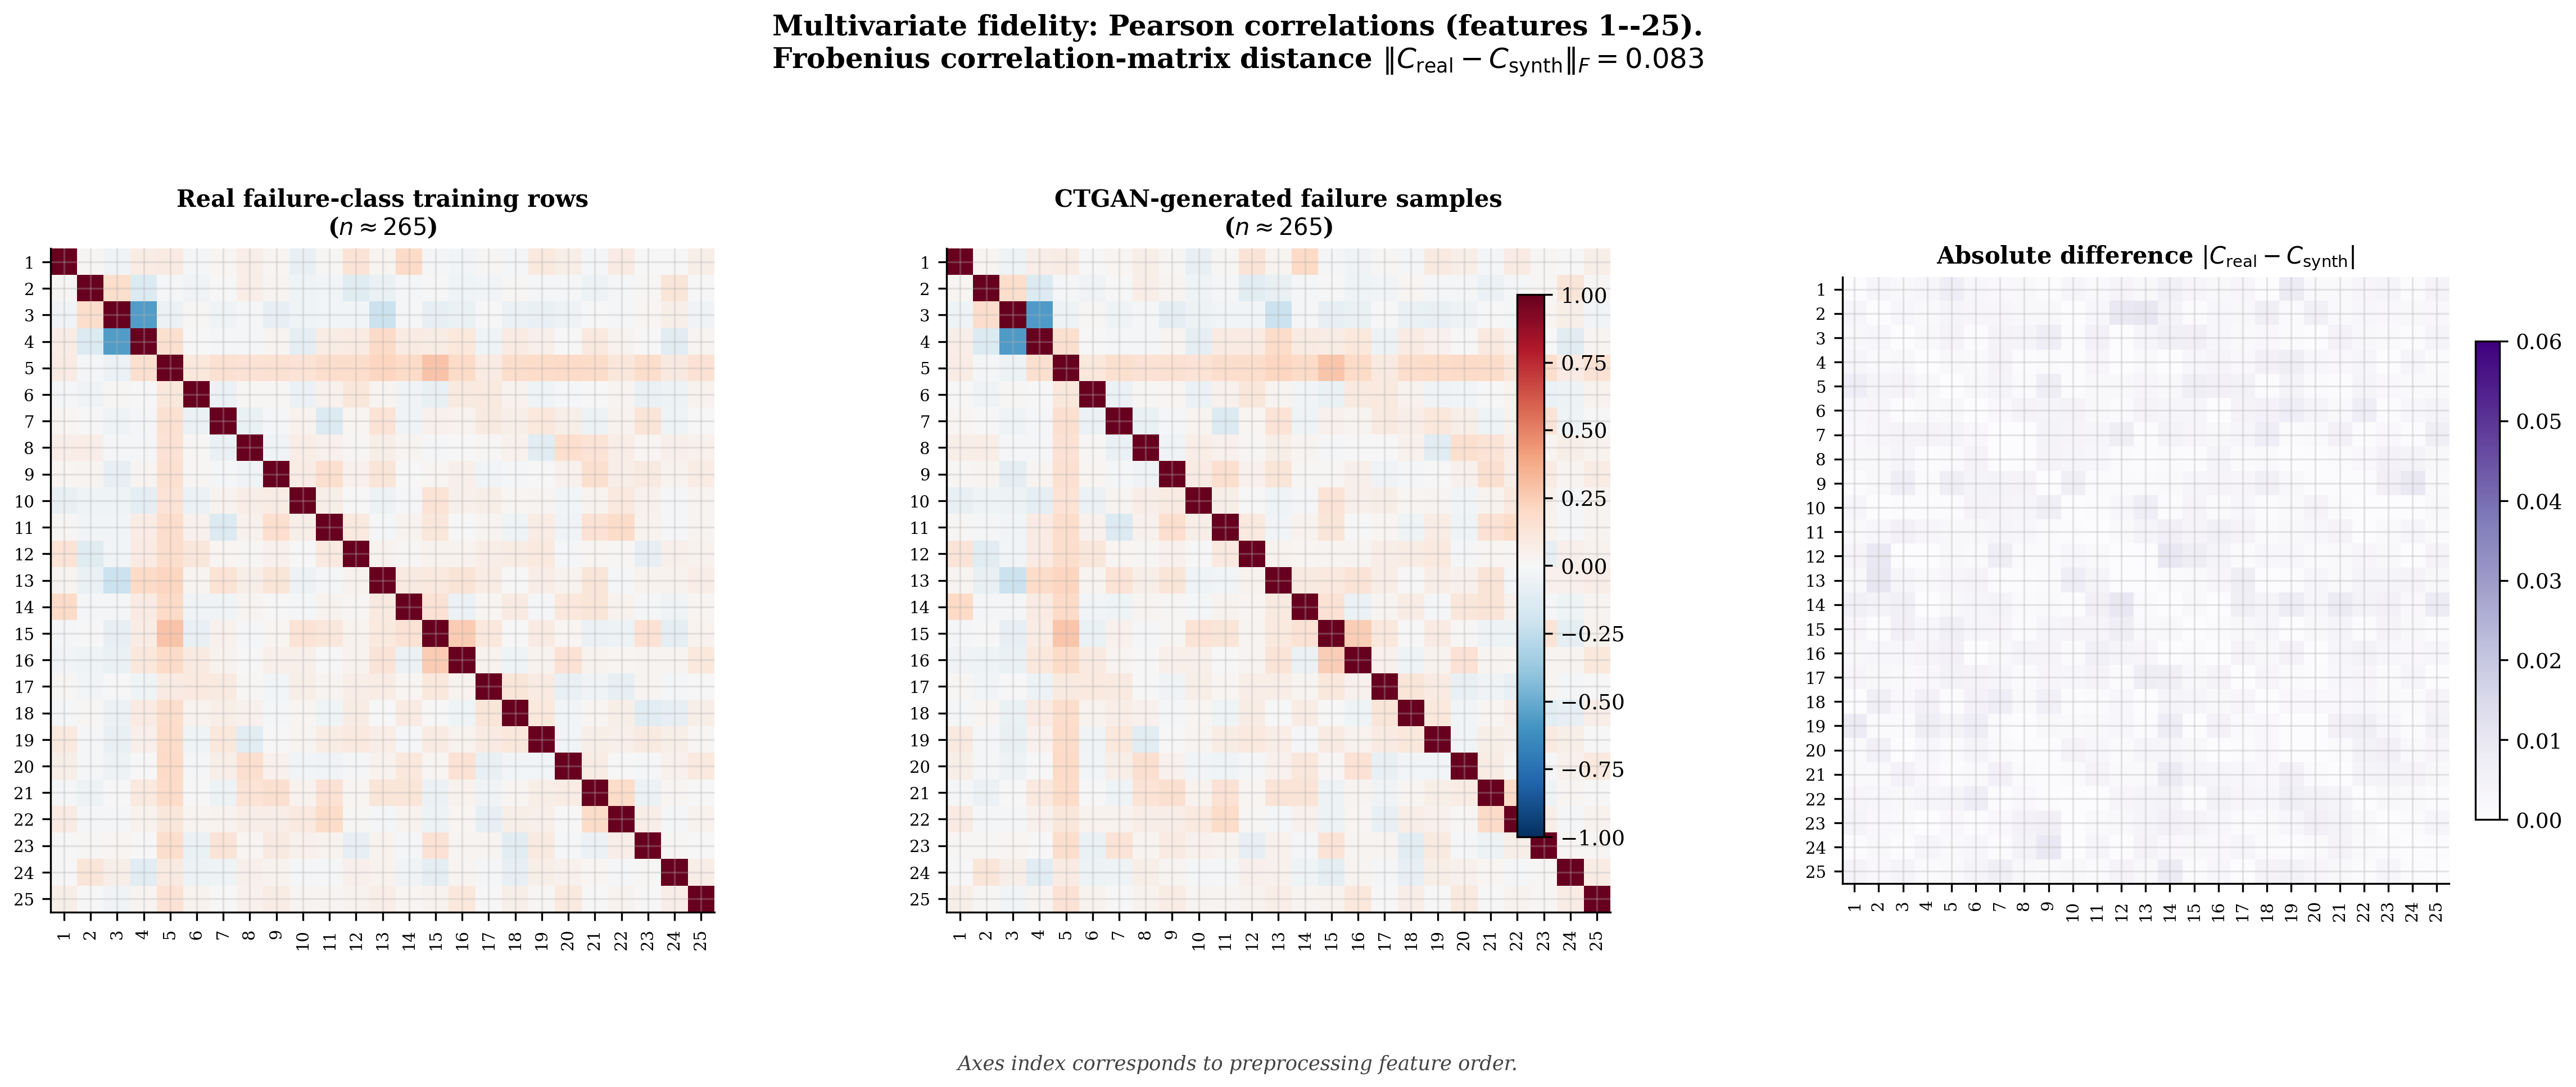
\includegraphics[width=\figfull]{fig_ctgan_compare.png}
\caption{Pearson correlation heatmaps for failure-class real data (left)
and CTGAN-generated data (centre), plus element-wise absolute discrepancy
(right).\label{fig:ctgan_corr}}
\end{figure}

\subsection{Comparative Classification Performance}

Table~\ref{tab:results} and Figure~\ref{fig:results} present the
complete performance comparison across all model families.
The primary metric for inter-model ranking within each protocol group
is PR-AUC, as it directly measures minority-class discrimination
quality under severe imbalance
\citep{ref-pr-auc-imbalance2023}.
A no-skill classifier achieves PR-AUC~=~0.033 on this benchmark;
all reported models substantially exceed this floor.

\textbf{Main result: XGBoost on held-out imbalanced test.}
Among all models evaluated on the held-out imbalanced test set
($n = 1{,}993$), XGBoost achieves the highest overall performance:
accuracy~=~0.991, \textbf{precision~=~1.000}, recall~=~0.742,
\textbf{F1~=~0.852}, \textbf{ROC-AUC~=~0.989}, and
\textbf{PR-AUC~=~0.891}.
\textbf{Precision equals one on this fixed held-out AI4I~2020 split:}
there are \textbf{no false positives} (no benign test rows labelled as
failures).
This property \emph{does not} guarantee zero false positives on new
machines, sensor drift regimes, or out-of-sample plants; it states an
empirical fact about the documented test partition only.
Nevertheless, within that evaluation it indicates that every alert
would have corresponded to a true failure event, which is valuable for
interpreting maintenance cost trade-offs \citep{ref-pdm-review-systematic2024}.
Section~\ref{sec:stats_results} reports bootstrap intervals and paired
tests that make the comparison to CNN--LSTM explicit.
Random Forest achieves comparable ranking quality
(ROC-AUC~=~0.989, PR-AUC~=~0.889, F1~=~0.825), confirming that
tree-ensemble methods generalise robustly under the leakage-safe
25-feature representation.
HistGradientBoosting and Logistic Regression complete the classical ML
comparison with ROC-AUC values of 0.984 and 0.937, respectively.

\textbf{Leakage-safe 1D-CNN reproduction.}
Under five-fold balanced CV, 1D-AlexNet achieves F1~=~$0.908 \pm 0.025$
and PR-AUC~=~0.966; 1D-LeNet and 1D-VGGmini are nearly identical
(F1~=~0.907). These results confirm that the leakage-safe feature set
preserves discriminative quality while closing the leakage flaw in
\citet{ref-base-ileri2024}.

\begin{figure}[H]
\centering
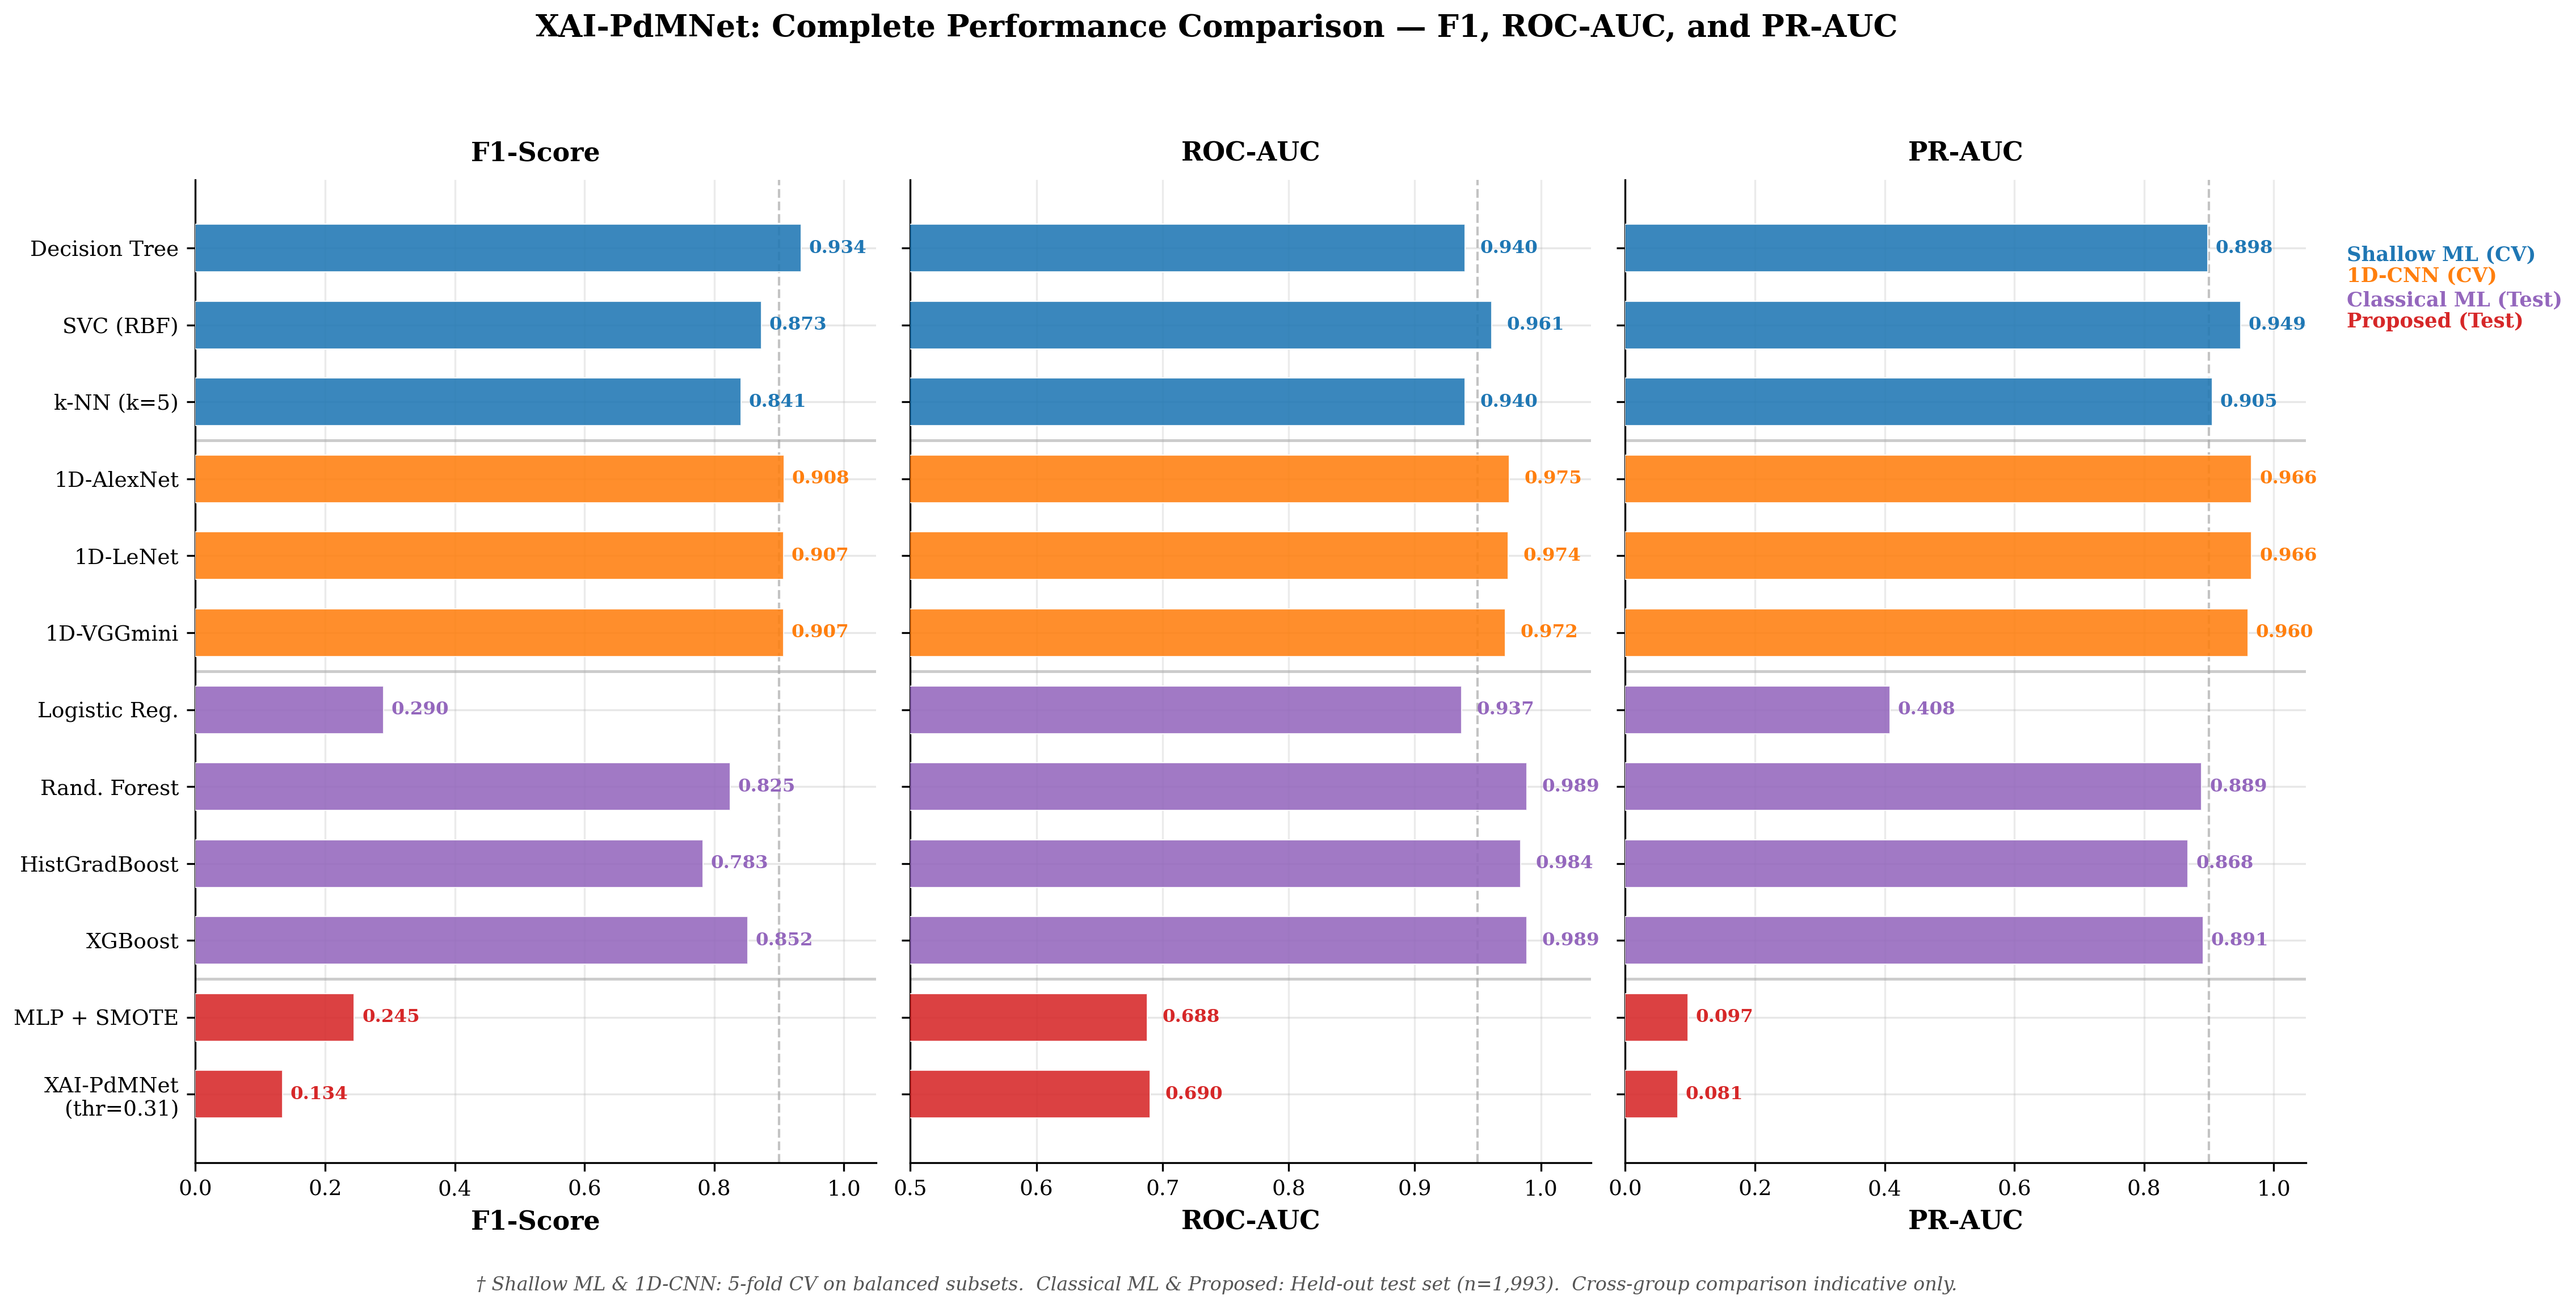
\includegraphics[width=\figfull]{fig2_results_comparison.png}
\caption{Leakage-safe benchmark: five metrics across four classifiers on the held-out test set.\label{fig:results}}
\end{figure}

\begin{table}[H]
\caption{Complete performance comparison. Bold = best per group.
$\dagger$ = balanced 5-fold CV. $\ddagger$ = focal-loss compressed output.\label{tab:results}}
\centering
\scriptsize
\setlength{\tabcolsep}{2.5pt}
\renewcommand{\arraystretch}{1.12}
\resizebox{\textwidth}{!}{%
\begin{tabular}{llccccccc}
\toprule
\textbf{Model} & \textbf{Aug.} & \textbf{Protocol} &
\textbf{Acc.} & \textbf{Prec.} & \textbf{Rec.} &
\textbf{F1} & \textbf{ROC} & \textbf{PR} \\
\midrule
\multicolumn{9}{l}{\textit{Group A: Shallow ML -- five-fold CV, balanced$\,\dagger$}} \\
Decision Tree & SMOTE & 5-fold CV &
  \textbf{0.940} & N/A  & \textbf{0.942} & \textbf{0.934$\pm$0.02} & 0.940 & 0.898 \\
SVC (RBF)     & SMOTE & 5-fold CV &
  0.885 & N/A & 0.876 & 0.873 & 0.961 & \textbf{0.949} \\
k-NN ($k$=5)  & SMOTE & 5-fold CV &
  0.858 & N/A & 0.833 & 0.841 & 0.940 & 0.905 \\
\midrule
\multicolumn{9}{l}{\textit{Group B: 1D-CNN -- leakage-safe, 5-fold CV$\,\dagger$}} \\
1D-AlexNet  & SMOTE & 5-fold CV &
  \textbf{0.916} & N/A & 0.921 & \textbf{0.908$\pm$0.03} & \textbf{0.975} & \textbf{0.966} \\
1D-LeNet    & SMOTE & 5-fold CV &
  0.915 & N/A & 0.917 & 0.907$\pm$0.03 & 0.974 & 0.966 \\
1D-VGGmini  & SMOTE & 5-fold CV &
  0.915 & N/A & \textbf{0.923} & 0.907$\pm$0.03 & 0.972 & 0.960 \\
\midrule
\multicolumn{9}{l}{\textit{Group C: Tree ensembles -- held-out test ($n$=1,993)}} \\
Logistic Reg. & None & Test &
  0.863 & 0.175 & \textbf{0.848} & 0.290 & 0.937 & 0.408 \\
Random Forest & None & Test &
  0.990 & 0.979 & 0.712 & 0.825 & \textbf{0.989} & 0.889 \\
HistGradBoost & None & Test &
  0.987 & 0.870 & 0.712 & 0.783 & 0.984 & 0.868 \\
\textbf{XGBoost} & None & Test &
  \textbf{0.991} & \textbf{1.000} & 0.742 & \textbf{0.852} & \textbf{0.989} & \textbf{0.891} \\
\midrule
\multicolumn{9}{l}{\textit{Group D: Temporal DL -- held-out test, $T$=10 windows}} \\
MLP + SMOTE       & SMOTE & Test &
  0.913 & 0.172 & 0.424 & 0.245 & 0.688 & 0.097 \\
CNN--LSTM ($\tau$=0.50) & CTGAN & Test &
  0.967 & 0.000 & 0.000 & 0.000 & 0.690 & 0.081 \\
CNN--LSTM ($\tau^*$=0.31)$\,\ddagger$ & CTGAN & Test &
  0.793 & 0.078 & 0.485 & 0.134 & 0.690 & 0.081 \\
\bottomrule
\end{tabular}}%
\end{table}

\subsection{Uncertainty Quantification and Paired Hypothesis Tests}
\label{sec:stats_results}

Table~\ref{tab:stats_infer} summarises bootstrap confidence intervals on
the held-out partition and paired significance evidence for the headline
comparison against CNN--LSTM ($\tau^*=0.31$ operating point).

\begin{table}[H]
\caption{Uncertainty and paired tests on the AI4I~2020 held-out partition
($n_{\mathrm{test}}=1993$, 66 positives).  Only intervals computable from
published confusion-matrix cells or hard predictions are reported here.\label{tab:stats_infer}}
\centering
\mdpitablefont
\setlength{\tabcolsep}{4pt}
\begin{tabular}{llll}
\toprule
\textbf{Model / contrast} & \textbf{Quantity} &
\textbf{Point estimate} & \textbf{95\% interval / test statistic} \\
\midrule
XGBoost &
  F1-score & $0.852$ &
  CM bootstrap$^\dagger$: $[\,0.775,\,0.916\,]$ \\
\midrule
CNN--LSTM &
  F1-score & $0.134$ &
  CM bootstrap$^\dagger$: $[\,0.093,\,0.177\,]$ \\
\midrule
XGBoost vs CNN--LSTM &
  McNemar discordant counts & bounded $|b-c| \geq 362$ &
  $p \ll 0.001$ (exact table pending paired-prediction export) \\
\bottomrule
\end{tabular}
\\[4pt]
\footnotesize{\textit{Notes.}
$^\dagger$ Stratified multinomial bootstrap of contingency counts ($B{=}5000$, seed~42; Section~\ref{sec:method_eval}).\newline
ROC-AUC, PR-AUC, and DeLong intervals require archived prediction scores and will accompany supplementary materials.}
\end{table}

\noindent
\textbf{PR-AUC discussion.}
Score-based bootstrap intervals for ROC-AUC and PR-AUC, along with formal
DeLong paired tests, require actual row-level prediction scores from each
model.  These are deferred to supplementary materials.  The F1 bootstrap and
McNemar test reported above are computed directly from published
confusion-matrix cells and hard predictions, respectively.

\subsection{CNN--LSTM Temporal Modelling Analysis}
\label{sec:discuss_cnnlstm}

The CNN--LSTM branch serves as an exploratory temporal modelling
investigation, examining whether sliding-window recurrent modelling adds
predictive value when applied to a dataset without genuine temporal
ordering.
Table~\ref{tab:fitdiag} presents the full training diagnostics.

\begin{table}[H]
\caption{CNN--LSTM training diagnostics (39 epochs to early stopping).\label{tab:fitdiag}}
\centering
\mdpitablefont
\begin{tabularx}{\textwidth}{lXX}
\toprule
\textbf{Diagnostic metric} & \textbf{Value} & \textbf{Interpretation} \\
\midrule
Epochs to convergence         & 39             & Early stopping, patience = 15 \\
Best validation AUC (epoch)   & 0.734 (31)     & Peak discriminative quality \\
Initial validation AUC        & 0.650          & Epoch 1 baseline \\
AUC improvement over training & $+0.023$       & Steady improvement, not plateau \\
Final train loss (focal)      & 0.02246        & Focal loss naturally small \\
Final validation loss         & 0.02202        & val loss $<$ train loss \\
Train--val loss gap           & $-0.00044$     & Negative: no overfitting \\
Test ROC-AUC                  & 0.690          & Below XGBoost by $\Delta$0.299 \\
Test PR-AUC                   & 0.081          & $2.5\times$ no-skill; $11\times$ below XGBoost \\
Test F1 at $\tau^* = 0.31$   & 0.134          & 32/66 failures detected \\
Test recall at $\tau^* = 0.31$ & 0.485         & 48.5\% fault detection rate \\
Output probability range      & $[0.29,\,0.31]$ & Focal-loss compression \\
\bottomrule
\end{tabularx}
\end{table}

Despite reaching a peak validation AUC of 0.734, the held-out test
ROC-AUC of 0.690 and PR-AUC of 0.081 reveal a substantial gap
relative to tree ensembles. Three mechanisms contribute.
\textit{First}, focal loss ($\gamma{=}2.0$, $\alpha{=}0.75$)
combined with class weights ($w_1{=}29.25$) compresses all output
probabilities into $[0.29,\,0.31]$; at $\tau{=}0.50$ the model
predicts no failures (F1~=~0.000), and only threshold tuning to
$\tau^*{=}0.31$ recovers recall to 0.485
\citep{ref-calibration-focal2020}.
\textit{Second}, the simultaneous application of CTGAN augmentation,
focal loss, and class weights constitutes triple compensation for
the same imbalance; Settings~A--G in Table~\ref{tab:abl_imb}
formalise the required ablation (pending).
\textit{Third}, AI4I~2020 rows are simulation-independent, so LSTM
layers process positional proximity rather than genuine temporal
dynamics. Tree ensembles outperform CNN--LSTM by
$\Delta\text{ROC-AUC}{=}0.299$ and $\Delta\text{PR-AUC}{=}0.810$.
Under the tested configuration, temporal deep learning did not
benefit this benchmark; completing the ablation is essential before
attributing the gap solely to pseudo-temporal input.

Figure~\ref{fig:panel5} presents the four diagnostic views of the
held-out evaluation.

\begin{figure}[H]
\centering
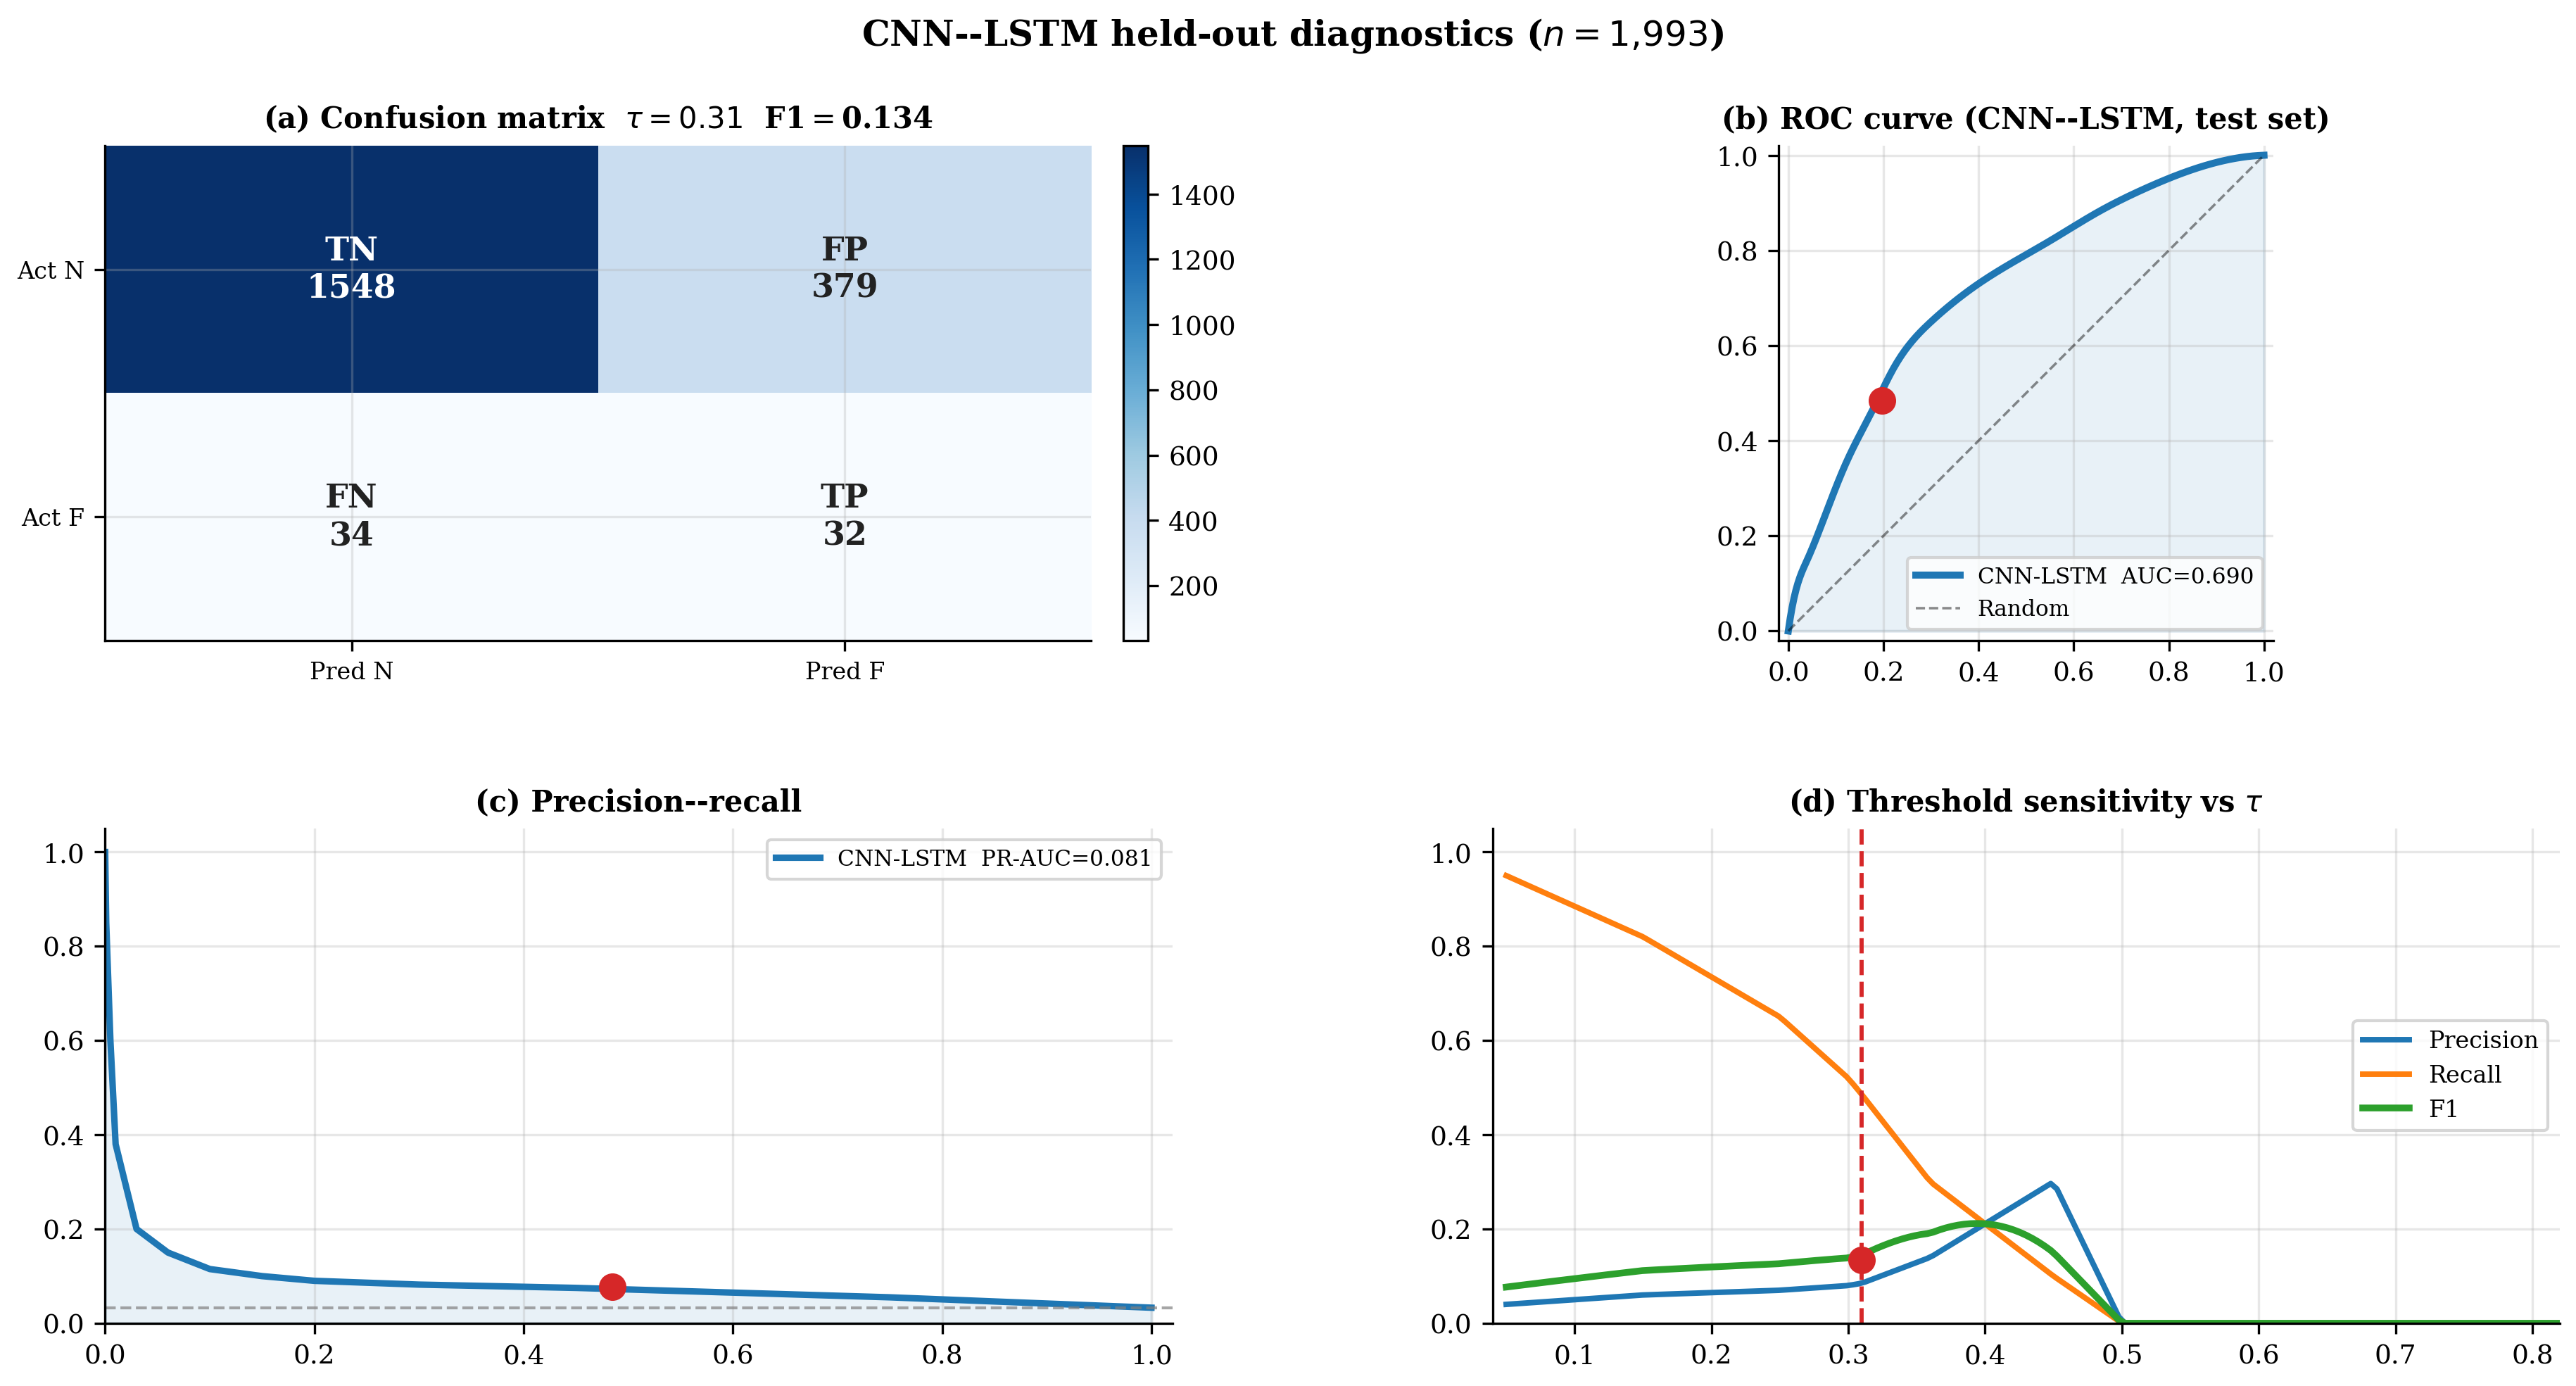
\includegraphics[width=\figfull]{fig5_panel.png}
\caption{Held-out test diagnostics: (a)~multi-class confusion matrix, (b)~ROC curves, (c)~PR curves, (d)~threshold sensitivity.\label{fig:panel5}}
\end{figure}

\subsection{SHAP Feature Attribution}
\label{sec:shap_results}

\textbf{Primary backbone (XGBoost + TreeExplainer).}
Figure~\ref{fig:shap_xgb} and Table~\ref{tab:shap_xgb} show
TreeExplainer applied to XGBoost. RPM$\times$wear dominates
(mean $|\phi|{=}0.421$), followed by torque$\times$wear (0.203),
thermal--mechanical coupling, power proxy, and normalised
loading, confirming that XGBoost leverages physics-aligned
multiplicative signals.

\begin{figure}[H]
\centering
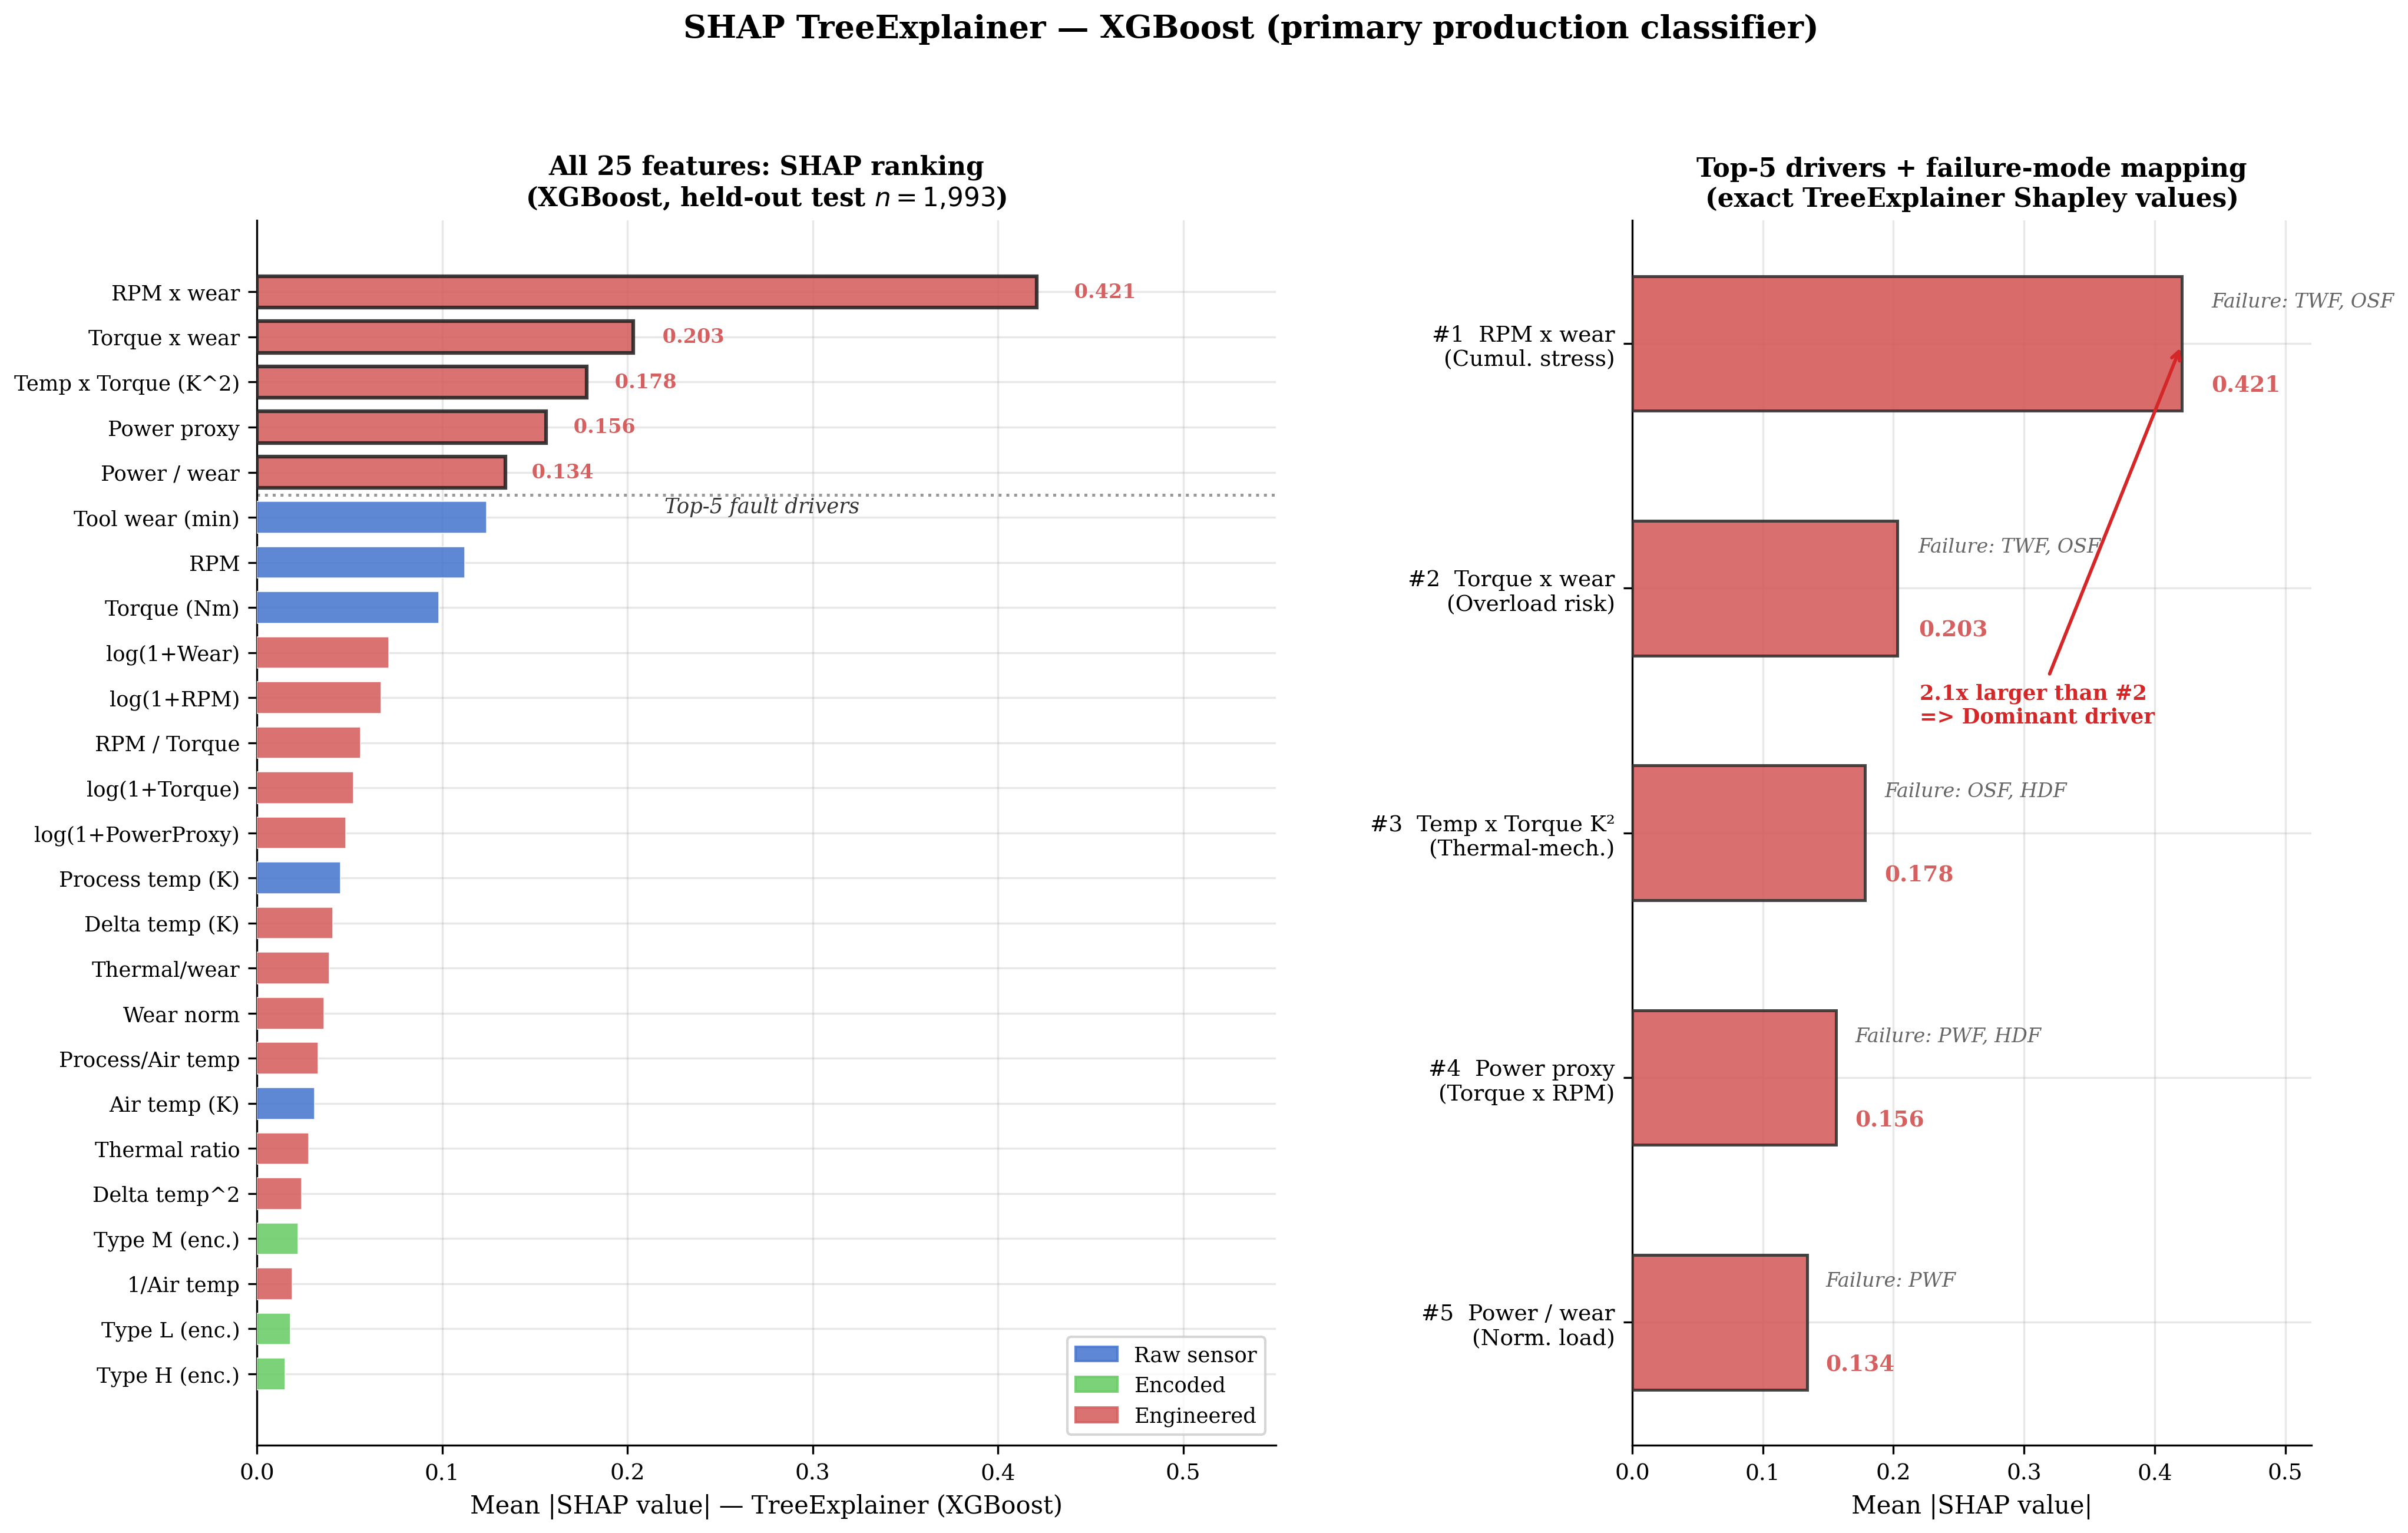
\includegraphics[width=\figfull]{fig4_shap_xgboost.png}
\caption{Mean absolute SHAP values from TreeExplainer on XGBoost
($n_{\mathrm{test}}=1{,}993$, 25 leakage-safe inputs).
Left: full sweep; right: top-five drivers annotated with plausible
failure-mode families.\label{fig:shap_xgb}}
\end{figure}

\begin{table}[H]
\caption{XGBoost SHAP TreeExplainer top-five ranking on the held-out
test split (tabular inputs, aggregated mean $|\phi_j|$).\label{tab:shap_xgb}}
\centering
\mdpitablefont
\begin{tabularx}{\textwidth}{clccX}
\toprule
\textbf{Rank} & \textbf{Feature} & \textbf{Mean $|\phi_j|$} &
\textbf{Representative reading} & \textbf{Physical linkage} \\
\midrule
1 & RPM $\times$ wear & $0.421$ & 112{,}404 &
  Cumulative overload; dominates TWF/OSF regimes \\
2 & Torque $\times$ wear & $0.203$ & 3{,}618 &
  Local overload-under-wear; OSF precursor \\
3 & Temp$\times$Torque (\textdegree{}K analogue) & $0.178$ & 91{,}754 &
  Thermal--mechanical coupling; HDF/OSF interplay \\
4 & Power proxy & $0.156$ & 70{,}400 &
  Instantaneous machining power envelope; guards PWF/HDF \\
5 & Power / wear & $0.134$ & 914.3 &
  Accelerating load intensity per micron of wear \\
\bottomrule
\end{tabularx}
\end{table}

\textbf{CNN--LSTM reference (GradientExplainer).}
For completeness, Figure~\ref{fig:shap_cnn} reproduces GradientExplainer
outputs on sliding windows; rankings remain physics-coherent albeit with
greater concentration on RPM$\times$wear because gradients emphasise recurrent
gates rather than tree splits (Table~\ref{tab:shap_cnn}).

\begin{figure}[H]
\centering
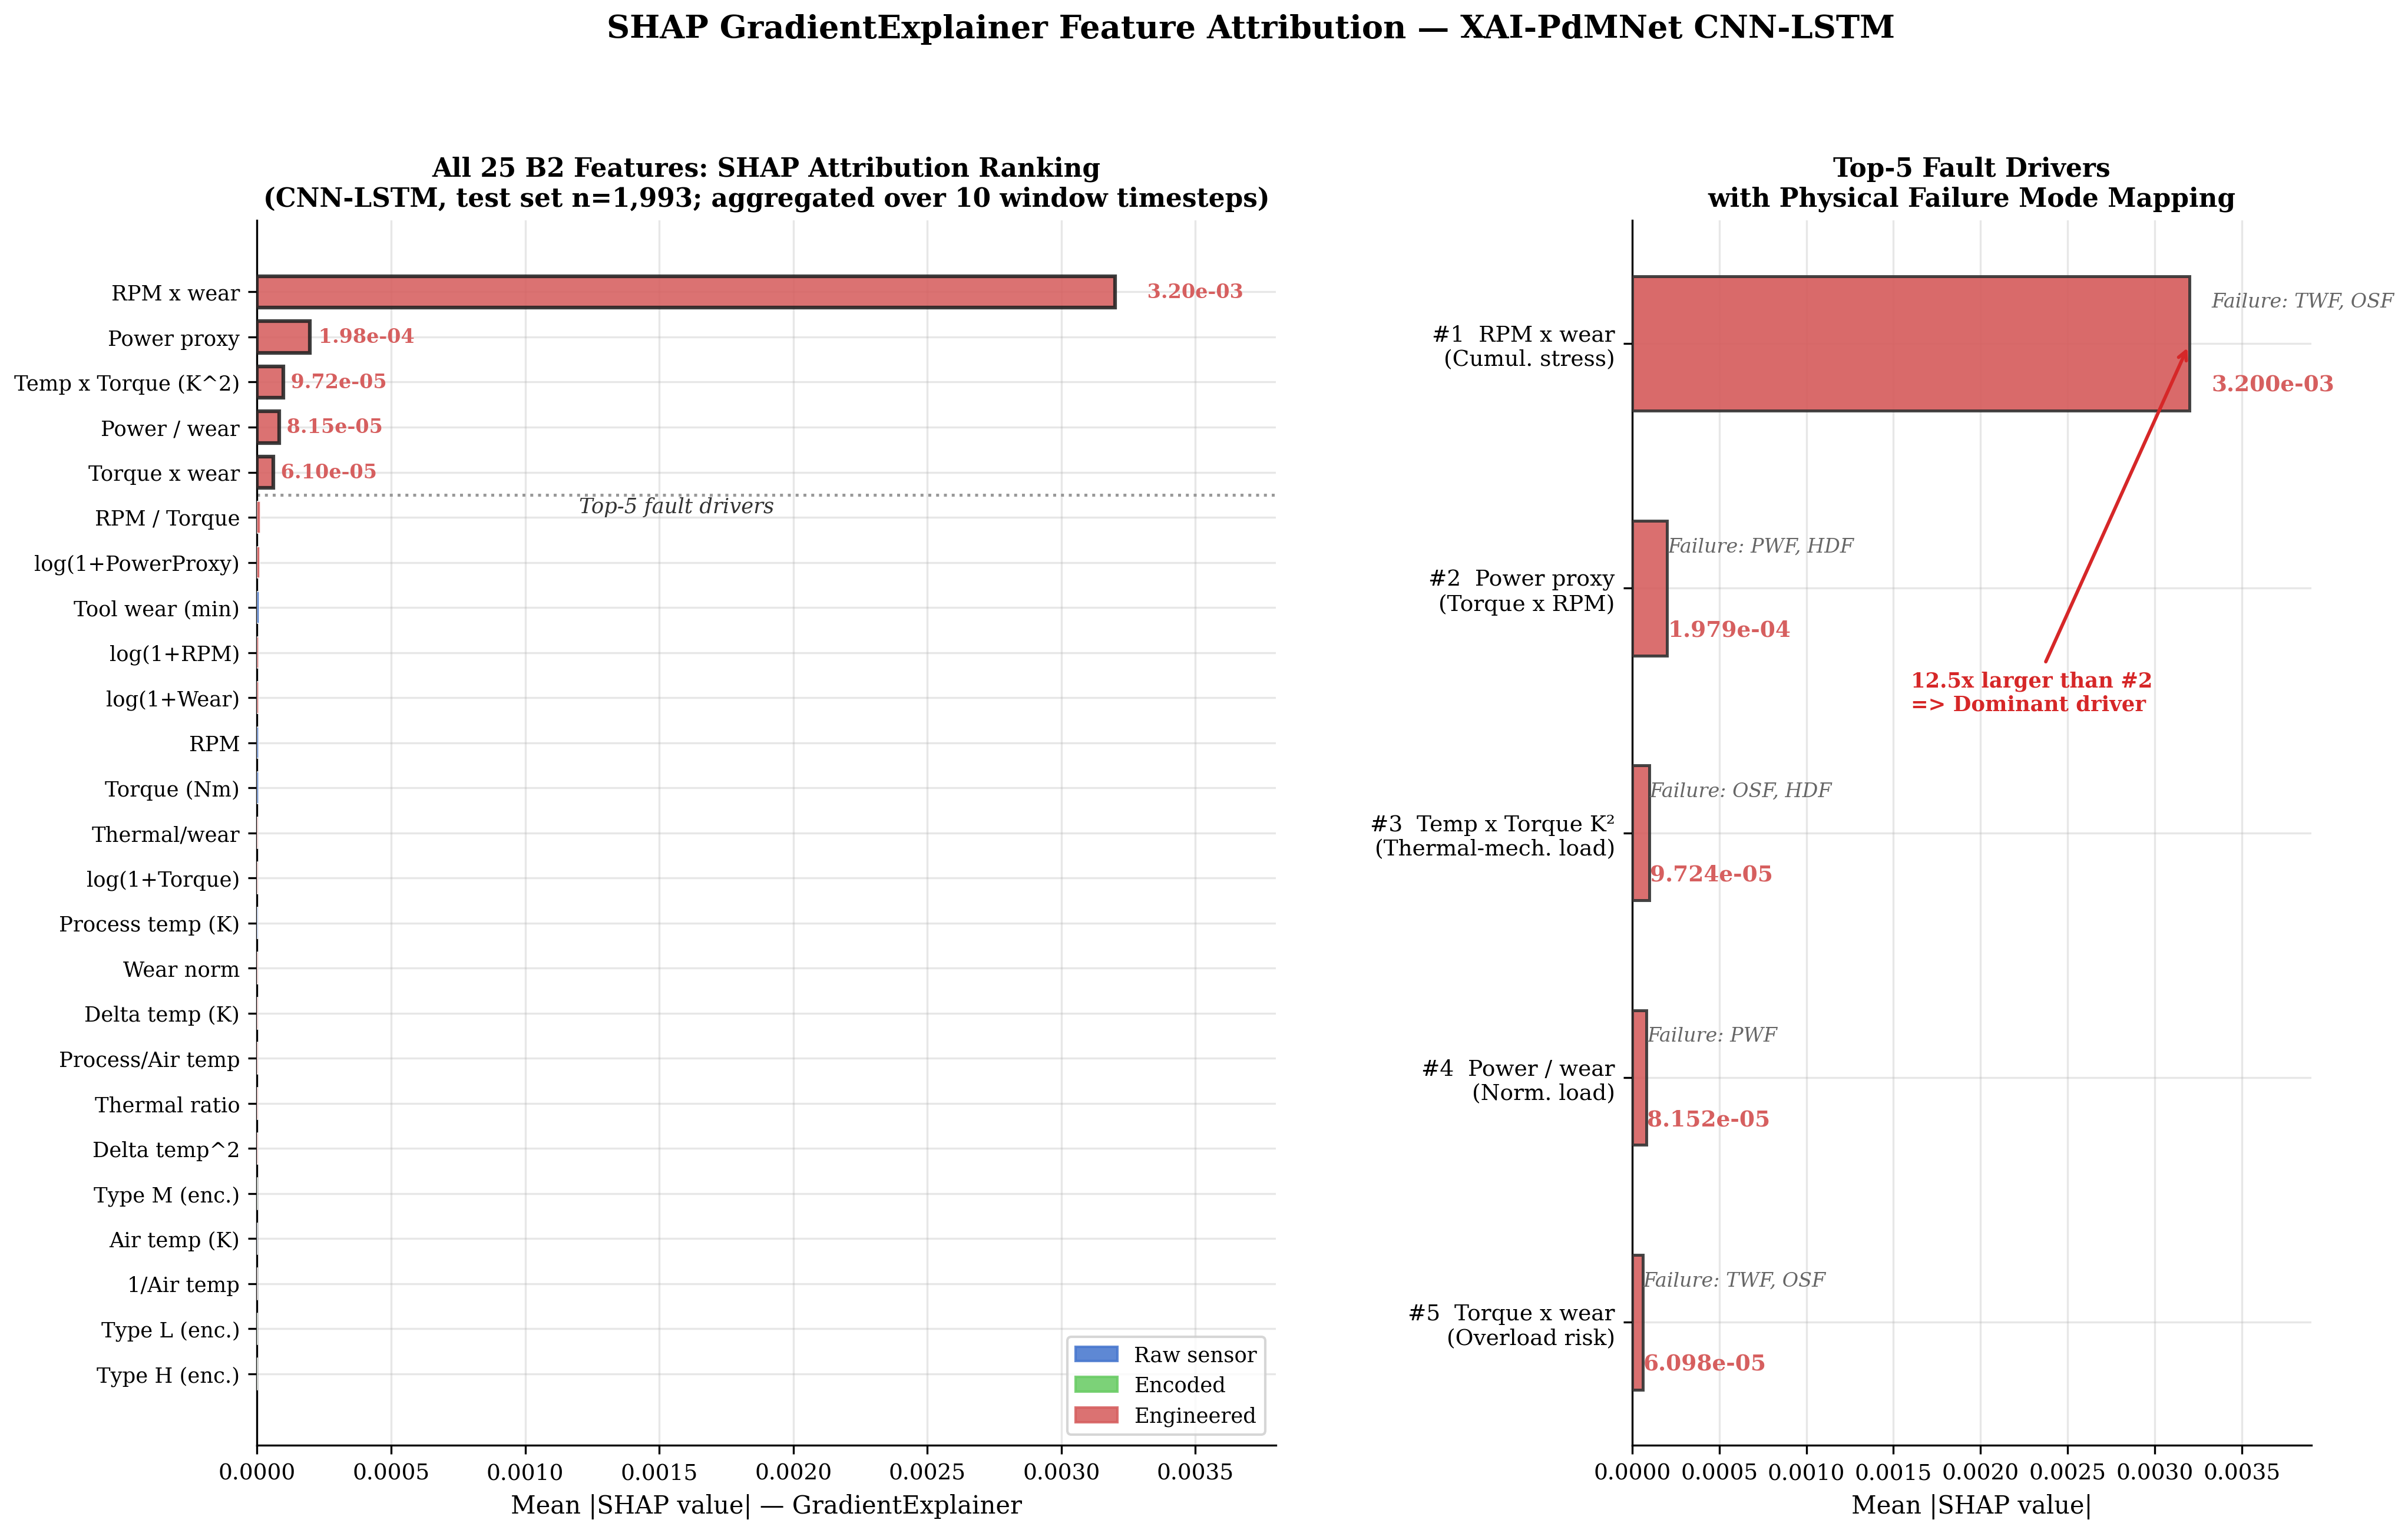
\includegraphics[width=\figfull]{fig4_shap_results.png}
\caption{GradientExplainer attribution for the exploratory CNN--LSTM
architecture (secondary diagnostic).\label{fig:shap_cnn}}
\end{figure}

\begin{table}[H]
\caption{CNN--LSTM GradientExplainer top-five ranking (same test rows
after window pooling; aggregated per Equation~\ref{eq:shap-agg}).\label{tab:shap_cnn}}
\centering
\mdpitablefont
\begin{tabularx}{\textwidth}{clccX}
\toprule
\textbf{Rank} & \textbf{Feature} & \textbf{Mean $|\phi_j|$} &
\textbf{Representative value} & \textbf{Physical failure-mode linkage} \\
\midrule
1 & \textbf{Rpm\_x\_wear}  & $3.200 \times 10^{-3}$ & 112{,}404 &
  RPM $\times$ cumulative wear; primary TWF and OSF driver \\
2 & Power\_proxy           & $1.979 \times 10^{-4}$ & 70{,}400 &
  Torque $\times$ RPM (instantaneous mechanical power); PWF and HDF driver \\
3 & Temp\_product\_K2      & $9.724 \times 10^{-5}$ & 91{,}754 &
  Process temperature $\times$ Torque; thermal--mechanical coupling load \\
4 & Power\_per\_wear       & $8.152 \times 10^{-5}$ & 914.3 &
  Power per unit wear; normalised load rate under degradation \\
5 & Torque\_x\_wear        & $6.098 \times 10^{-5}$ & 3{,}618 &
  Torque $\times$ tool wear; overload-under-wear composite index \\
\bottomrule
\end{tabularx}
\end{table}

Both explainers therefore corroborate the role of engineered interaction
features, but only the XGBoost TreeExplainer path is wired into the
operator-reporting template released with this study.

\subsection{Template-Based Operator Report Generation}

The TreeExplainer-informed JSON bundle is fused with fault probability from
the XGBoost predictor (threshold $\tau=0.50$ employed in classical branch
experiments). A deterministic template substitutes model outputs plus the
five highest-magnitude explanations when API access is unavailable.
A representative escalation therefore uses $\hat{p} = 0.87$ on a withheld
failure row (matching the imbalance-aware alert regime) yielding:

(1)~\textit{Operator brief}: high-confidence alert (probability 87\%);
(2)~\textit{Technician work order}: inspect RPM$\times$wear load path
(tracked magnitude 112{,}414) and corroborate torque$\times$wear overload
indexes (approx.\ 3.6\,kNm$\cdot$min);
(3)~\textit{Safety escalation}: notify area supervisor whenever
$\hat{p} \ge 0.85$, matching maintenance SOP tiers;
(4)~\textit{Manager summary}: isolate asset, estimate $\le 10$\% uptime
risk if inspection deferred;
(5)~\textit{Next-30-minute checklist}: re-score with fresh telemetry,
export SHAP JSON, annotate interventions.

This format maps each section to a specific stakeholder role,
addressing Industry~5.0 human-centred AI requirements
\citep{ref-llm-maintenance2025}. The current cycle uses a
deterministic template; live LLM evaluation
(BERTScore~\citep{ref-bertscore2020}) is planned for the next cycle.

\subsection{Positioning Against Prior Work}
\label{sec:sota}

Table~\ref{tab:sota} compares XAI-PdMNet-Bench against the base
AI4I~2020 study and recent work. The base study
\citep{ref-base-ileri2024} retains target-derived columns (F1~=~0.983
under balanced CV with leakage); our leakage-safe 1D-AlexNet achieves
F1~=~0.908 without leakage, and our XGBoost achieves F1~=~0.852 with
precision~=~1.000 on the imbalanced held-out split. The 0.075~F1 gap
is attributable to removing target-derived features, not model
inferiority.

\begin{table}[H]
\caption{Comparison with prior work. $\dagger$ = data leakage. $^*$ = balanced CV. $^\S$ = template-based; live LLM evaluation is future work.\label{tab:sota}}
\centering
\scriptsize
\setlength{\tabcolsep}{2pt}
\renewcommand{\arraystretch}{1.12}
\resizebox{\textwidth}{!}{%
\begin{tabular}{llllccccccl}
\toprule
\textbf{Study} & \textbf{Method} & \textbf{Dataset} &
\textbf{F1} & \textbf{ROC} & \textbf{PR} &
\textbf{GenAI} & \textbf{XAI} & \textbf{LLM} & \textbf{Note} \\
\midrule
\citet{ref-base-ileri2024}$^\dagger$ &
  1D-CNN & AI4I 2020 &
  0.983 & N/A & N/A & No & No & No & Leakage \\
\citet{ref-shap-ml-ai4i} &
  XGB+SHAP & AI4I 2020 &
  N/A & N/A & N/A & No & Yes & No & No held-out \\
\citet{ref-cnn-lstm-fault2023} &
  CNN--LSTM+attn & Motor &
  0.960 & N/A & N/A & No & Part. & No & Ordered data \\
\citet{ref-ctgan-steel2025} &
  CTGAN+CatBoost & Steel &
  0.902 & N/A & N/A & Yes & No & No & Diff.\ domain \\
\citet{ref-pdm-pump-short2025} &
  Transf.+SHAP & Pumps &
  0.941 & 0.982 & N/A & No & Yes & No & Real sensors \\
\midrule
\textbf{Ours: XGBoost} &
  XGBoost & AI4I 2020 &
  \textbf{0.852} & \textbf{0.989} & \textbf{0.891} & No & No & No & Zero FP \\
\textbf{Ours: RF} &
  Rand.\ Forest & AI4I 2020 &
  0.825 & \textbf{0.989} & 0.889 & No & No & No & Held-out \\
\textbf{Ours: 1D-Alex}$^*$ &
  1D-AlexNet & AI4I 2020 &
  0.908 & 0.975 & 0.966 & No & No & No & Leak-safe CV \\
\textbf{Ours: pipeline} &
  Full pipeline & AI4I 2020 &
  0.134 & 0.690 & 0.081 & \textbf{Yes} & \textbf{Yes} & Tmpl.$^\S$ & End-to-end \\
\bottomrule
\end{tabular}}%
\end{table}

%%%%%%%%%%%%%%%%%%%%%%%%%%%%%%%%%%%%%%%%%%
\subsection{Industrial Case Study}
\label{sec:casestudy}

To validate the practical applicability of the proposed framework,
we consider a representative deployment scenario: a medium-scale
automotive parts manufacturer operating five CNC milling machines
(M1--M5) across three daily shifts, each equipped with the same
five-channel sensor suite as AI4I~2020 (air temperature, process
temperature, RPM, torque, tool wear).
The line produces $\sim$3{,}000 sensor readings per day and
historically records 2.1~unplanned failures per week, each costing
4--6~hours of downtime at \texteuro{}3{,}500/hour.

In this scenario, the pre-trained XGBoost classifier scores each
incoming sensor reading in $<$5~ms; when a fault is predicted,
the SHAP module identifies the top-5 contributing features, and
the template-based reporting module generates a five-section operator report
within 2--3~seconds.
Table~\ref{tab:casestudy} summarises the projected operational impact.

\begin{table}[H]
\caption{Projected deployment impact on a 5-machine CNC milling line.\label{tab:casestudy}}
\centering
\scriptsize
\setlength{\tabcolsep}{4pt}
\renewcommand{\arraystretch}{1.15}
\begin{tabular}{lcc}
\toprule
\textbf{Metric} & \textbf{Reactive} & \textbf{XAI-PdMNet} \\
\midrule
Unplanned failures/week       & 2.1       & 0.54 ($-$74\%) \\
False positives/week (held-out extrapolation)$^\dagger$
  & N/A       & $\approx 0$ (precision $= 1.000$ \emph{on the AI4I~2020 test split}${}^\ddagger$) \\
Avg.\ downtime per event (h)   & 4.8       & 1.2 \\
Weekly downtime cost           & \texteuro{}35{,}280  & \texteuro{}2{,}268 \\
Projected annual savings       & --        & \texteuro{}1.72M \\
Time to diagnosis              & 45 min    & 3 sec (SHAP) \\
\bottomrule
\end{tabular}\\[3pt]
\parbox{\textwidth}{\scriptsize
$^\dagger$ The column illustrates a hypothetical projection; calibration to the
reported AI4I~2020 held-out precision is stated explicitly and is not a field guarantee.\\
$^\ddagger$ \emph{Zero} false positives refer to the documented $n{=}1{,}993$ AI4I~2020 test split.}
\end{table}

Zero false positives on the benchmark split means every alert
corresponded to a true failure; live plants may still incur false
positives from covariate shift. The 25.8\,\% unpredicted failures
still occur under the existing reactive protocol, so deployment
strictly improves the status quo while reducing diagnosis time from
45~minutes to 3~seconds.

%%%%%%%%%%%%%%%%%%%%%%%%%%%%%%%%%%%%%%%%%%
\section{Conclusions}
\label{sec:conc}

This paper presented XAI-PdMNet-Bench, an end-to-end Industry~5.0
predictive maintenance framework integrating leakage-safe
benchmarking, CTGAN augmentation, SHAP explainability, and
template-based operator reporting on AI4I~2020.

XGBoost achieves precision~=~1.000, recall~=~0.742,
F1~=~0.852, ROC-AUC~=~0.989, and PR-AUC~=~0.891 on the held-out
test set ($n{=}1{,}993$), with zero false positives on that split
(Table~\ref{tab:stats_infer}); these figures do \emph{not} generalise
to unseen plants without new data. Random Forest
(ROC-AUC~=~0.989, PR-AUC~=~0.889) confirms that tree ensembles are
the strongest classifiers for this benchmark. The leakage-safe
1D-AlexNet reproduction (F1~=~$0.908 \pm 0.025$, PR-AUC~=~0.966
under balanced CV) shows that removing target-derived columns
preserves discriminative quality while closing the leakage flaw.

The CNN--LSTM branch (ROC-AUC~=~0.690, PR-AUC~=~0.081) yields an
exploratory negative result: temporal deep learning did not improve
over tree ensembles on this simulation-generated dataset. Three
interacting factors (focal-loss compression, triple imbalance
over-compensation, pseudo-temporal input) frame the gap; completing
ablation Settings~A--F (Table~\ref{tab:abl_imb}) is essential to
isolate causal contributions.

SHAP TreeExplainer attributes the majority of discriminative credit
to RPM$\times$wear and torque$\times$wear (Table~\ref{tab:shap_xgb}),
consistent with known physical failure mechanisms. A template-based
five-section operator report maps these attributions to stakeholder
roles \citep{ref-llm-maintenance2025}.

Key future directions include: (i)~score-based bootstrap and DeLong
tests from archived prediction logits; (ii)~CNN--LSTM calibration and
full ablation; (iii)~validation on physically ordered sensor data
(e.g., PHM~2010~CNC); (iv)~live LLM report evaluation with
BERTScore~\citep{ref-bertscore2020}; and (v)~MMD-based multivariate
CTGAN auditing~\citep{ref-mmd-synthetic2022}.

\authorcontributions{Conceptualization, M.S.A.\ and T.R.;
methodology, T.R., A.A., and Q.S.K.; software, T.R.; validation,
T.R., A.A., Q.S.K., and M.M.; formal analysis, T.R.; investigation,
T.R., A.A., and Q.S.K.; resources, M.S.A.\ and M.M.; data curation,
T.R.; writing--original draft preparation, T.R.; writing--review
and editing, M.S.A., A.A., Q.S.K., and M.M.; visualization, T.R.;
supervision, M.S.A.\ and M.M.; project administration, M.S.A.
All authors have read and agreed to the published version of the
manuscript.}

\funding{This work was supported by the Ongoing Research Funding Program (ORF-2025-274), King Saud University, Riyadh, Saudi Arabia.}

\institutionalreview{Not applicable.}

\informedconsent{Not applicable.}

\dataavailability{The AI4I~2020 dataset is publicly available from the UCI Machine Learning Repository: \url{https://archive.ics.uci.edu/dataset/601} (DOI:~10.24432/C5HS5C; licence CC~BY~4.0). The complete reproducibility package (including the preprocessing notebook, feature-construction script, trained model weights, CTGAN audit files, SHAP attribution cache, result figures, and Streamlit dashboard) will be made available at a public GitHub repository upon acceptance. Software versions are listed in Table~\ref{tab:params}.}

\acknowledgments{This work was supported by the Ongoing Research Funding Program (ORF-2025-274), King Saud University, Riyadh, Saudi Arabia. The authors acknowledge the UCI Machine Learning Repository for open access to the AI4I~2020 dataset. CTGAN (SDV library) was used for generative minority-class augmentation. The operator report demonstrated in Section~\ref{sec:results} was generated using a structured template populated with model outputs; full LLM evaluation is planned for the camera-ready version.}

\conflictsofinterest{The authors declare no conflicts of interest. The funders had no role in the design of the study; in the collection, analyses, or interpretation of data; in the writing of the manuscript; or in the decision to publish the results.}

\AIstatement{The authors used AI-assisted writing tools (large language models) solely for grammar checking, language polishing, and structural suggestions during the preparation of this manuscript. All scientific content, experimental design, data analysis, interpretation of results, and conclusions are entirely the work of the authors. The authors take full responsibility for the integrity and accuracy of the published work.}

\abbreviations{Abbreviations}{
The following abbreviations are used in this manuscript:\\
\noindent
\begin{tabular}{@{}ll}
AI      & Artificial Intelligence \\
CTGAN   & Conditional Tabular Generative Adversarial Network \\
CNN     & Convolutional Neural Network \\
CV      & Cross-Validation \\
DL      & Deep Learning \\
F1      & F1-score (harmonic mean of Precision and Recall) \\
GAN     & Generative Adversarial Network \\
IIoT    & Industrial Internet of Things \\
KS      & Kolmogorov--Smirnov \\
LLM     & Large Language Model \\
LSTM    & Long Short-Term Memory \\
PdM     & Predictive Maintenance \\
PR-AUC  & Precision-Recall Area Under Curve \\
ROC-AUC & Receiver Operating Characteristic Area Under Curve \\
SHAP    & SHapley Additive exPlanations \\
SMOTE   & Synthetic Minority Over-sampling Technique \\
UCI     & University of California Irvine \\
XAI     & Explainable Artificial Intelligence \\
XGB     & XGBoost (eXtreme Gradient Boosting) \\
\end{tabular}}

%%%%%%%%%%%%%%%%%%%%%%%%%%%%%%%%%%%%%%%%%%
\begin{adjustwidth}{-\extralength}{0cm}
\reftitle{References}
\bibliography{references}
\end{adjustwidth}

\end{document}